\documentclass[10pt,a4paper,twocolumn]{article}

% --- Geometria della Pagina e Layout ---
\usepackage[top=1.7cm,bottom=1.75cm,left=1.6cm,right=1.6cm,columnsep=0.6cm]{geometry}

% --- Codifica e Lingua ---
\usepackage[utf8]{inputenc}
\usepackage[T1]{fontenc}
\IfFileExists{italian.ldf}
  {\usepackage[italian]{babel}}
  {\usepackage{babel}\babelprovide[import,main]{italian}}

% --- Pacchetti Matematici ---
\usepackage{amsmath,amsthm}
\usepackage{mathtools}
\usepackage{empheq}

% --- Font Testo e Matematica ---
\usepackage{amssymb,amsfonts}
\IfFileExists{newtxtext.sty}
  {\usepackage{newtxtext,newtxmath}}
  {\usepackage{lmodern}}
\usepackage{bm}
\usepackage{microtype}

% --- Colori, Tabelle, Figure e Float ---
\usepackage{xcolor}
\usepackage{booktabs,array}
\usepackage{tabularx}
\usepackage{multirow}
\usepackage{graphicx}
\usepackage{subcaption}
\usepackage{float}
\usepackage{placeins}
\usepackage{stfloats}

% --- Algoritmi e Bibliografia ---
\usepackage[numbers,sort&compress]{natbib}

% --- Collegamenti Ipertestuali e Riferimenti ---
\usepackage[colorlinks=true,linkcolor=blue!50!black,citecolor=blue!50!black,urlcolor=blue!50!black]{hyperref}
\usepackage[nameinlink,noabbrev]{cleveref}

% Nomi localizzati dei riferimenti incrociati per la versione italiana.
\crefname{section}{sezione}{sezioni}
\Crefname{section}{Sezione}{Sezioni}
\crefname{subsection}{sottosezione}{sottosezioni}
\Crefname{subsection}{Sottosezione}{Sottosezioni}
\crefname{figure}{figura}{figure}
\Crefname{figure}{Figura}{Figure}
\crefname{table}{tabella}{tabelle}
\Crefname{table}{Tabella}{Tabelle}
\crefname{equation}{equazione}{equazioni}
\Crefname{equation}{Equazione}{Equazioni}
\crefname{theorem}{teorema}{teoremi}
\Crefname{theorem}{Teorema}{Teoremi}
\crefname{lemma}{lemma}{lemmi}
\Crefname{lemma}{Lemma}{Lemmi}
\usepackage{enumitem}

\allowdisplaybreaks[2]
\emergencystretch=1.5em

\renewcommand{\topfraction}{0.75}
\renewcommand{\bottomfraction}{0.70}
\renewcommand{\dbltopfraction}{0.75}
\renewcommand{\textfraction}{0.15}
\renewcommand{\floatpagefraction}{0.70}
\renewcommand{\dblfloatpagefraction}{0.70}
\setcounter{topnumber}{2}
\setcounter{bottomnumber}{1}
\setcounter{totalnumber}{3}
\setcounter{dbltopnumber}{2}

% --- Ambienti Matematici Teorema / Definizione ---
\newtheorem{theorem}{Teorema}[section]
\newtheorem{lemma}[theorem]{Lemma}
\newtheorem{corollary}[theorem]{Corollario}
\newtheorem{definition}[theorem]{Definizione}
\newtheorem{remark}{Osservazione}

\graphicspath{{images/}}

% --- Macro Personalizzate ---
\newcommand{\Om}{\Omega}
\newcommand{\eps}{\boldsymbol{\varepsilon}}
\newcommand{\sig}{\boldsymbol{\sigma}}
\newcommand{\R}{\mathbb{R}}
\newcommand{\V}{V}
\newcommand{\Q}{Q}
\newcommand{\Ltwo}{L^2}
\newcommand{\dd}{\,\mathrm{d}}
\newcommand{\ip}[2]{\left(#1,#2\right)_{\Omega}}
\newcommand{\norm}[1]{\left\lVert #1\right\rVert}
\newcommand{\CD}[1]{{}^{C}D_t^{#1}}
\newcommand{\I}{\mathbb{I}}
\newcommand{\tht}{\boldsymbol{\theta}}
\newcommand{\Gmap}{\mathcal{G}}
\newcommand{\Jfun}{\mathcal{J}}

% --- Titolo e Autori ---
\title{Fractional Poro-Viscoelasticity and Tracer Transport: Memory Interactions and Parameter Identifiability}

\author{
  \textbf{Giovanni Giuseppe Iacuzzo}\textsuperscript{1,*} \\
  \small \textsuperscript{1}Dipartimento di Ingegneria e Architettura, Università degli Studi di Enna ``Kore'', Enna, Italia \\
  \small \textsuperscript{*}Autore corrispondente: \texttt{giovanni.iacuzzo@unikore.it}
}

\date{}

% -------------------------------------------------------------
% INIZIO DOCUMENTO
% -------------------------------------------------------------
\begin{document}
\renewcommand{\figurename}{Figura}\renewcommand{\tablename}{Tabella}
\renewcommand{\refname}{Riferimenti bibliografici}

\maketitle

% --- Abstract ---
\begin{abstract}
La memoria nei mezzi porosi deformabili può influenzare il trasporto di un tracciante attraverso due meccanismi distinti: la risposta viscoelastica dello scheletro, che modifica il campo di flusso, e la dinamica anomala del soluto. Comprendere come questi meccanismi interagiscano e in quale misura siano distinguibili dalle sole osservazioni di concentrazione costituisce una questione centrale nella modellazione dei sistemi poro-viscoelastici accoppiati.

In questo lavoro formuliamo e analizziamo un modello basato sul sistema quasi-statico di Biot--Darcy, nel quale una legge costitutiva di Kelvin--Voigt frazionaria di ordine $\beta$ è accoppiata a un'equazione di trasporto con accumulo frazionario di ordine $\alpha$. Il confronto sistematico con tre formulazioni a memoria parziale o assente permette di caratterizzare gli effetti distinti dei due operatori e la loro interazione non additiva. La discretizzazione agli elementi finiti è sottoposta a verifiche mediante soluzioni manufatte e bilanci energetici e di massa.

Esperimenti numerici su domini di riferimento e su una geometria anatomica bidimensionale mostrano che la sensibilità indipendente alla memoria meccanica può diminuire anche quando migliora il condizionamento globale del problema inverso. Le ricostruzioni da osservazioni sintetiche rumorose e i confronti tra discretizzazioni evidenziano inoltre la necessità di distinguere gli effetti costitutivi dalla compensazione parametrica e dalla discrepanza numerica.

Lo studio fornisce una caratterizzazione matematico-computazionale della risposta a doppia memoria e chiarisce le condizioni e i limiti dell'identificazione indiretta dei parametri poro-viscoelastici attraverso il solo tracciante.
\end{abstract}

\noindent\textbf{Parole chiave:}
poro-viscoelasticità frazionaria; trasporto anomalo; memoria costitutiva; sistemi accoppiati; identificabilità parametrica; metodo degli elementi finiti.

\section{Introduzione}
\label{sec:introduction}
La risposta di un mezzo poroso saturo a una sollecitazione meccanica dipende dall'interazione fra deformazione dello scheletro, pressione interstiziale e moto del fluido. Nella formulazione di Biot~\citep{biot1941general}, la deformazione modifica il contenuto di fluido e la pressione contribuisce allo stato di sforzo; il gradiente di pressione determina quindi un flusso che può trasportare specie disciolte. In un materiale con risposta ereditaria, tuttavia, la stessa storia di carico può produrre un'evoluzione temporale non descrivibile da un unico tempo di rilassamento. Anche il trasporto di soluti in mezzi microstrutturalmente complessi può mostrare code temporali e dinamiche non fickiane~\citep{metzler2000the,sykov2008diffusion}. Una questione centrale per la modellazione accoppiata è allora distinguere \emph{dove} sia introdotta la memoria: nella legge costitutiva dello scheletro, nella relazione di flusso o nell'equazione che governa il tracciante. Queste scelte non sono intercambiabili e conducono a differenti meccanismi di trasferimento dell'informazione verso le grandezze osservabili.

Il tessuto cerebrale fornisce un contesto motivante, pur senza costituire in questo lavoro un sistema clinicamente calibrato. Le sue proprietà meccaniche variano con regione, protocollo e scala temporale~\citep{budday2019fifty}; formulazioni bifasiche poro-viscoelastiche descrivono l'interazione fra fase solida, fluido e rilassamento viscoso~\citep{mehrabian2015dual,comellas2020modeling}. Greiner e collaboratori hanno mostrato, su dati di prove meccaniche, che i parametri porosi e viscoelastici possono compensarsi e che la loro calibrazione beneficia di osservabili meccanici complementari~\citep{greiner2024modeldriven}. Sul versante del trasporto, la diffusione e l'avvezione interstiziali restano oggetto di discussione e dipendono dal regime sperimentale~\citep{ray2019analysis,alcaide2023solute}; misure e modelli basati su traccianti dinamici sono stati usati per inferire diffusività apparenti e caratteristiche del trasporto cerebrale~\citep{valnes2020apparent}. Sviluppi recenti ricostruiscono campi di velocità da immagini dinamiche e simulano il trasferimento di traccianti in anatomie affette da glioma~\citep{toscano2026mraiv,poulain2026glioma}; obiettivi e osservabili di questi studi differiscono dalla calibrazione dei due ordini di memoria qui affrontata. Ne consegue che il solo segnale di concentrazione costituisce una misura indiretta della meccanica: dipende tanto dalle proprietà del trasporto quanto dal flusso prodotto dalla deformazione.

\subsection{Stato dell'arte e collocazione della formulazione}
\label{sec:intro-literature}

Le tre principali linee di ricerca pertinenti hanno obiettivi e sedi della memoria distinti. La prima riguarda la \emph{poro-viscoelasticità}: l'estensione delle equazioni di Biot con dissipazione dello scheletro è consolidata sia nei modelli computazionali di tessuti~\citep{comellas2020modeling,greiner2024modeldriven} sia nell'analisi delle equazioni quasi-statiche con viscoelasticità classica~\citep{bociu2023mathematical}. Leggi di Kelvin--Voigt di ordine frazionario e relative proprietà dissipative sono già note in viscoelasticità~\citep{libertiaux2010differential,caponi2021sapio}; tali risultati forniscono il fondamento costitutivo e matematico della memoria dello scheletro qui adottata.

La seconda linea sviluppa \emph{modelli poromeccanici con operatori frazionari}. Alaimo e collaboratori introducono una memoria temporale nella relazione fra flusso e gradiente di pressione~\citep{alaimo2019a}; Barrera formula e discretizza mediante elementi finiti una diffusione anomala della pressione accoppiata alla meccanica~\citep{barrera2021unified}. Amiri e collaboratori descrivono invece l'ereditarietà della risposta di un tessuto biologico saturo mediante una legge costitutiva frazionaria, mantenendo il flusso di Darcy~\citep{amiri2023fractionalorder}. Tyrylgin e collaboratori considerano poroelasticità temporale frazionaria in mezzi eterogenei e fratturati~\citep{tyrylgin2023computational}. Il confronto è essenziale perché rende esplicita la differenza tra memoria idraulica e memoria dello scheletro, che nel presente modello occupano posizioni costitutive distinte.

La terza linea studia il \emph{trasporto anomalo in mezzi porosi deformabili}. La modellazione frazionaria della diffusione è ampiamente documentata~\citep{metzler2000the,magin2008anomalous}; in particolare, Salomoni e De Marchi hanno già accoppiato un modello idromeccanico per un mezzo saturo deformabile a equazioni frazionarie di flusso e trasporto di soluti~\citep{salomoni2022fractional}. La nostra analisi si concentra sull'effetto congiunto di memoria costitutiva e accumulo frazionario nella sola osservazione di concentrazione, mantenendo classica la legge di Darcy.

\begin{table*}[!t]
\centering\footnotesize
\caption{Posizionamento rispetto ai lavori più vicini. La distinzione riguarda la \emph{sede} degli operatori di memoria e gli osservabili indagati, anziché una graduatoria dei modelli. Le descrizioni sono circoscritte agli aspetti pertinenti al presente lavoro.}
\label{tab:literature-positioning}
\setlength{\tabcolsep}{4.0pt}
\renewcommand{\arraystretch}{1.13}
\begin{tabularx}{\textwidth}{@{}>{\raggedright\arraybackslash}p{0.23\textwidth}>{\raggedright\arraybackslash}p{0.30\textwidth}>{\raggedright\arraybackslash}X@{}}
\toprule
Riferimento & Sede della memoria e formulazione & Contributo pertinente e differenza rispetto a questo studio\\
\midrule
Biot~\citep{biot1941general}; Bociu et al.~\citep{bociu2023mathematical} & Consolidazione classica; viscoelasticità lineare nel sottosistema pressione--spostamento. & Fondamento dell'accoppiamento idromeccanico e dell'analisi dissipativa, senza un ordine frazionario osservato tramite tracciante.\\
Mehrabian et al.~\citep{mehrabian2015dual}; Comellas et al.~\citep{comellas2020modeling} & Scheletro viscoelastico e flusso interstiziale in modelli di tessuto cerebrale. & Motivano l'interazione fra meccanica e fluido; non costituiscono il confronto a due ordini frazionari indipendenti qui esaminato.\\
Alaimo et al.~\citep{alaimo2019a}; Barrera~\citep{barrera2021unified} & Memoria nella legge idraulica o nella diffusione di pressione. & Poromeccanica frazionaria già consolidata, ma con operatori posti in sedi differenti dalla memoria del trasporto qui scelta.\\
Amiri et al.~\citep{amiri2023fractionalorder}; Caponi e Sapio~\citep{caponi2021sapio} & Memoria costitutiva frazionaria del solido. & Base per descrivere l'ereditarietà meccanica; non affrontano lo stesso canale osservativo tracciante--flusso--meccanica.\\
Salomoni e De Marchi~\citep{salomoni2022fractional} & Flusso non darciano e trasporto frazionario di soluti in mezzo deformabile. & Precedente diretto dell'accoppiamento trasporto--deformazione, con operatori e obiettivi modellistici differenti.\\
Greiner et al.~\citep{greiner2024modeldriven}; Valnes et al.~\citep{valnes2020apparent} & Stima di parametri meccanici da prove di carico; trasporto di tracciante analizzato mediante dati dinamici. & Chiariscono, in contesti sperimentali distinti, le difficoltà della calibrazione e il carattere indiretto delle osservazioni.\\
Presente lavoro & Kelvin--Voigt--Caputo nello scheletro ($\beta$), Darcy classico, Caputo nell'accumulo del tracciante ($\alpha$); accoppiamento unidirezionale verso $c$. & Confronto fattoriale M1--M4, verifica della risposta osservabile e analisi della riconoscibilità della memoria meccanica usando sole concentrazioni sintetiche.\\
\bottomrule
\end{tabularx}
\end{table*}

\subsection{Questione aperta, obiettivi e contributi}
\label{sec:intro-gap}

Il quadro bibliografico mostra dunque che gli ingredienti principali sono già disponibili, ma vengono spesso interrogati con \emph{osservabili differenti}: il rilassamento e la pressione per la poromeccanica, la concentrazione per il trasporto, le curve di carico per la calibrazione dei parametri viscoelastici. Il problema che affrontiamo consiste nel chiarire le conseguenze della \emph{collocazione} degli operatori di memoria in un sistema accoppiato e stabilire quanto di tali conseguenze sopravviva quando si osserva soltanto il tracciante. In particolare, una variazione di $\beta$ modifica la risposta meccanica, il flusso di Darcy e infine la concentrazione; una variazione di $\alpha$ agisce direttamente sull'accumulo del tracciante. Questi due cammini possono produrre firme simili e risentire anche di $E$, $D$, $K_h$ e dell'ampiezza viscoelastica $A_v$. La distinzione fra grandezza dell'effetto sul forward e informazione parametrica indipendente è quindi parte della verifica del modello, non una proprietà desumibile dal solo rango del Jacobiano.

Formuliamo pertanto la domanda guida nel modo seguente: \emph{in un modello poro-viscoelastico con memoria frazionaria costitutiva e memoria frazionaria del tracciante, quali effetti sono imputabili ai due meccanismi, come essi interagiscono nella concentrazione e in quali condizioni la memoria meccanica rimane distinguibile dagli altri coefficienti e dalla discrepanza numerica}. L'esame ha carattere modellistico e computazionale: una sezione BraTS fornisce il dominio e le regioni, mentre le forzanti, i coefficienti materiali e le osservazioni temporali sono prescritti e sintetici~\citep{menze2015the,bakas2017advancing,brats2020protocol}.

Per rispondere a questa domanda il lavoro propone tre livelli di contributo, con la modellazione come punto di partenza. \emph{Primo}, definiamo e analizziamo una formulazione triangolare Biot--Kelvin--Voigt--Caputo--Darcy--trasporto nella quale gli ordini $\beta$ e $\alpha$ agiscono in sedi fisicamente separate. Il confronto controllato fra le quattro varianti M1--M4 isola gli effetti individuali delle memorie e permette di quantificarne la non additività osservativa. Il confronto è interpretato come analisi strutturale e non come selezione clinica del modello. \emph{Secondo}, esaminiamo il canale di osservazione meccanica--flusso--tracciante: le sensibilità locali e i profili riottimizzati distinguono il rango globale dall'informazione residua sulla memoria meccanica. L'analisi si fonda su sensibilità condizionate e profili di costo riottimizzati, strumenti consolidati nel disegno ottimale e nei problemi inversi frazionari~\citep{pukelsheim2006optimal,raue2009structural,jin2015tutorial}. \emph{Terzo}, verifichiamo il solutore mediante test manufatti e bilanci, e confrontiamo le osservazioni su discretizzazioni differenti: nei problemi inversi la discrepanza del modello diretto non può essere confusa a priori con il rumore di misura~\citep{kaipio2007discretization}. Questo terzo livello specifica la scala entro cui interpretare le differenze fra varianti e gli indizi di identificabilità: le norme delle discrepanze osservazionali misurano un effetto numerico, mentre la loro proiezione sulle sensibilità parametriche è un problema distinto.

La Sezione~\ref{sec:forward} presenta la formulazione e le sue proprietà strutturali; la Sezione~\ref{sec:inverse} definisce osservazioni e problemi di identificabilità. La Sezione~\ref{sec:numerics} descrive verifiche, varianti e protocolli, mentre la Sezione~\ref{sec:results} discute prima la risposta dei modelli e poi le sue implicazioni per l'inferenza dei parametri.

\FloatBarrier

\section{Formulazione del problema diretto}
\label{sec:forward}
Consideriamo un mezzo poroso saturo, deformabile e a piccole deformazioni,
nel quale il fluido interstiziale trasporta un soluto che non retroagisce
sulla risposta idromeccanica. La formulazione combina la consolidazione
quasi-statica di Biot~\citep{biot1941general,bociu2023mathematical}, una
legge costitutiva di Kelvin--Voigt con memoria di Caputo per lo scheletro
solido~\citep{caponi2021sapio,failla2020advanced} e un'equazione di
trasporto con accumulo temporale frazionario. La scelta modellistica
consiste nel collocare le due memorie in \emph{sottosistemi distinti},
lasciando locale nel tempo la legge di Darcy. In particolare, la
formulazione non introduce una memoria ulteriore nella permeabilit\`a o
nell'equazione di accumulo del fluido.

\subsection{Ipotesi, derivate frazionarie e legge costitutiva}
\label{sec:forward-constitutive}

Siano $\Omega\subset\R^m$, $m\in\{2,3\}$, un dominio lipschitziano limitato
e $T>0$. Per $(\mathbf x,t)\in\Omega\times(0,T]$, le incognite sono lo
spostamento $\mathbf d$, la pressione interstiziale $p$ e la concentrazione
nel fluido $c$; il flusso di Darcy $\mathbf q$ \`e ricostruito dalla pressione.
La cinematica \`e linearizzata e il tensore delle piccole deformazioni \`e
\begin{equation}
 \eps(\mathbf d)=\tfrac12(\nabla\mathbf d+\nabla\mathbf d^{\mathsf T}).
 \label{eq:strain}
\end{equation}
La geometria di riferimento resta fissa: porosit\`a e coefficienti
materiali sono campi prescritti, indipendenti dal tempo, e non vengono
aggiornati mediante una legge di evoluzione della porosit\`a. Questa
approssimazione non rappresenta una teoria a deformazioni finite della
miscela solido--fluido.

Per una funzione assolutamente continua $u:[0,T]\to X$, a valori in uno
spazio di Hilbert $X$, poniamo, per $0<\gamma<1$,
\begin{equation}
 \CD{\gamma}u(t)=\frac{1}{\Gamma(1-\gamma)}
 \int_0^t(t-s)^{-\gamma}\,\partial_su(s)\,\dd s
 = (k_\gamma*\partial_tu)(t),
 \label{eq:caputo}
\end{equation}
con $k_\gamma(t)=t^{-\gamma}/\Gamma(1-\gamma)$ per $t>0$.
Le derivate agiscono componente per componente; per $\gamma=1$ si
pone $\CD1 u=\partial_tu$. Ne segue che $\CD\gamma u=0$ per una storia
costante e che la memoria dipende dall'intera storia successiva a $t=0$.
Sotto la regolarit\`a assunta, derivata temporale, operatore di
deformazione e moltiplicazione per coefficienti indipendenti dal tempo
commutano.

La tensione totale \`e scomposta in una parte efficace e nella pressione
di Biot secondo
\begin{equation}
 \sig=\sig_{\rm eff}-bp\I,\qquad
 \sig_{\rm eff}
 =E(\mathbf x)\mathbb C_0:\eps(\mathbf d)
 +A_v\mathbb C_0:\CD\beta\eps(\mathbf d).
 \label{eq:dim-visco}
\end{equation}
Qui $0<\beta\le1$ governa la memoria dello scheletro,
$b\in(0,1]$ \`e il coefficiente di Biot, e
$A_v=\eta_v\tau_v^\beta>0$ \`e l'ampiezza viscoelastica, con
$\eta_v,\tau_v>0$. Se $\beta=1$, il secondo addendo \`e il termine
viscoso di Kelvin--Voigt ordinario; per $0<\beta<1$ \`e una
convoluzione con un nucleo a legge di potenza. La formulazione non
comporta un modulo di rilassamento uniforme in $\beta$, poich\'e anche
$A_v$ dipende da tale ordine quando $\eta_v$ e $\tau_v$ sono fissati.

Il tensore isotropo adimensionale $\mathbb C_0$ soddisfa, su ogni tensore
simmetrico $e$,
\begin{equation}
 \mathbb C_0:e=\frac{e}{1+\nu}
 +\frac{\nu\,\mathrm{tr}(e)}{(1+\nu)(1-2\nu)}\I,
 \qquad -1<\nu<\tfrac12 .
 \label{eq:C0}
\end{equation}
La scelta $\nu\in(-1,1/2)$ assicura la coercivit\`a della legge elastica
isotropa tridimensionale; nel caso $m=2$ si impone \emph{deformazione piana},
ossia si usa la restrizione della legge 3D con deformazione fuori piano
nulla. L'ampiezza $A_v$ moltiplica lo stesso tensore $\mathbb C_0$,
ma, diversamente dal modulo elastico, \`e uniforme nello spazio.

I coefficienti nominali positivi $E,K_h,D,\phi_0$ e i moltiplicatori
regionali $r_E,r_h,r_D,r_\phi$ sono distinti:
\begin{equation}
 \begin{aligned}
 E(\mathbf x)&=E\,r_E(\mathbf x),&
 \mathbb K_h(\mathbf x)&=K_h r_h(\mathbf x)\I,\\
 D(\mathbf x)&=D\,r_D(\mathbf x),&
 \phi(\mathbf x)&=\phi_0 r_\phi(\mathbf x).
 \end{aligned}
 \label{eq:material-coeffs}
\end{equation}
Assumiamo $r_j\in L^\infty(\Omega)$, con limiti inferiori
strettamente positivi uniformi. I campi possono essere discontinui alle
interfacce regionali. Nel caso omogeneo $r_j\equiv1$. In particolare,
la variazione regionale di $r_E$ non viene applicata al termine
frazionario: \`e una precisa ipotesi costitutiva, coerente con gli
operatori assemblati nel solutore.

\subsection{Sistema Biot--Darcy e trasporto del tracciante}
\label{sec:forward-system}

In variabili adimensionali, la formulazione forte \`e
\begin{subequations}\label{eq:coupled-system}
\begin{empheq}[left=\empheqlbrace]{align}
 -\nabla\!\cdot\sig &= \mathbf f_s, \label{eq:mech}\\
 \sig &= E(\mathbf x)\mathbb C_0:\eps(\mathbf d)-bp\I
       \notag\\[-2pt]
 &\quad +A_v\mathbb C_0:\CD\beta\eps(\mathbf d),
       \label{eq:stress}\\
 \partial_t(S_p p+b\nabla\!\cdot\mathbf d)+\nabla\!\cdot\mathbf q
       &=s_f, \label{eq:fluid}\\
 \mathbf q&=-\mathbb K_h(\mathbf x)\nabla p,
       \label{eq:darcy}\\
 \phi(\mathbf x)\CD\alpha c+\nabla\!\cdot\mathbf F_c
       &=s_c, \label{eq:tracer}
\end{empheq}
\end{subequations}
con $S_p>0$ coefficiente di immagazzinamento, $0<\alpha\le1$ ordine
frazionario del trasporto, $\mathbf f_s$ forza di volume e $s_f,s_c$
sorgenti prescritte. Il flusso totale del tracciante \`e
\begin{equation}
 \mathbf F_c=c\mathbf q-\phi(\mathbf x)D(\mathbf x)\nabla c .
 \label{eq:tracer-flux}
\end{equation}
Si mantiene la divergenza \emph{conservativa} dell'avvezione:
$\nabla\!\cdot(c\mathbf q)=\mathbf q\cdot\nabla c+
 c\nabla\!\cdot\mathbf q$ nei punti di regolarit\`a. La seconda
componente pu\`o essere non nulla durante la consolidazione;
ometterla modificherebbe il modello. La forma in divergenza definisce
anche il flusso normale attraverso le interfacce dei materiali.

L'operatore $\CD\alpha$ compare nell'accumulo, mentre avvezione e
diffusione rimangono locali nel tempo. Per $\alpha<1$,
\eqref{eq:tracer} \`e una \emph{chiusura fenomenologica a memoria}, non
la legge di continuit\`a istantanea $\partial_t(\phi c)+
\nabla\!\cdot\mathbf F_c=s_c$: le due equazioni coincidono soltanto
per $\alpha=1$. Con $\phi$ prescritta nel tempo, essa conserva
globalmente $\int_\Omega\phi c$ in assenza di sorgenti e di flusso
normale, come dimostrato pi\`u avanti. Per \emph{tracciante passivo}
intendiamo inoltre che $c$ non modifica $\sig$, $p$ o $\mathbf q$;
non viene modellata n\'e una cinetica di legame n\'e l'attraversamento
di una barriera vascolare.

L'accoppiamento \`e pertanto unidirezionale verso il trasporto:
per valori assegnati di $(E,\beta,K_h,A_v)$ e di carichi, il
sottosistema~\eqref{eq:mech}--\eqref{eq:darcy} determina
$(\mathbf d,p,\mathbf q)$ senza dipendere da $\alpha$ e $D$.
La successiva soluzione di~\eqref{eq:tracer} dipende da entrambi i
sottosistemi tramite $\mathbf q$. Se il problema idromeccanico
ammette soluzione unica, cambiare $\alpha$ a $\beta$ fissato lascia
inalterati spostamento, pressione e flusso. Non vale l'implicazione
inversa: un cambiamento di $\beta$ pu\`o risultare non osservabile
nella sola concentrazione, soprattutto se il flusso non trasmette
informazione ai sensori, come analizzato nella Sezione~\ref{sec:inverse}.

Questa separazione motiva quattro configurazioni a parametri restanti
fissati: M1 $(\alpha,\beta)=(1,1)$, M2 $(0.70,1)$,
M3 $(1,0.45)$ e M4 $(0.70,0.45)$. Nei confronti
numerici si assume $\tau_v=1$, cos\`i che $A_v=\eta_v$ rimane fissato quando si varia $\beta$. M1 \`e il modello
poro-viscoelastico con Kelvin--Voigt e trasporto ordinari,
M2 introduce la sola memoria del trasporto, M3 la sola memoria
meccanica frazionaria e M4 entrambe. Il confronto fattoriale
isola gli effetti dei singoli cambiamenti d'ordine; l'eventuale
non additivit\`a nella concentrazione \`e misurata sullo stesso
protocollo osservativo nella Sezione~\ref{sec:numerics}.

\subsection{Dimensioni fisiche, dati e condizioni al contorno}
\label{sec:forward-data}

Siano $L_0,T_0,E_0,c_{\rm ref}>0$ le scale di lunghezza, tempo,
tensione e concentrazione. Poniamo
$\mathbf x=L_0\mathbf x^*$, $t=T_0t^*$,
$\mathbf d=L_0\mathbf d^*$, $p=E_0p^*$,
$\mathbf q=(L_0/T_0)\mathbf q^*$ e
$c=c_{\rm ref}c^*$. Le stelle sono soppresse nelle
\eqref{eq:coupled-system}. Nel sistema dimensionale, il contributo
viscoelastico contiene
$A_{v,\rm phys}\CD\beta\eps(\mathbf d)$ con
$A_{v,\rm phys}=\eta_{v,\rm phys}\tau_{v,\rm phys}^\beta$,
$[\eta_{v,\rm phys}]=\mathrm{Pa}$ e
$[A_{v,\rm phys}]=\mathrm{Pa}\,\mathrm{s}^\beta$.
Analogamente, nell'accumulo dimensionale del tracciante
si adotta
\begin{equation}
 \phi\,\tau_c^{\alpha-1}\CD\alpha c
 +\nabla\!\cdot\mathbf F_c=s_c,
 \qquad [\tau_c]=\mathrm{s} .
 \label{eq:dim-tracer}
\end{equation}
Il prefattore $\tau_c^{\alpha-1}$ riporta l'accumulo alle
unit\`a di concentrazione per tempo. Dividendo l'intera equazione per tale coefficiente, anche i
termini di flusso e sorgente vengono riscalati: il coefficiente
diffusivo cos\`i ottenuto ha unit\`a $L^2/T^\alpha$ e vale
$D_{\rm phys}\tau_c^{1-\alpha}$. Non si identifica in
questo modo una seconda diffusivit\`a indipendente. La scelta modellistica
$T_0=\tau_c$ conduce alle conversioni
\begin{equation}
\begin{aligned}
 E&=E_{\rm phys}/E_0,&
 S_p&=E_0 S_{p,\rm phys},\\
 D&=D_{\rm phys}T_0/L_0^2,&
 \mathbb K_h&=\frac{E_0T_0}{L_0^2}\mathbb K_{h,\rm phys},\\
 \eta_v&=\eta_{v,\rm phys}/E_0,&
 \tau_v&=\tau_{v,\rm phys}/T_0.
\end{aligned}
\label{eq:scales}
\end{equation}
Per il termine dimensionale di forza, per la sorgente di fluido,
per la sorgente di tracciante e per la trazione le scale sono,
rispettivamente, $E_0/L_0$, $1/T_0$, $c_{\rm ref}/T_0$ ed $E_0$.

Si decomponga il contorno meccanico in
$\partial\Omega=\overline{\Gamma_D}\cup\overline{\Gamma_N}$,
con parti relativamente aperte disgiunte e $|\Gamma_D|>0$.
Le condizioni di riferimento sono
$\mathbf d=\mathbf0$ su $\Gamma_D$ e
$\sig\mathbf n=\bar{\mathbf t}$ su $\Gamma_N$.
Su tutto il contorno si assumono impermeabilit\`a e isolamento
del tracciante,
\begin{equation}
 \mathbf q\cdot\mathbf n=0,\qquad
 \mathbf F_c\cdot\mathbf n=0
 \quad\text{su }\partial\Omega .
 \label{eq:tracerbc}
\end{equation}
La seconda condizione \`e sul flusso \emph{totale}, non soltanto
su quello diffusivo. Nel dominio anatomico si impone
$\mathbf d=0$ sull'intero contorno esterno. Le condizioni iniziali
sono
\begin{equation}
 (\mathbf d,p,c)|_{t=0}=(\mathbf d_0,p_0,c_0).
 \label{eq:initial-data}
\end{equation}

\subsection{Forma debole, struttura energetica e massa del tracciante}
\label{sec:forward-weak}

Definiamo gli spazi $V=\{\mathbf v\in H^1(\Omega)^m:
\mathbf v|_{\Gamma_D}=0\}$ e $Q=H^1(\Omega)$.
Con $(\cdot,\cdot)$ denotiamo il prodotto scalare in $L^2(\Omega)$,
con le opportune contrazioni tensoriali. Le forme bilineari sono
\[
\begin{aligned}
 a_E(\mathbf u,\mathbf v)
   &=(E(\mathbf x)\mathbb C_0:\eps(\mathbf u),\eps(\mathbf v)),\\
 a_v(\mathbf u,\mathbf v)
   &=A_v(\mathbb C_0:\eps(\mathbf u),\eps(\mathbf v)),\\
 a_h(p,w)&=(\mathbb K_h\nabla p,\nabla w),\\
 a_D(c,z)&=(\phi D\nabla c,\nabla z).
\end{aligned}
\]
Per ogni $t$ e per ogni $(\mathbf v,w,z)\in V\times Q\times Q$,
la formulazione variazionale \`e
\begin{subequations}\label{eq:weak-system}
\begin{empheq}[left=\empheqlbrace]{alignat=2}
 &a_E(\mathbf d,\mathbf v)+a_v(\CD\beta\mathbf d,\mathbf v)
       &&\notag\\[-5pt]
 &\quad -b(p,\nabla\!\cdot\mathbf v)
       &&=\langle F,\mathbf v\rangle,\label{eq:weakm}\\
 &(S_p\partial_t p+b\nabla\!\cdot\partial_t\mathbf d,w)
       &&\notag\\[-5pt]
 &\quad +a_h(p,w)
       &&=(s_f,w),\label{eq:weakp}\\
 &(\phi\CD\alpha c,z)-(c\mathbf q,\nabla z)
       &&\notag\\[-5pt]
 &\quad +a_D(c,z)
       &&=(s_c,z).\label{eq:weakc}
\end{empheq}
\end{subequations}
Il funzionale $F$ comprende $\mathbf f_s$ e la trazione
$\bar{\mathbf t}$ su $\Gamma_N$. Per definire la terza forma si
richiede, in particolare, $c\mathbf q\in L^2(\Omega)^m$.

Se $\CD\beta\mathbf d(t)\to0$ per $t\downarrow0$ quando
$0<\beta<1$, la forma meccanica impone la compatibilit\`a
\begin{equation}
 a_E(\mathbf d_0,\mathbf v)-b(p_0,\nabla\!\cdot\mathbf v)
 =\langle F(0),\mathbf v\rangle .
 \label{eq:initial-compatibility}
\end{equation}
Per $\beta=1$ compare invece
$a_v(\partial_t\mathbf d(0),\mathbf v)$; per storie frazionarie
meno regolari il limite del contributo ereditario non deve essere
presunto nullo. Nei test con carico meccanico e stato iniziale
nulli si utilizza~\eqref{eq:initial-compatibility}.

\refstepcounter{theorem}\label{prop:pv-bilanci}
\paragraph{Proposizione~\thetheorem\ (identit\`a di energia e massa).}
Si assumano $E(\mathbf x)>0$, $S_p>0$, $\mathbb K_h$ coerciva,
$A_v>0$, $0<\alpha,\beta\le1$, condizioni al contorno come sopra
e regolarit\`a sufficiente per le scelte dei test e le integrazioni
nel tempo. Posto
$\mathcal E(t)=\tfrac12a_E(\mathbf d(t),\mathbf d(t))+
\tfrac12S_p\|p(t)\|_{L^2}^2$,
vale, per ogni $t\in[0,T]$,
\begin{equation}
\begin{aligned}
 \mathcal E(t)-\mathcal E(0)
 &+\int_0^t a_h(p,p)\,\dd s\\
 &+\int_0^t a_v(\CD\beta\mathbf d,\partial_s\mathbf d)
       \,\dd s
 =W_{\rm ext}(t),
\end{aligned}
\label{eq:energy}
\end{equation}
con
$W_{\rm ext}(t)=\int_0^t[\langle F,\partial_s\mathbf d\rangle+
(s_f,p)]\,\dd s$.
I contributi cumulativi di Darcy e della memoria viscoelastica
sono non negativi. Inoltre, con
$M_\phi(t)=\int_\Omega\phi(\mathbf x)c(\mathbf x,t)\,\dd\mathbf x$
e $S_c(t)=\int_\Omega s_c(\mathbf x,t)\,\dd\mathbf x$,
\begin{equation}
 \CD\alpha M_\phi(t)=S_c(t),\qquad
 M_\phi(t)=M_\phi(0)+(I^\alpha S_c)(t),
 \label{eq:mass}
\end{equation}
dove
$(I^\alpha S_c)(t)=\Gamma(\alpha)^{-1}
\int_0^t(t-s)^{\alpha-1}S_c(s)\,\dd s$ per $0<\alpha<1$
e $I^1S_c(t)=\int_0^tS_c(s)\,\dd s$.
In assenza di sorgente, $M_\phi$ \`e costante.

\emph{Dimostrazione.}
Si usano $\mathbf v=\partial_t\mathbf d$ in
\eqref{eq:weakm} e $w=p$ in~\eqref{eq:weakp}.
La simmetria di $a_E$ e l'indipendenza temporale dei coefficienti
producono $\partial_t\mathcal E$; i due contributi misti
$\mp b(p,\nabla\!\cdot\partial_t\mathbf d)$ si cancellano.
L'integrazione da $0$ a $t$ d\`a~\eqref{eq:energy}.
Per $0<\beta<1$ la positivit\`a del contributo viscoelastico
cumulativo segue dalla rappresentazione a misura positiva
$k_\beta(t)=(\sin\pi\beta/\pi)
\int_0^\infty r^{\beta-1}e^{-rt}\,\dd r$
applicata a $\eps(\partial_t\mathbf d)$, come esplicitato
nell'Appendice~\ref{app:mms}; per $\beta=1$ esso \`e
$\int_0^t a_v(\partial_s\mathbf d,\partial_s\mathbf d)\,\dd s$.
La forma $a_h$ \`e non negativa per la positivit\`a di
$\mathbb K_h$. Infine, scegliendo $z=1\in Q$ in
\eqref{eq:weakc}, i termini di avvezione e diffusione si annullano;
l'indipendenza temporale di $\phi$ permette di portare l'integrale
spaziale all'interno della derivata di Caputo. L'identit\`a
$\CD\alpha M_\phi=S_c$ si integra applicando $I^\alpha$.
\hfill$\square$

L'identit\`a~\eqref{eq:energy} \`e un bilancio \emph{continuo} e
non implica automaticamente dissipazione numerica monotona a ogni
passo dell'algoritmo temporale. Le corrispondenti identit\`a discrete
e la verifica della massa pesata con $\phi$ sono documentate
nella Sezione~\ref{sec:numerics} e nell'Appendice~\ref{app:mms}.


\section{Formulazione del problema inverso}
\label{sec:inverse}
L'obiettivo inferenziale è stabilire quali proprietà delle due memorie frazionarie possano essere ricostruite dalla sola concentrazione del tracciante. Nel sistema~\eqref{eq:coupled-system}, $\alpha$ e $D$ agiscono direttamente sull'equazione di trasporto, mentre $\beta$ ed $E$ modificano il campo di pressione e, attraverso la legge di Darcy, il trasporto avvettivo. Tale struttura rende distinti tre problemi: dipendenza delle osservazioni dai parametri, identificabilità locale della mappa e stabilità della loro ricostruzione in presenza di rumore o discrepanza numerica. La formulazione che segue tiene separati questi livelli.

\subsection{Spazio parametrico e operatore osservazionale}

Consideriamo innanzitutto quattro parametri adimensionali e il riferimento nominale
\begin{equation}
 \tht=(\alpha,\beta,D,E)^{\mathsf T},\qquad
 \tht^\dagger=(0.70,0.45,0.08,2.50)^{\mathsf T},
 \label{eq:theta-physical}
\end{equation}
con insieme ammissibile
\begin{equation}
 \Theta_{\rm inv}=[0.15,0.90]^2\times[0.01,0.50]\times[0.50,6].
 \label{eq:theta-inverse-box}
\end{equation}
Negli esperimenti anatomici, $D$ ed $E$ sono coefficienti nominali moltiplicati per i campi regionali prescritti nella Sezione~\ref{sec:forward}; tali campi restano noti nell'inversione. Per sondare la compensazione con la risposta idraulica e con la memoria viscosa, il vettore esteso è $\boldsymbol\vartheta=(\tht^{\mathsf T},K_h,A_v)^{\mathsf T}$, con $K_h\in[0.10,0.40]$ e $A_v\in[0.225,0.90]$. In questo protocollo $\tau_v=1$, sicché $A_v=\eta_v$ può variare indipendentemente da $\beta$. La dimensione dell'incognita è dunque $k\in\{4,6\}$ e non comprende una ricostruzione libera dei moltiplicatori regionali.

Siano $\mathcal S=\{\mathbf x_i\}_{i=1}^{n_s}$ i sensori, $\mathcal T=\{t_j\}_{j=1}^{n_t}$ gli istanti osservati e $N_{\rm obs}=n_s n_t$. Distinguiamo con $\mathsf d=(\mathcal M_h,\mathcal T_h)$ la discretizzazione spaziale e temporale, per non attribuire al solo passo spaziale tutte le differenze fra due operatori. La mappa discreta di osservazione è
\begin{equation}
 \begin{aligned}
 \Gmap_{\mathsf d,\mathcal S}(\boldsymbol\vartheta)
  &=\mathcal H_{\mathsf d,\mathcal S}\,c_{\mathsf d}(\boldsymbol\vartheta)
    \in\R^{N_{\rm obs}},\\
 \mathbf y^\dagger
  &=\Gmap_{\mathsf d_{\rm tar},\mathcal S}(\boldsymbol\vartheta^\dagger),
  \qquad \mathbf y=\mathbf y^\dagger+\boldsymbol\epsilon .
 \end{aligned}
 \label{eq:observation}
\end{equation}
L'operatore $\mathcal H$ estrae la concentrazione in punti fisici e tempi prestabiliti; l'interpolazione temporale fra due nodi consecutivi è lineare. Sul quadrato si usano $36$ sensori su una griglia $6\times6$ e cinque tempi ($N_{\rm obs}=180$), con campionamento spaziale \texttt{griddata} sulla triangolazione dei nodi del tracciante. Nella prima diagnosi anatomica sono impiegati $36$ sensori focali e l'interpolazione locale $Q_1$ della cella quadrilatera. Nei confronti anatomici regionali si usano invece due disegni \emph{prefissati} da $16$ sensori ($N_{\rm obs}=80$): uno bilanciato fra le quattro regioni e uno concentrato nell'edema. I tempi sono $t_j=0.12j$ per $j=1,\ldots,5$. La scelta dei sensori non è il risultato di un'ottimizzazione sul Jacobiano.

Per rendere confrontabili le ampiezze parametrizzate, si introducono coordinate $\mathbf z\in[0,1]^k$. Per una componente $u$ con estremi $u_-,u_+$ si pone
\begin{equation}
\begin{aligned}
 z_u&=\frac{g_u(u)-g_u(u_-)}{g_u(u_+)-g_u(u_-)},\\[-1pt]
 g_u(u)&=\begin{cases}
   u, & u\in\{\alpha,\beta\},\\
   \log u, & u\in\{D,E,K_h,A_v\}.
 \end{cases}
\end{aligned}
 \label{eq:normalized-parameters}
\end{equation}
La scelta logaritmica preserva la positività dei coefficienti e rende una perturbazione unitaria in $z_u$ equivalente a un rapporto moltiplicativo prefissato.

\subsection{Problema ai minimi quadrati, rumore e regolarizzazione}

Per una griglia inversa $\mathsf d_{\rm inv}$, definiamo $\mathbf r(\mathbf z)=\Gmap_{\mathsf d_{\rm inv},\mathcal S}(\boldsymbol\vartheta(\mathbf z))-\mathbf y$. La ricostruzione risolve il problema vincolato
\begin{equation}
 \Jfun(\mathbf z)=
 \underbrace{\tfrac12\|W\mathbf r(\mathbf z)\|_2^2}_{J_{\rm data}}
 +\underbrace{\tfrac\lambda2\|\mathbf z-\mathbf z_0\|_2^2}_{J_{\rm reg}},
 \qquad \lambda\ge0 .
 \label{eq:objective}
\end{equation}
\begin{equation}
 \widehat{\mathbf z}\in\operatorname*{arg\,min}_{\mathbf z\in[0,1]^k}
 \Jfun(\mathbf z),\qquad k\in\{4,6\}.
 \label{eq:inverse-min}
\end{equation}
Se il rumore è gaussiano con covarianza positiva definita $\Sigma$, la scelta statistica $W^{\mathsf T}W=\Sigma^{-1}$ produce, a costanti additive irrilevanti, il negativo della log-verosimiglianza. Altre normalizzazioni di $W$ definiscono invece convenzioni deterministiche o modificano il peso relativo della penalizzazione.

\paragraph{Quadrato sintetico.}
Con $s_{\rm ref}=\|\mathbf y^\dagger\|_\infty$, la deviazione standard del rumore è $\sigma=\eta_\infty s_{\rm ref}$. Si distinguono la normalizzazione deterministica A e due normalizzazioni dei residui rumorosi B:
\begin{equation}
\begin{aligned}
 W_A&=I/(\sqrt{N_{\rm obs}}\,s_{\rm ref}),\\
 W_{B,\rm mean}&=I/(\sqrt{N_{\rm obs}}\,\sigma),\qquad
 W_{B,\rm cov}=I/\sigma .
\end{aligned}
\label{eq:weight-matrices}
\end{equation}
Per lo stesso residuo, con $\sigma=\eta_\infty s_{\rm ref}$, vale esattamente
\begin{equation}
 J_{\rm data}^{B,\rm mean}=\eta_\infty^{-2}J_{\rm data}^A,
 \qquad J_{\rm data}^{B,\rm cov}=N_{\rm obs}\eta_\infty^{-2}J_{\rm data}^A.
 \label{eq:weight-ratios}
\end{equation}
Ne consegue che conservare lo stesso valore numerico di $\lambda$ mentre si modifica $W$ non conserva il rapporto fra dati e prior. I twin puliti utilizzano $W_A$, $\lambda_A=10^{-4}$ e $\mathbf z_0=(0.5,0.5,0.5,0.5)^{\mathsf T}$; i controlli rumorosi e la conversione della penalizzazione sono precisati nella Sezione~\ref{sec:objective-protocol}.

\paragraph{Geometria anatomica.}
Per inversioni e profili anatomici si pone $\lambda=0$. La scala assoluta comune ai due disegni è
\[
 \sigma_0=0.05\,\operatorname{RMS}(\mathbf y^\dagger_{3\,\mathrm{mm},\rm bil}),
 \qquad \operatorname{RMS}(\mathbf y)=\|\mathbf y\|_2/\sqrt{N_{\rm obs}}.
\]
I profili sui dati puliti usano $W=I/\sigma_0$ come riferimento di informazione. Nelle inversioni rumorose si genera $\boldsymbol\epsilon\sim\mathcal N(0,\sigma_\eta^2I)$ con
$\sigma_\eta=\eta_{\rm RMS}\operatorname{RMS}(\mathbf y^\dagger_{3\,\mathrm{mm},\rm bil})$ e si pesa il residuo mediante $W=I/\sigma_\eta$. Questa scala resta la stessa per sensori bilanciati ed edema a uno stesso livello nominale.

È utile distinguere il parametro nominale dalla quantità realizzata su un campione,
$\eta_{\rm eff}=\|\boldsymbol\epsilon\|_2/\|\mathbf y^\dagger\|_2$.
Sul quadrato il rapporto RMS \emph{nominale} vale $\eta_\infty\|\mathbf y^\dagger\|_\infty/\operatorname{RMS}(\mathbf y^\dagger)$; sul disegno anatomico bilanciato coincide con $\eta_{\rm RMS}$. Nell'edema è inoltre moltiplicato per $\operatorname{RMS}(\mathbf y^\dagger_{\rm bil})/\operatorname{RMS}(\mathbf y^\dagger_{\rm edema})$. Le percentuali nominali dei diversi domini non sono quindi direttamente confrontabili. Il numero di condizionamento di $J$ resta invariato sotto una riscalatura scalare uniforme delle righe, ma in generale non sotto cambiamenti dell'operatore osservazionale o della pesatura relativa.

Se $\mathsf d_{\rm tar}\ne\mathsf d_{\rm inv}$, anche senza rumore si ha
\begin{equation}
 \mathbf r(\mathbf z^\dagger)
 =\Gmap_{\mathsf d_{\rm inv},\mathcal S}(\boldsymbol\vartheta^\dagger)
  -\Gmap_{\mathsf d_{\rm tar},\mathcal S}(\boldsymbol\vartheta^\dagger),
 \label{eq:inverse-model-discrepancy}
\end{equation}
una discrepanza deterministica distinta dall'errore osservativo. Essa può essere dovuta all'accuratezza spazio-temporale, alla geometria approssimata o alla rappresentazione materiale: non coincide necessariamente con un errore spaziale FEM isolato~\citep{kaipio2007discretization}.

\subsection{Canale meccanica--flusso--tracciante e regime di eccitazione}

\refstepcounter{theorem}\label{prop:pv-zero-flow}
\paragraph{Proposizione~\thetheorem\ (invisibilità meccanica a flusso nullo).}
Si fissino $\alpha,D,\phi$, le condizioni iniziali, il termine sorgente e i dati al bordo del tracciante. Se per ogni coppia $(E,\beta)$ in un intorno del riferimento il flusso $\mathbf q$ è identicamente nullo e il problema del trasporto ha soluzione unica, allora la concentrazione è indipendente da $(E,\beta)$ in tale intorno. Infatti l'equazione del trasporto si riduce a
\begin{equation}
 \phi\CD{\alpha}c-\nabla\!\cdot(\phi D\nabla c)=s_c ,
 \label{eq:zero-flow-tracer}
\end{equation}
che non contiene $E$ né $\beta$. Ne segue che, ove esistano, le corrispondenti colonne del Jacobiano osservativo sono nulle. Lo stesso argomento vale per la mappa discreta se il suo flusso è nullo in quell'intorno parametrico.

Per una perturbazione dei parametri meccanici, con $K_h$ fissato, risulta $\delta\mathbf q=-\mathbb K_h\nabla\delta p$. La linearizzazione del trasporto attorno a una traiettoria $(c,\mathbf q)$ dà
\begin{equation}
\begin{aligned}
 \phi\CD{\alpha}\delta c+\nabla\!\cdot(\delta c\,\mathbf q)
  -\nabla\!\cdot(\phi D\nabla\delta c)
  &=-\nabla\!\cdot(c\,\delta\mathbf q).
\end{aligned}
\label{eq:mech-tracer-variation}
\end{equation}
La sorgente destra descrive il canale osservabile mediante il quale la memoria del solido può influire sulla concentrazione. Per una storia $u$ fissata sufficientemente regolare, la sensibilità \emph{esplicita} dell'operatore di Caputo rispetto all'ordine è
\[
\begin{aligned}
 &\left.\partial_\gamma\bigl(\CD{\gamma}u\bigr)(t)\right|_{u\,\mathrm{fisso}}\\
 &\quad=\int_0^t k_\gamma(t-s)u'(s)
 [\psi(1-\gamma)-\log(t-s)]\,\dd s .
\end{aligned}
\]
Le sensibilità complete includono anche la dipendenza implicita delle soluzioni da $\gamma$. Nella memoria meccanica, mantenendo fissi $\eta_v$ e $\tau_v$, interviene inoltre $\partial_\beta A_v=A_v\log\tau_v$, come previsto dalla legge costitutiva della Sezione~\ref{sec:forward}.

\paragraph{Scala delle direzioni deboli.}
Poniamo $\varepsilon=\kappa_q\ge0$ e ordiniamo le colonne del Jacobiano pesato come $J(\varepsilon)=[A(\varepsilon),B(\varepsilon)]$, dove $A$ corrisponde a $(\alpha,D)$ e $B$ a $(\beta,E)$. Assumiamo che la mappa \emph{discreta}, in un intorno di $\varepsilon=0$, sia sufficientemente regolare e soddisfi
$A(\varepsilon)=A_0+O(\varepsilon)$, $B(\varepsilon)=\varepsilon B_1+O(\varepsilon^2)$, con $A_0$ a rango colonnare due. Definendo $P_0=A_0A_0^+$ e $B_\perp=(I-P_0)B_1$, la perturbazione dei valori singolari conduce a
\begin{equation}
 \sigma_{2+j}(J(\varepsilon))
 =\varepsilon\,\sigma_j(B_\perp)+o(\varepsilon),\qquad j=1,2,
 \label{eq:weak-flow-singular}
\end{equation}
con i due valori singolari di $B_\perp$ ordinati in senso decrescente. Per giustificare la relazione, si proiettano le ultime due colonne sul complemento dello spazio generato da $A_0$: la loro componente interna a tale spazio si elimina al primo ordine mediante trasformazioni di colonna prossime all'identità, mentre il blocco ortogonale residuo è $\varepsilon B_\perp+O(\varepsilon^2)$. Se $B_\perp$ ha rango due, $J(\varepsilon)$ ha rango quattro per $\varepsilon>0$ sufficientemente piccolo. Se perde rango, almeno una direzione può emergere a ordine superiore.

\subsection{Identificabilità locale e compensazione parametrica}

Fissati la griglia, i sensori, il riferimento e la scala del residuo, definiamo
\[
 J_{\rm raw}=\partial_{\mathbf z}\Gmap_{\mathsf d,\mathcal S}(\boldsymbol\vartheta(\mathbf z^\dagger)),
 \qquad J=WJ_{\rm raw},\qquad F=J^{\mathsf T}J.
\]
Quando $W=\Sigma^{-1/2}$, $F$ è la matrice di informazione di Fisher del modello gaussiano linearizzato. Con $W=I$, $F$ è invece una matrice di Gram delle sensitività e non va interpretata come informazione statistica calibrata. Lo spettro singolare, il rango e $\kappa_2(J)=\sigma_{\max}(J)/\sigma_{\min}(J)$ descrivono proprietà locali della mappa in coordinate normalizzate.

\refstepcounter{theorem}\label{prop:pv-iniettivita}
\paragraph{Proposizione~\thetheorem\ (iniettività locale della mappa discreta).}
Sia $\Gmap_{\mathsf d,\mathcal S}$ di classe $C^1$ nell'intorno di un punto \emph{interno} dello spazio parametrico. Se il Jacobiano ha rango colonnare pieno, la mappa è localmente iniettiva. Infatti esiste una selezione di $k$ componenti osservate il cui Jacobiano quadrato è invertibile; il teorema della funzione inversa applicato a tale selezione dà un'inversa locale. Per $W$ invertibile il rango di $WJ_{\rm raw}$ coincide con quello del Jacobiano grezzo. Questa conclusione è locale e non esclude soluzioni inverse multiple lontane dal riferimento.

In regime lineare, la pseudoinversa di $J$ amplifica al massimo un errore osservativo pesato di norma unitaria di un fattore $1/\sigma_{\min}(J)$, se il rango è pieno. Per il modello a sei parametri scriviamo $J=[J_\theta\;J_m]$, dove $J_m$ raccoglie le colonne di $(K_h,A_v)$, e definiamo
\[
 \mathcal I_{\theta\mid m}=J_\theta^{\mathsf T}(I-J_mJ_m^+)J_\theta .
\]
Questo complemento geometrico rimuove la parte delle sensibilità principali che gli altri due coefficienti possono riprodurre al primo ordine. In particolare, per $j_\beta$ colonna di $J$ relativa a $z_\beta$, si pone
\begin{equation}
 r_\beta=(I-P_{-\beta})j_\beta,\qquad
 s_{\beta\mid-\beta}=\|r_\beta\|_2,\qquad
 \mathcal I_{\beta\mid-\beta}=s_{\beta\mid-\beta}^2 ,
 \label{eq:conditional-beta-info}
\end{equation}
dove $P_{-\beta}$ è la proiezione ortogonale sulle colonne complementari. Tale quantità è strettamente connessa alla varianza del singolo parametro e alla progettazione sperimentale $c$-ottimale~\citep{pukelsheim2006optimal}. Se $W=\Sigma^{-1/2}$, il rango è pieno, non vi sono vincoli attivi e il modello linearizzato è appropriato, allora
\[
 \operatorname{Cov}_{\rm loc}(\widehat{\mathbf z})=(J^{\mathsf T}J)^{-1},
 \qquad \operatorname{sd}_{\rm loc}(\widehat\beta)
 =\frac{\beta_+-\beta_-}{s_{\beta\mid-\beta}}.
\]
Quando $r_\beta=0$, la variazione infinitesima di $\beta$ è indistinguibile da una compensazione delle altre colonne. La covarianza locale non descrive, senza ulteriori controlli, la distribuzione di uno stimatore non lineare vincolato, soprattutto in prossimità dei bordi.

Per investigare compensazioni non lineari fissiamo $\beta=b_*$ e minimizziamo il solo termine dati sugli altri coefficienti:
\[
 P_\beta(b_*)=\inf_{\substack{\mathbf z\in[0,1]^k\\\beta(\mathbf z)=b_*}} J_{\rm data}(\mathbf z).
\]
I profili \emph{numerici} ottenuti con TRF forniscono minimi locali candidati, ossia limiti superiori al profilo globalmente minimizzato. Sul quadrato si calcola anche l'analogo profilo del costo regolarizzato. In anatomia, con dati puliti generati e invertiti mediante la medesima mappa, il costo al riferimento è nullo. Il contrasto $\Delta\chi^2(b_*)=2[P_\beta(b_*)-P_\beta(\beta^\dagger)]$ ammette la previsione locale
\[
 \Delta\chi^2_{\rm lin}(b_*)
 =s_{\beta\mid-\beta}^2
 \left(\frac{b_*-\beta^\dagger}{\beta_+-\beta_-}\right)^2 .
\]
Il confronto fra i punti riottimizzati e tale parabola misura la compensazione rispetto alla linearizzazione, non garantisce intervalli di confidenza da tre soli nodi~\citep{raue2009structural,brun2001practical}.

\subsection{Discrepanza numerica e previsione locale del bias}

Per isolare l'effetto di discretizzazioni differenti occorrono \emph{la stessa mappa costitutiva}, i medesimi sensori fisici, gli stessi tempi osservati e la stessa pesatura. Siano $\Gmap_c$ la mappa inversa grossolana e $\Gmap_f$ quella del target fine, entrambe valutate al riferimento $\mathbf z^\dagger$. Definiamo
\[
 e_h=W[\Gmap_f(\mathbf z^\dagger)-\Gmap_c(\mathbf z^\dagger)],
 \qquad J_c=W\,\partial_{\mathbf z}\Gmap_c(\mathbf z^\dagger).
\]
Per il problema lineare \emph{non regolarizzato} e con soluzione interna, la perturbazione prevista risolve $\min_{\delta\mathbf z}\|J_c\delta\mathbf z-e_h\|_2^2$. Separando $z_\beta$ dagli altri parametri e proiettando fuori le loro sensibilità, la formula di eliminazione ai minimi quadrati fornisce
\begin{equation}
\begin{aligned}
 \widehat{\delta z_\beta}^{\,\rm lin}
 &=\frac{\langle r_\beta,e_h\rangle}{\|r_\beta\|_2^2},\\
 \widehat{\delta\beta}^{\,\rm lin}
 &=(\beta_+-\beta_-)\widehat{\delta z_\beta}^{\,\rm lin} .
\end{aligned}
\label{eq:beta-discretization-bias}
\end{equation}
È necessario $r_\beta\ne0$ e una pseudoinversa sufficientemente stabile per le altre colonne. Se la previsione supera i vincoli, è appropriato esaminare anche il problema linearizzato vincolato; se il residuo numerico è grande, la non linearità può invalidare la previsione. Il confronto fra le sole norme $\|e_h\|_2$ e $\|\mathbf y(\beta_1)-\mathbf y(\beta_2)\|_2$ non ne determina né il segno né l'ampiezza.

I valori di riferimento della distribuzione $\chi_1^2$, come il quantile $3.841$, sono interpretabili come soglie asintotiche soltanto sotto le ipotesi statistiche appropriate.


\section{Metodi numerici}
\label{sec:numerics}
La derivata di Caputo è approssimata con la formula L1 sulla griglia temporale $0=t_0<t_1<\cdots<t_M=T$, dove $M$ indica il numero di sottointervalli temporali:
\begin{equation}
\begin{aligned}
\CD{\gamma}u(t_n)&\approx\frac{1}{\Gamma(2-\gamma)}\sum_{k=1}^n
\frac{u^k-u^{k-1}}{\Delta t_k}\\
&\quad\times\left[(t_n-t_{k-1})^{1-\gamma}-(t_n-t_k)^{1-\gamma}\right],\\[-1pt]
&\hspace{7em}n=1,\ldots,M.
\end{aligned}
\label{eq:l1}
\end{equation}
Si usa $\gamma=\beta$ nella matrice e $\gamma=\alpha$ nel tracciante. I pesi sono calcolati usando i passi effettivi anche quando la griglia è non uniforme \citep{kopteva2019error}. Nello studio spaziale si usano elementi $Q_2/Q_1/Q_1$ per spostamento, pressione e tracciante; nello studio temporale la discretizzazione spaziale è $Q_2/Q_2/Q_2$ per ridurre la contaminazione spaziale.

\subsection{Verifica mediante soluzioni manufatte}

Sul quadrato $\Omega=(0,1)^2$ si prescrivono
\begin{align*}
\mathbf d^*(x,y,t)&=t^2\begin{pmatrix}\sin(\pi x)\sin(\pi y)\\\sin(2\pi x)\sin(\pi y)\end{pmatrix},\\
p^*(x,y,t)&=t^2\cos(\pi x)\cos(\pi y),\\
c^*(x,y,t)&=1+\delta t^2\cos(\pi x)\cos(\pi y),\quad 0<\delta<1,
\end{align*}
con $\mathbf q^*=-\mathbb K_h\nabla p^*$. I termini sorgente sono derivati analiticamente dalle equazioni indipendentemente dal codice del solutore. Si usa $\CD{\gamma}t^2=\Gamma(3)t^{2-\gamma}/\Gamma(3-\gamma)$ per calcolare i contributi frazionari. I dati iniziali indotti dalle soluzioni manufatte sono $\mathbf d^*(\cdot,0)=0$, $p^*(\cdot,0)=0$ e $c^*(\cdot,0)=1$; le condizioni al contorno sono ricavate dalle stesse funzioni esatte. Gli errori sono misurati in $L^2$ e $H^1$ sui tre campi.

\subsection{Caso anatomico 2D}

Il caso è il soggetto \texttt{BraTS20\_Training\_001} del benchmark BraTS 2020. Le modalità T1, T1ce, T2 e FLAIR e la segmentazione sono caricate dai volumi NIfTI, orientate in RAS+ e controllate per corrispondenza di griglia. La sezione assiale $k=67$ è selezionata automaticamente come sezione con massima estensione tumorale. BraTS fornisce label 1 (core necrotico/non-enhancing), 2 (edema) e 4 (enhancing tumor); esse non costituiscono una segmentazione della sostanza bianca \citep{menze2015the,bakas2017advancing,bakas2018identifying}.

Il dominio computazionale è un \emph{brain-parenchyma proxy} ricavato dal supporto dell'immagine, non una segmentazione indipendente della sostanza bianca. La mesh quadrilatera di riferimento ha dimensione di lato obiettivo 3 mm, 1901 elementi e 2003 nodi. Le scale sono $L_0=10$ mm, $T_0=100$ s, $E_0=1000$ Pa e $c_{\rm ref}=1$ mol m$^{-3}$. I coefficienti adimensionali fissi sono $\nu=0.35$, $b=0.8$, $S_p=0.5$, $K_h=0.2$, $\eta_v=0.45$, $\tau_v=1$ e $\phi_0=0.2$, in deformazione piana. Il vettore di riferimento è $\tht^\dagger=(0.70,0.45,0.08,2.5)$, equivalente a $D_{\rm phys}=8\times10^{-8}$ m$^2$/s ed $E_{\rm phys}=2500$ Pa.

Le forzanti sono sintetiche: il tracciante iniziale è una gaussiana di baseline 0.1, ampiezza 1 e larghezza 8 mm; la sorgente fluida ha ampiezza 0.6, larghezza 9 mm e decadimento esponenziale; la forza meccanica ha ampiezze $(0.8,0.6)$, larghezza 12 mm e profilo sinusoidale di pulsazione adimensionale $\pi$. I centri sono collocati sul centroide della lesione, con distanza dal centroide pari a zero per costruzione. Il contorno esterno è vincolato con $\mathbf d=0$; le condizioni di non-flusso per Darcy e per il flusso totale del tracciante sono applicate su tutte le frontiere. Sono ipotesi di scenario, non forzanti fisiologiche misurate.

\begin{figure*}[t]
\centering
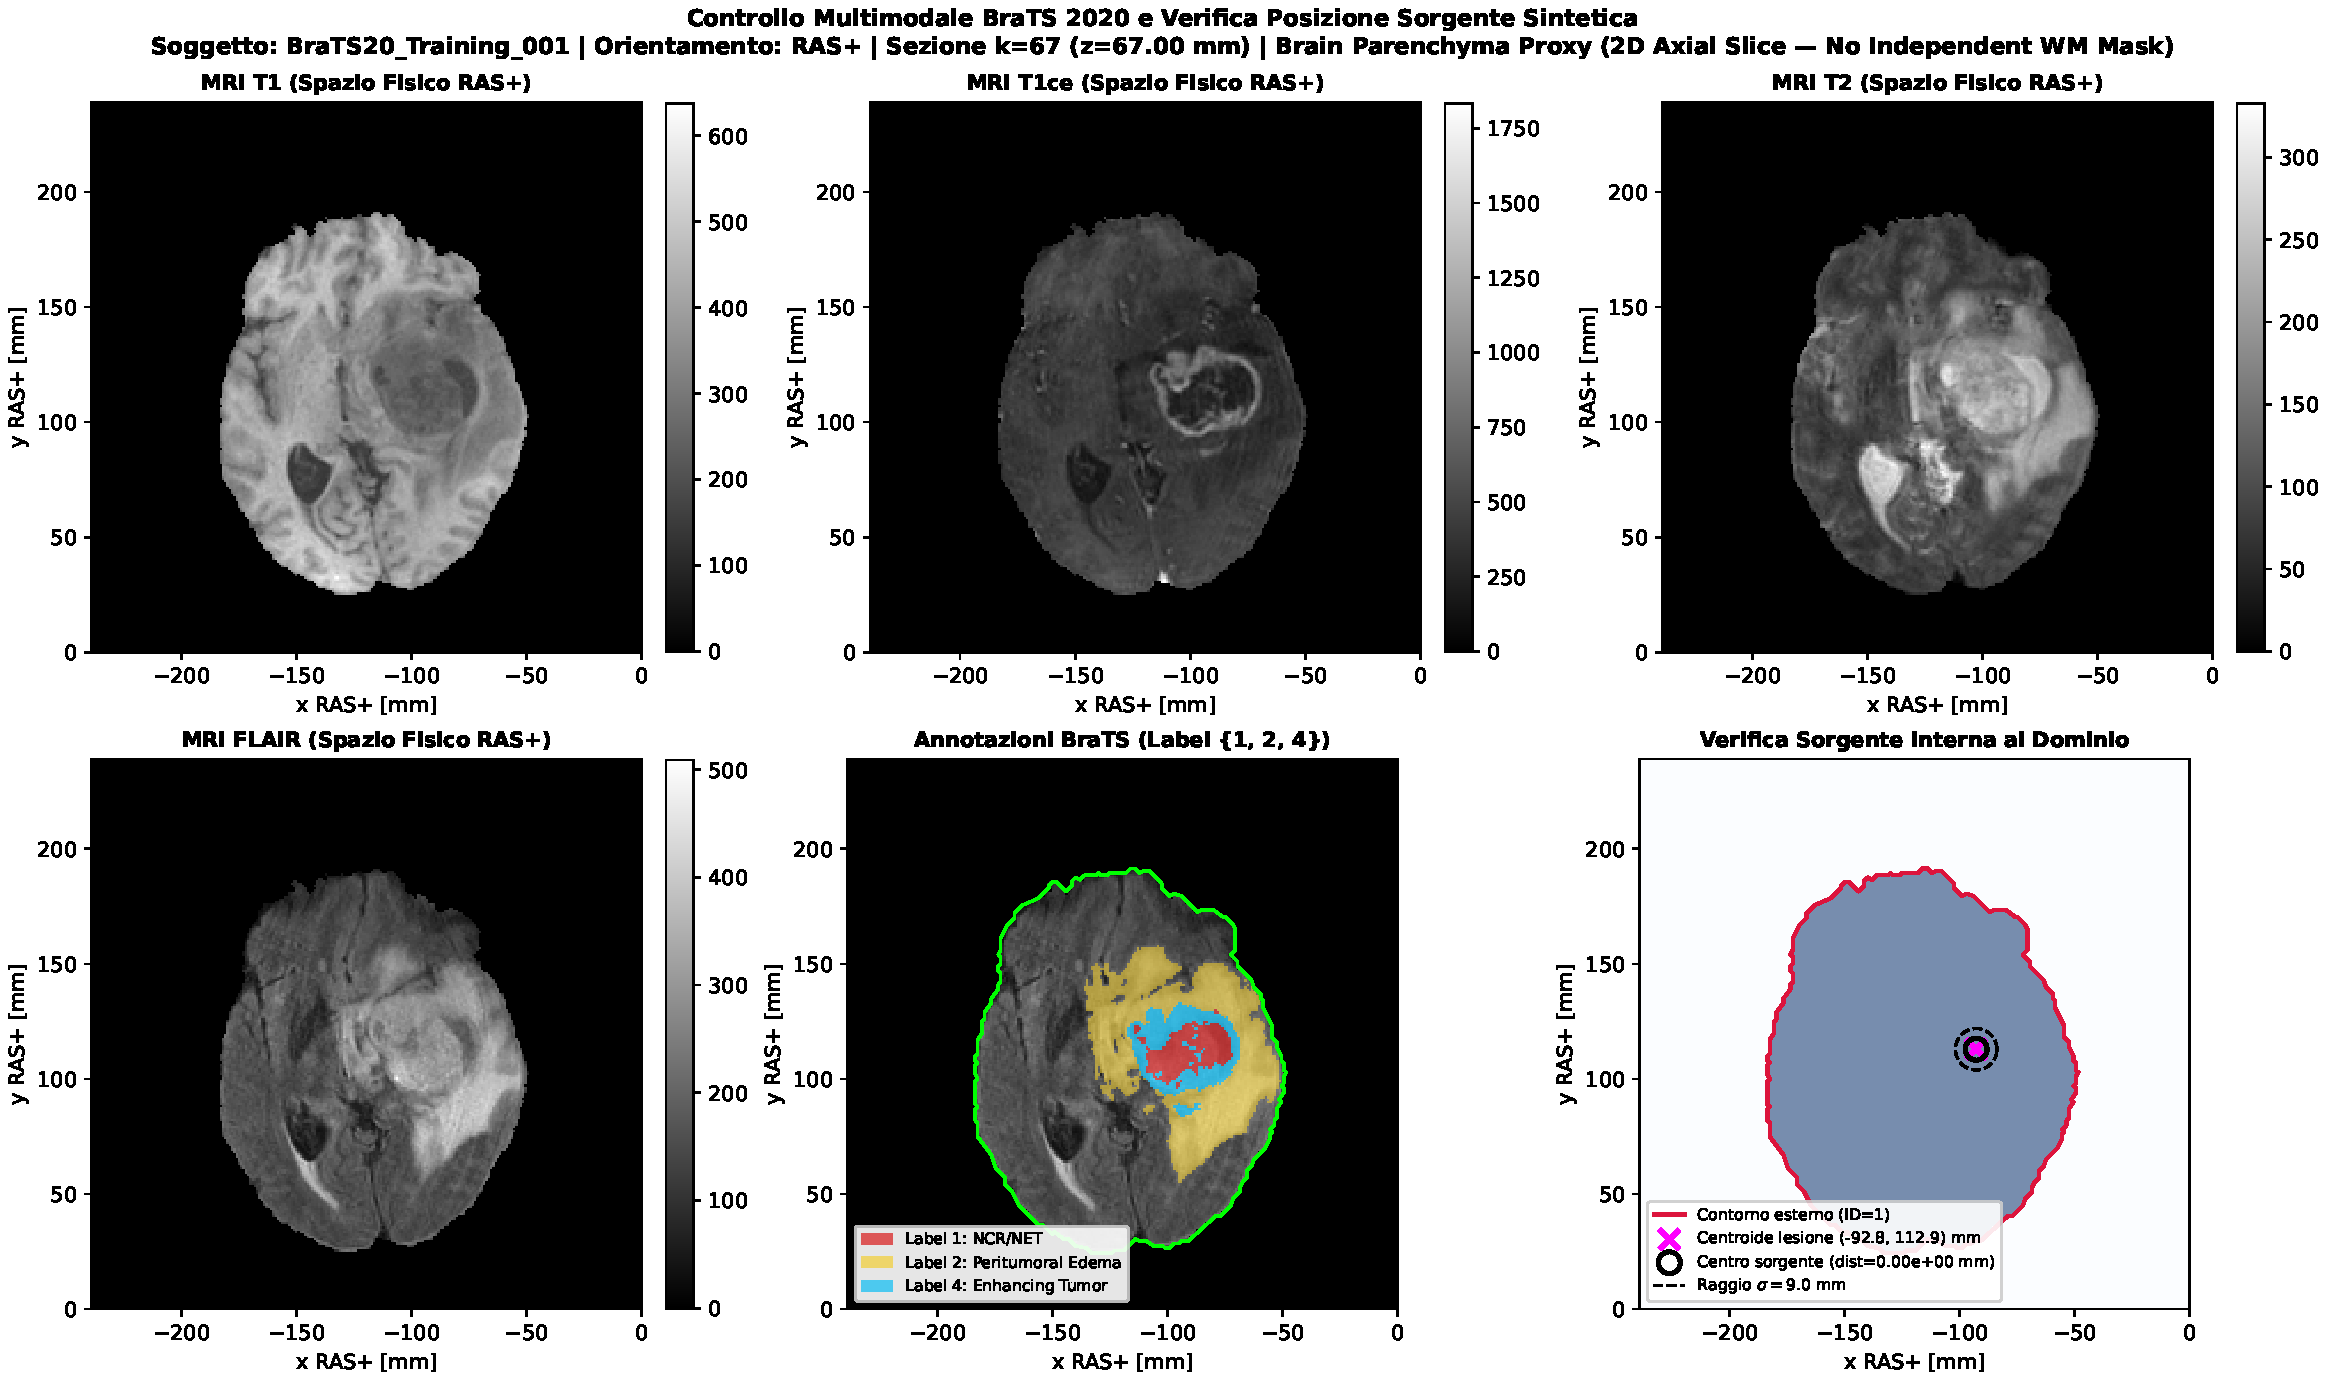
\includegraphics[width=0.94\textwidth]{paper/fig01_multimodal_anatomy_and_annotations.pdf}
\caption{Quattro modalità MRI e annotazioni del caso BraTS selezionato. L'immagine fornisce anatomia statica e localizzazione della lesione; non contiene le traiettorie temporali simulate dal modello.}
\label{fig:anatomy}
\end{figure*}

\begin{figure*}[t]
\centering
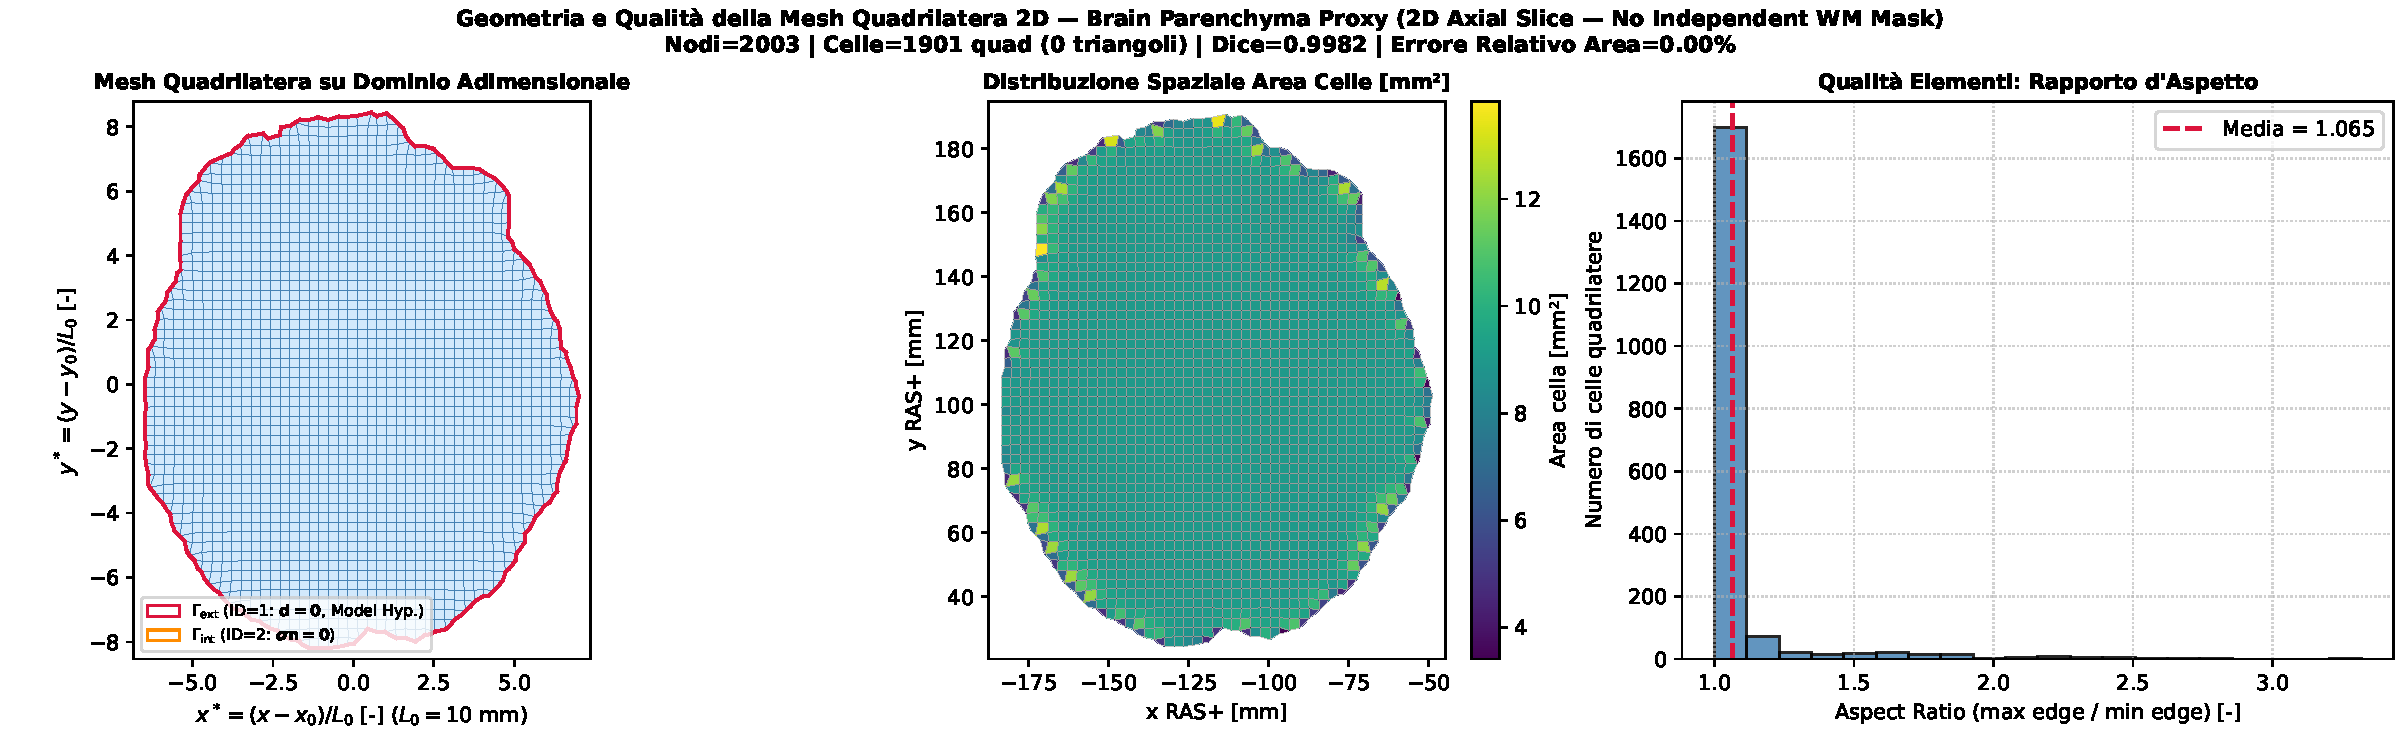
\includegraphics[width=0.94\textwidth]{paper/fig02_anatomical_mask_and_quad_mesh_quality.pdf}
\caption{Dominio proxy e mesh quadrilatera. Le metriche valutano l'approssimazione della maschera scelta, non l'accuratezza istologica o la segmentazione della sostanza bianca.}
\label{fig:mesh}
\end{figure*}

\subsection{Identificabilità e twin experiments sintetici}

L'esperimento di identificabilità usa soltanto osservazioni del tracciante: una griglia spaziale $6\times6$ e cinque istanti adimensionali $t\in\{0.15,0.30,0.50,0.75,1.0\}$, per un totale di $N_{\rm obs}=180$ osservazioni. La discretizzazione inversa di riferimento è $N=16$, $M=80$, $T=1$ e griglia temporale graduata con esponente $r=1.5$, con elementi $Q_2/Q_1/Q_1$. I limiti sono $\alpha,\beta\in[0.15,0.9]$, $D\in[0.01,0.5]$ ed $E\in[0.5,6]$. Il Jacobiano è calcolato con differenze finite centrate nelle coordinate normalizzate, usando passo $10^{-4}$ e pesi identità per le osservazioni adimensionali, in assenza di una covarianza empirica clinica.

Per i twin experiments, il vettore obiettivo è generato sulla discretizzazione $N=32$, $M=160$ e osservato tramite lo stesso insieme di 180 misure; l'inversione di riferimento usa $N=16$, $M=80$. Campo iniziale e callback delle forzanti sono mantenuti identici tra target e inverso, a meno della valutazione sulle rispettive discretizzazioni. Il vettore obiettivo pulito è congelato e identificato dall'hash SHA-256 riportato nell'Appendice~\ref{app:repro}. La campagna senza rumore riutilizza tre run CPSO con budget pianificato di 600 valutazioni del problema diretto. La campagna rumorosa comprende cinque realizzazioni indipendenti per ciascuno dei livelli nominali $\eta\in\{0.05,0.10\}$; per tutte e dieci le run rumorose il seed dell'ottimizzatore è mantenuto fisso, in modo da isolare descrittivamente l'effetto delle realizzazioni del rumore condizionatamente alla medesima configurazione iniziale dello sciame. I seed dei dati rumorosi sono distinti e registrati negli artefatti supplementari.

Nella campagna finale CPSO usa 10 particelle, fino a 60 iterazioni e un budget pianificato di 600 valutazioni FEM per run. Per $\eta=0$ è utilizzata la pesatura deterministica (Mode A) con $\lambda_A=10^{-4}$. Per i casi rumorosi è utilizzata la pesatura con covarianza inversa esatta (Mode B covariance), con $\sigma=\eta\|\mathbf y_{\rm clean}\|_\infty$ e $\lambda_B=7.2$, convertito dalla scala di riferimento $\eta_{\rm ref}=0.05$ secondo $\lambda_B^{\rm eq}(\eta)=N_{\rm obs}\lambda_A/\eta^2$. La scelta mantiene $\lambda_B=7.2$ anche per $\eta=0.10$, per cui non conserva il medesimo rapporto fra dati e penalizzazione nei due livelli: il valore equivalente a $\eta=0.10$ sarebbe $1.8$. Di conseguenza, il confronto tra i due livelli descrive il protocollo effettivamente eseguito e non isola l'effetto del rumore da quello del bilanciamento del funzionale. Il controllo di normalizzazione e di isolamento del target pulito è riportato nell'Appendice~\ref{app:objective}. Il rapporto realizzato $\|\boldsymbol\epsilon\|_2/\|\mathbf y_{\rm clean}\|_2$ è riportato separatamente dal livello nominale, poiché i due valori non coincidono in generale.

Il budget di 600 valutazioni è un limite computazionale, non un criterio di convergenza. Le run finali riportate hanno esaurito il budget e le stime sono pertanto i migliori candidati individuati nelle rispettive storie, non minimi locali o globali certificati. Inoltre, mantenendo fisso il seed CPSO nella campagna rumorosa, la dispersione osservata descrive la sensibilità al rumore per una singola configurazione dell'ottimizzatore, non la variabilità complessiva che deriverebbe anche da seed CPSO indipendenti.

\subsection{Definizione della pesatura obiettivo}

Il confronto dei modi di pesatura valuta tre convenzioni per il residuo $\mathbf r=\mathcal G_h(\boldsymbol\theta)-\mathbf y$: (A) $W_A=I/(\sqrt{N_{\rm obs}}s_{\rm ref})$; (B-mean) $W_{B,\rm mean}=I/(\sqrt{N_{\rm obs}}\sigma)$; (B-cov) $W_{B,\rm cov}=I/\sigma$, con $s_{\rm ref}=\|\mathbf y_{\rm clean}\|_\infty$ e $\sigma=\eta s_{\rm ref}$. Ne segue, a parità di residuo, $J_{\rm data}^{B,\rm mean}/J_{\rm data}^{A}=\eta^{-2}$ e $J_{\rm data}^{B,\rm cov}/J_{\rm data}^{A}=N_{\rm obs}/\eta^2$. I modi non sono intercambiabili mantenendo fisso $\lambda$. L'analisi è un confronto della scala del funzionale su candidati già disponibili, non una nuova ottimizzazione né una regola automatica per calibrare $\lambda$.


\section{Risultati}
\label{sec:results}
\subsection{Verifica MMS e bilanci}

Nella serie spaziale coordinata, gli errori $L^2$ decrescono per tutti i campi. Gli ordini empirici osservati sono circa 2.93--2.97 per lo spostamento, 2.02--2.06 per la pressione e 1.94--1.98 per il tracciante. Gli EOC in $H^1$ sono 1.98--1.99 per lo spostamento, 1.00--1.01 per la pressione e 1.40--1.71 per il tracciante. Questi ultimi valori indicano che il regime asintotico per la seminorma $H^1$ del tracciante non è stato dimostrato.

\begin{table*}[t]
\centering
\caption{Errori spaziali $L^2$ ed ordini di convergenza osservati (EOC) nella serie MMS coordinata. Il parametro $h=1/N$ è la larghezza della cella quadrata, non il diametro diagonale dell'elemento.}
\label{tab:spatial}
\small
\begin{tabular}{ccccccc}
\toprule
$h$ & $\|e_d\|_{L^2}$ & EOC & $\|e_p\|_{L^2}$ & EOC & $\|e_c\|_{L^2}$ & EOC\\
\midrule
0.2500 & $2.687\times10^{-3}$ & -- & $5.453\times10^{-3}$ & -- & $2.456\times10^{-2}$ & --\\
0.1250 & $3.529\times10^{-4}$ & 2.93 & $1.305\times10^{-3}$ & 2.06 & $6.396\times10^{-3}$ & 1.94\\
0.0625 & $4.493\times10^{-5}$ & 2.97 & $3.229\times10^{-4}$ & 2.02 & $1.616\times10^{-3}$ & 1.98\\
\bottomrule
\end{tabular}
\end{table*}

Nel raffinamento temporale con spazio $Q_2/Q_2/Q_2$, per $\Delta t_{\max}=0.05,0.025,0.0125,0.00625$, gli EOC dell'ultimo intervallo sono rispettivamente 1.06, 0.99 e 0.99 per $d,p,c$. Una diagnostica ulteriore, eseguita a mesh fissa e raddoppiando il numero di passi da 4800 a 9600, ha prodotto variazioni relative delle norme finali pari a 0.02\% per $d$, 0.75\% per $p$ e 3.24\% per $c$. Il contributo temporale per il tracciante non è quindi trascurabile in ogni regime; gli EOC della serie coordinata sono risultati osservati, non una prova isolata degli ordini spaziali teorici. Le tabelle complete sono riportate nell'Appendice A.

\begin{figure*}[t]
\centering
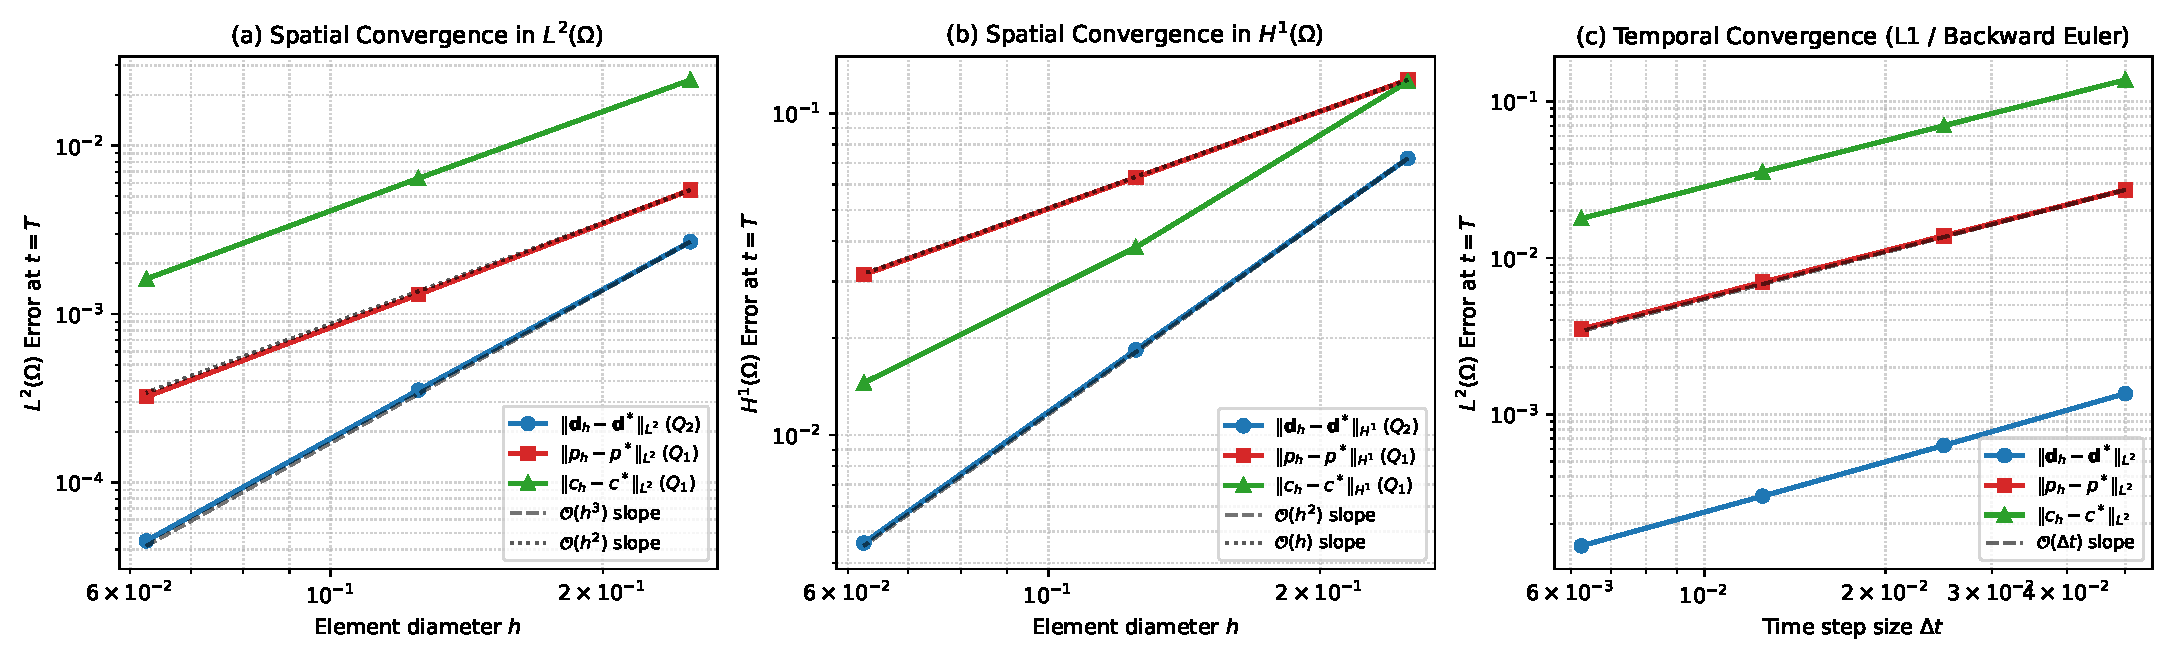
\includegraphics[width=0.94\textwidth]{paper/fig03_mms_convergence_complete.pdf}
\caption{Verifica MMS: errori spaziali $L^2$ e $H^1$ e raffinamento temporale $L^2$ per i tre campi. I tassi rappresentano il protocollo numerico eseguito; l'isolamento dell'errore spaziale richiede la cautela descritta nel testo.}
\label{fig:mms}
\end{figure*}

Sul quadrato, il residuo di compatibilità iniziale è $5.45\times10^{-16}$, l'errore massimo dell'identità algebrica passo-passo è $4.78\times10^{-17}$ e il drift relativo della massa del tracciante è $3.92\times10^{-15}$. Riducendo $\Delta t$ da 0.04 a 0.005, il residuo energetico cumulativo assoluto scende da $2.074\times10^{-3}$ a $2.903\times10^{-4}$. L'identità algebrica passo-passo è un controllo distinto dal residuo energetico cumulativo e non dimostra, da sola, una disuguaglianza energetica discreta generale.

\subsection{Geometria e campi della simulazione anatomica}

La maschera selezionata ha area $17069\,\mathrm{mm}^2$ e la mesh di riferimento area $17068.29\,\mathrm{mm}^2$, con errore relativo $4.17\times10^{-5}$, Dice rasterizzato 0.9982 e IoU 0.9963. Tutte le 1901 celle sono quadrilatere; non sono state rilevate celle invertite o degeneri. Questo conferma la fedeltà della mesh alla maschera definita, non la correttezza istologica della maschera. La forma anatomica è classificata come proxy del parenchima e non come sostanza bianca segmentata.

\begin{figure*}[t]
\centering
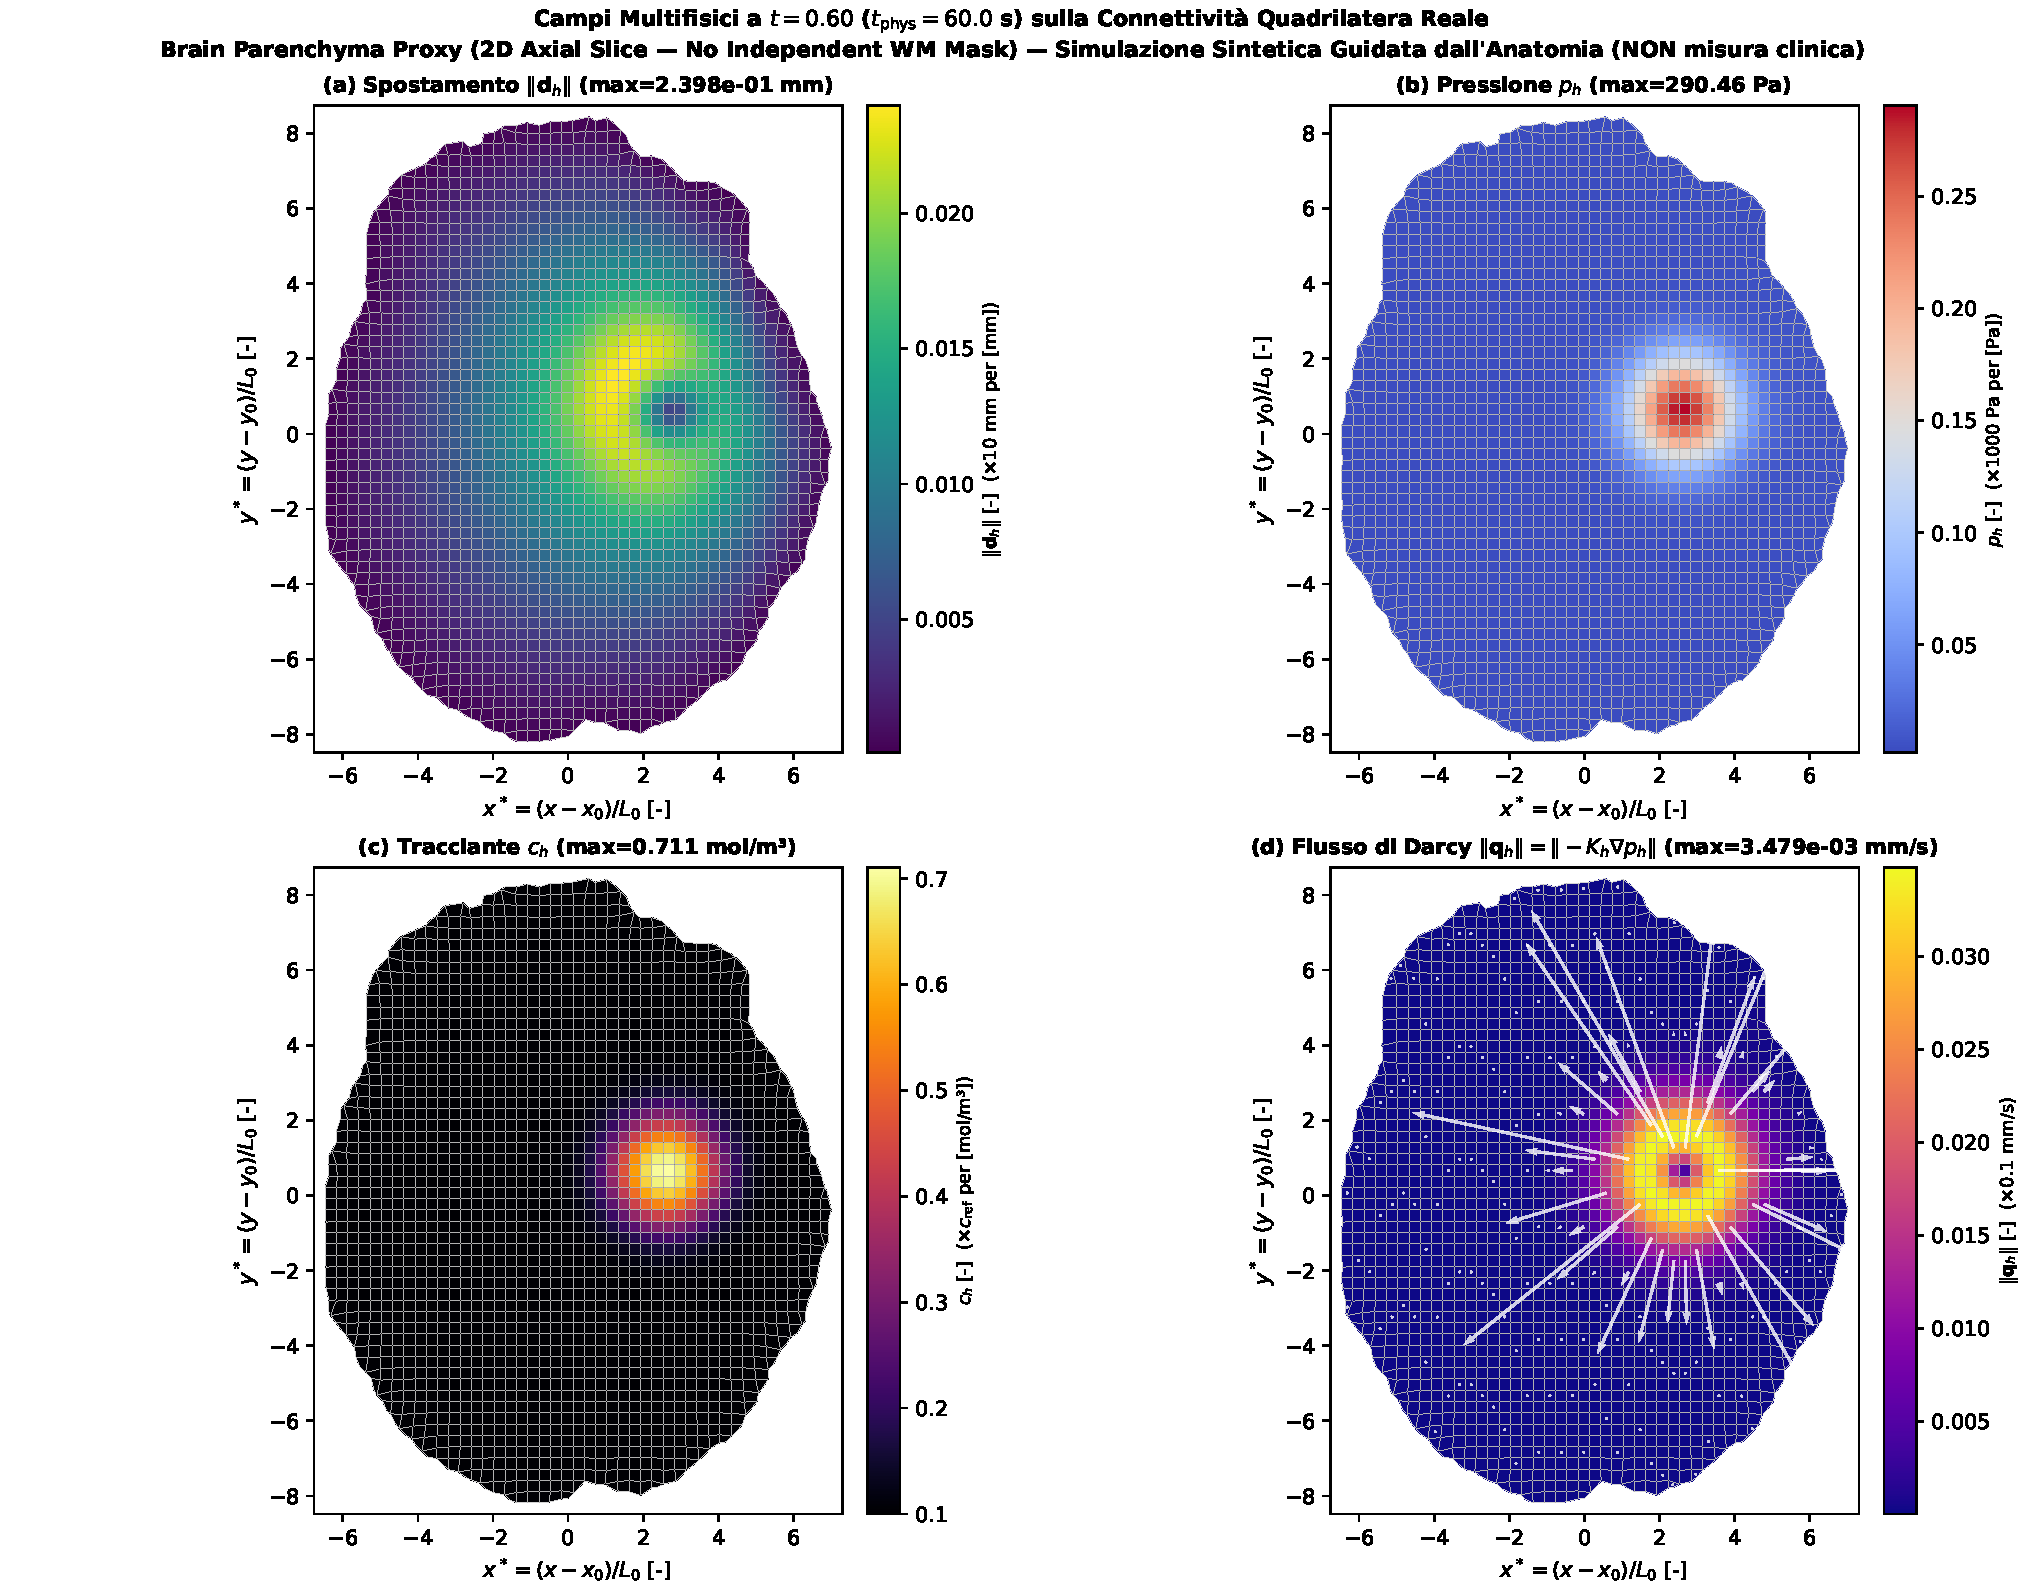
\includegraphics[width=0.94\textwidth]{paper/fig04_multiphysics_fields_on_quad_mesh.pdf}
\caption{Campi finali calcolati sulla connettività quadrilatera derivata dalla sezione BraTS. La sorgente è ancorata al centroide della lesione; ampiezze e andamenti temporali sono sintetici e non corrispondono a misure cliniche.}
\label{fig:fields}
\end{figure*}

La traiettoria anatomica ha norme finali adimensionali $\|d_h(T)\|_{L^2}=0.12105$, $\|p_h(T)\|_{L^2}=0.53803$ e $\|c_h(T)\|_{L^2}=1.97108$. La velocità di Darcy massima è 0.03678 adimensionale, equivalente a $3.68\times10^{-3}$ mm/s con le scale dichiarate. Sono statistiche della traiettoria forzata dal protocollo sintetico, non stime di variabili cliniche.

Il test di sensibilità alla mesh confronta dimensioni di lato obiettivo 4, 3 e 2 mm. Rispetto alla mesh da 2 mm, le differenze relative per la norma finale del tracciante sono 0.431\% (4 mm) e 0.186\% (3 mm); per la norma dello spostamento 0.562\% e 0.253\%; per l'energia totale finale 2.111\% e 0.895\%. Poiché non è disponibile una soluzione esatta sul dominio anatomico, tali differenze sono sensibilità alla discretizzazione, non ordini di convergenza. L'evoluzione temporale e le curve di sensibilità frazionaria sono raccolte nell'Appendice B.

\subsection{Conservazione e diagnostica energetica sulla mesh anatomica}

Sulla mesh da 3 mm, la massa adimensionale del tracciante passa da 21.08953037267824 a 21.089530372678244, con drift relativo massimo $6.74\times10^{-16}$. L'errore massimo dell'identità algebrica passo-passo è $7.65\times10^{-17}$. Al tempo finale, l'energia totale è 0.08551, la dissipazione viscoelastica cumulativa 0.00451, quella idraulica 0.01571 e il lavoro esterno cumulativo 0.10761; il residuo energetico cumulativo registrato è $-1.88\times10^{-3}$. Poiché i carichi sono attivi, l'energia totale non è attesa decrescere monotonicamente. Questi dati documentano il bilancio numerico del caso eseguito, non una prova generale della stabilità energetica dello schema.

\begin{figure*}[t]
\centering
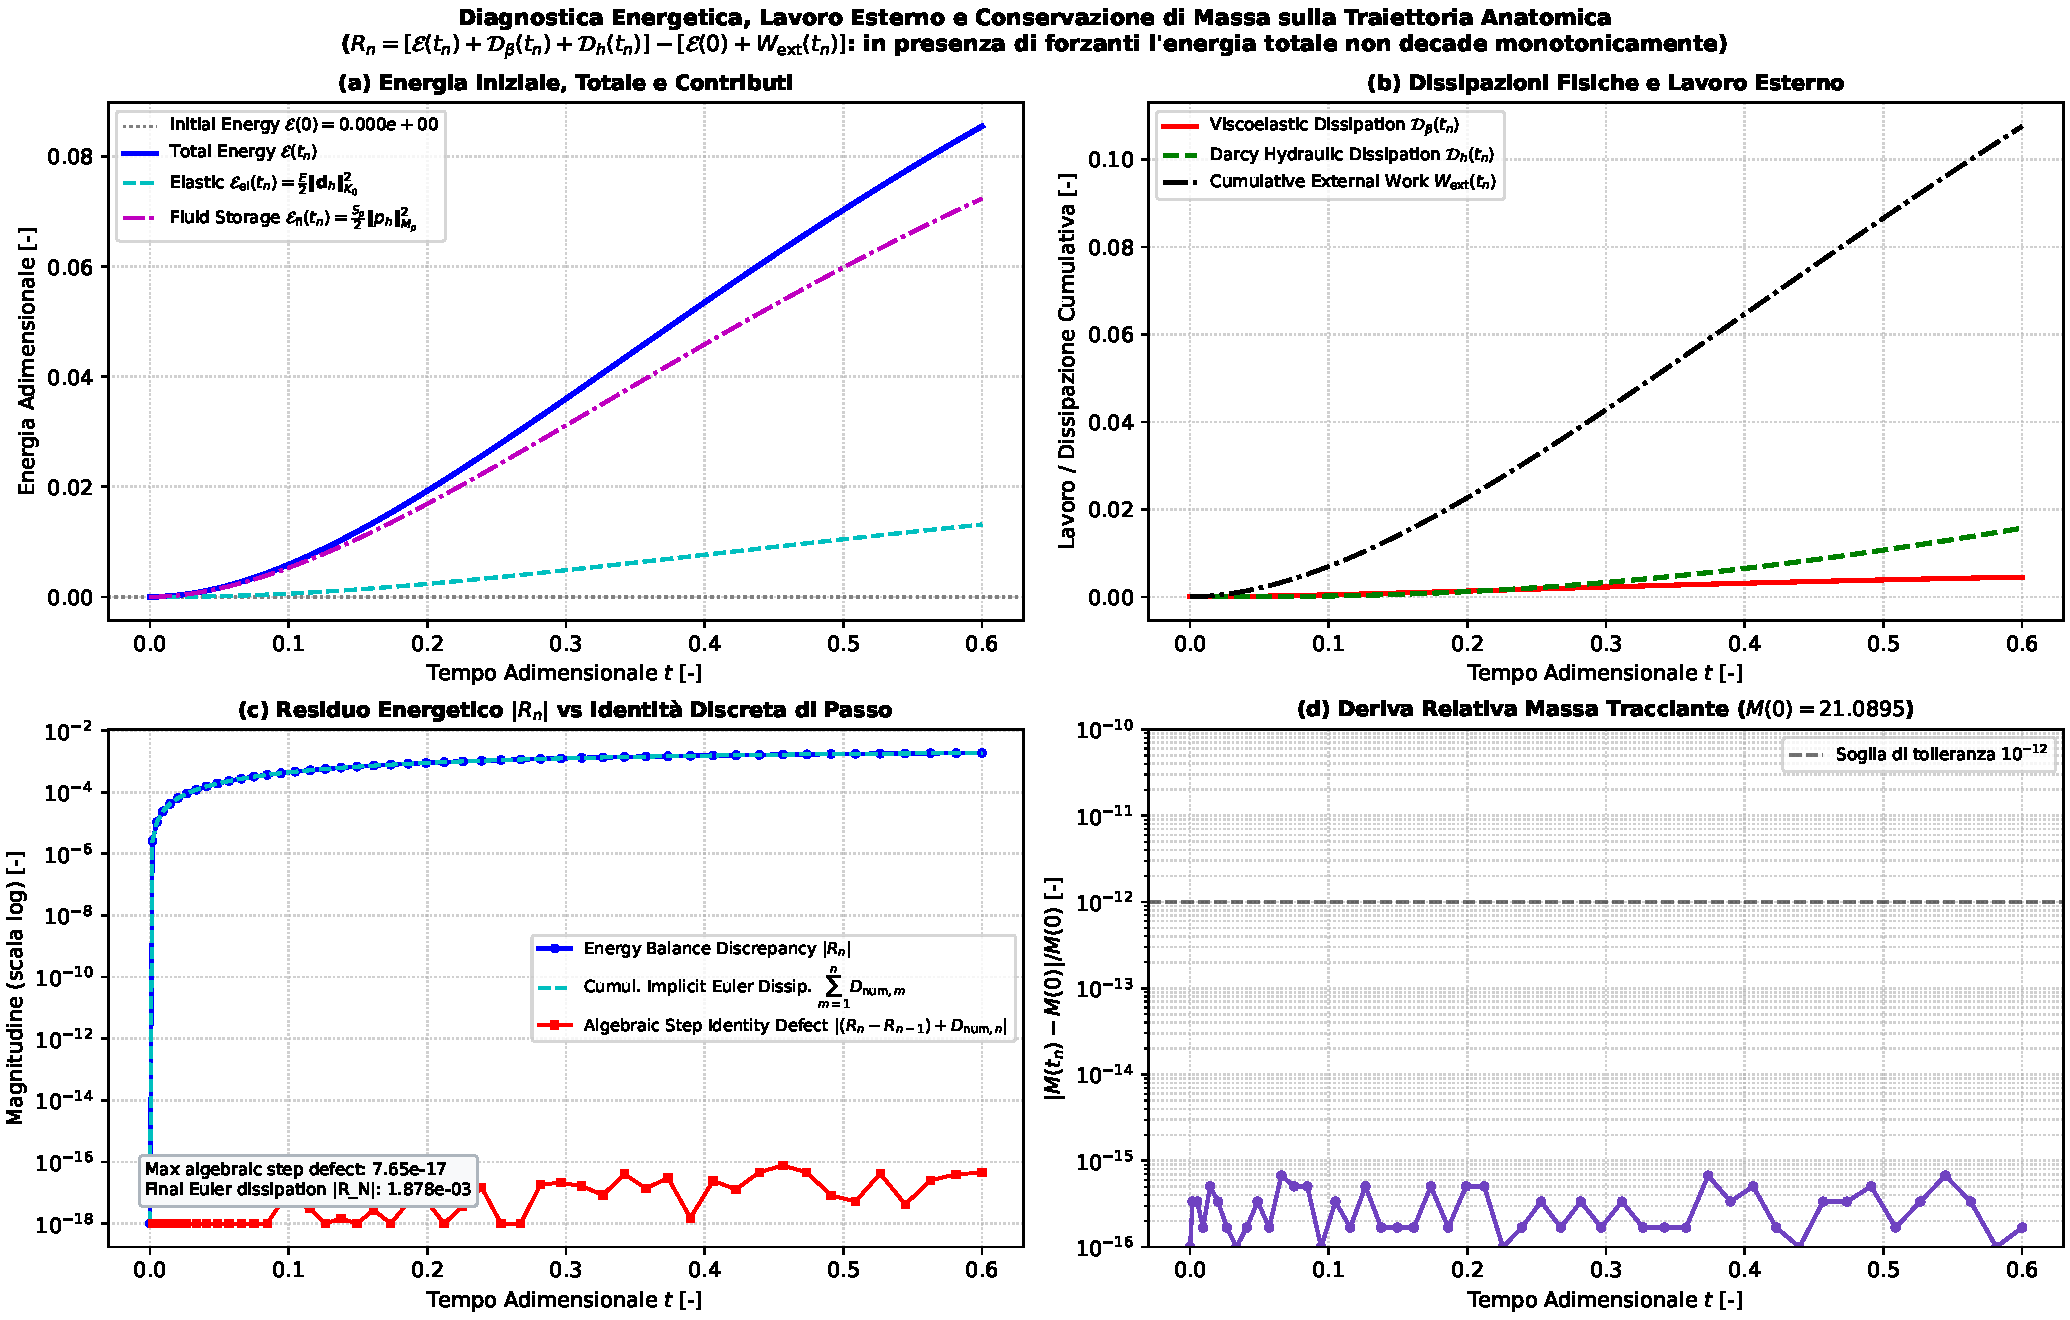
\includegraphics[width=0.94\textwidth]{paper/fig05_energy_and_mass_diagnostics.pdf}
\caption{Diagnostiche energetiche e di massa sulla traiettoria anatomica forzata. L'identità discreta passo-passo e il residuo globale sono mostrati come grandezze distinte.}
\label{fig:energy}
\end{figure*}

\subsection{Identificabilità locale: flusso nullo e flusso attivo}

Con sole osservazioni del tracciante, nel protocollo a flusso nullo tutte le nove traiettorie di perturbazione confermano $\mathbf q=0$, $p=0$ e $d=0$ entro la tolleranza configurata. Il Jacobiano discreto ha rango numerico 2: le colonne associate ad $\beta$ ed $E$ sono esattamente nulle e i valori singolari sono $(1.5833,0.3222,0,0)$. Questo è il riscontro numerico della Proposizione~\ref{prop:zeroq} nel protocollo testato.

Con il protocollo di carico attivo, il massimo della velocità di Darcy alla configurazione di riferimento è 0.05910 adimensionale e il Jacobiano ha rango numerico 4. I valori singolari sono $(1.2325,0.3784,0.3047,0.05229)$ e il numero di condizionamento è 23.57 secondo la convenzione del report. Il modo destro meno informativo è dominato da $\beta$ (componente circa $-0.9965$). La stabilità al passo di differenza finita è buona: variando il passo tra $10^{-3}$ e $10^{-5}$, la differenza relativa di Frobenius rispetto al Jacobiano di riferimento è al massimo $1.51\times10^{-6}$. Il rango pieno è evidenza di identificabilità locale regolare per quella mappa discreta e quel punto, non identificabilità globale né garanzia statistica di precisione.

\begin{figure*}[t]
\centering
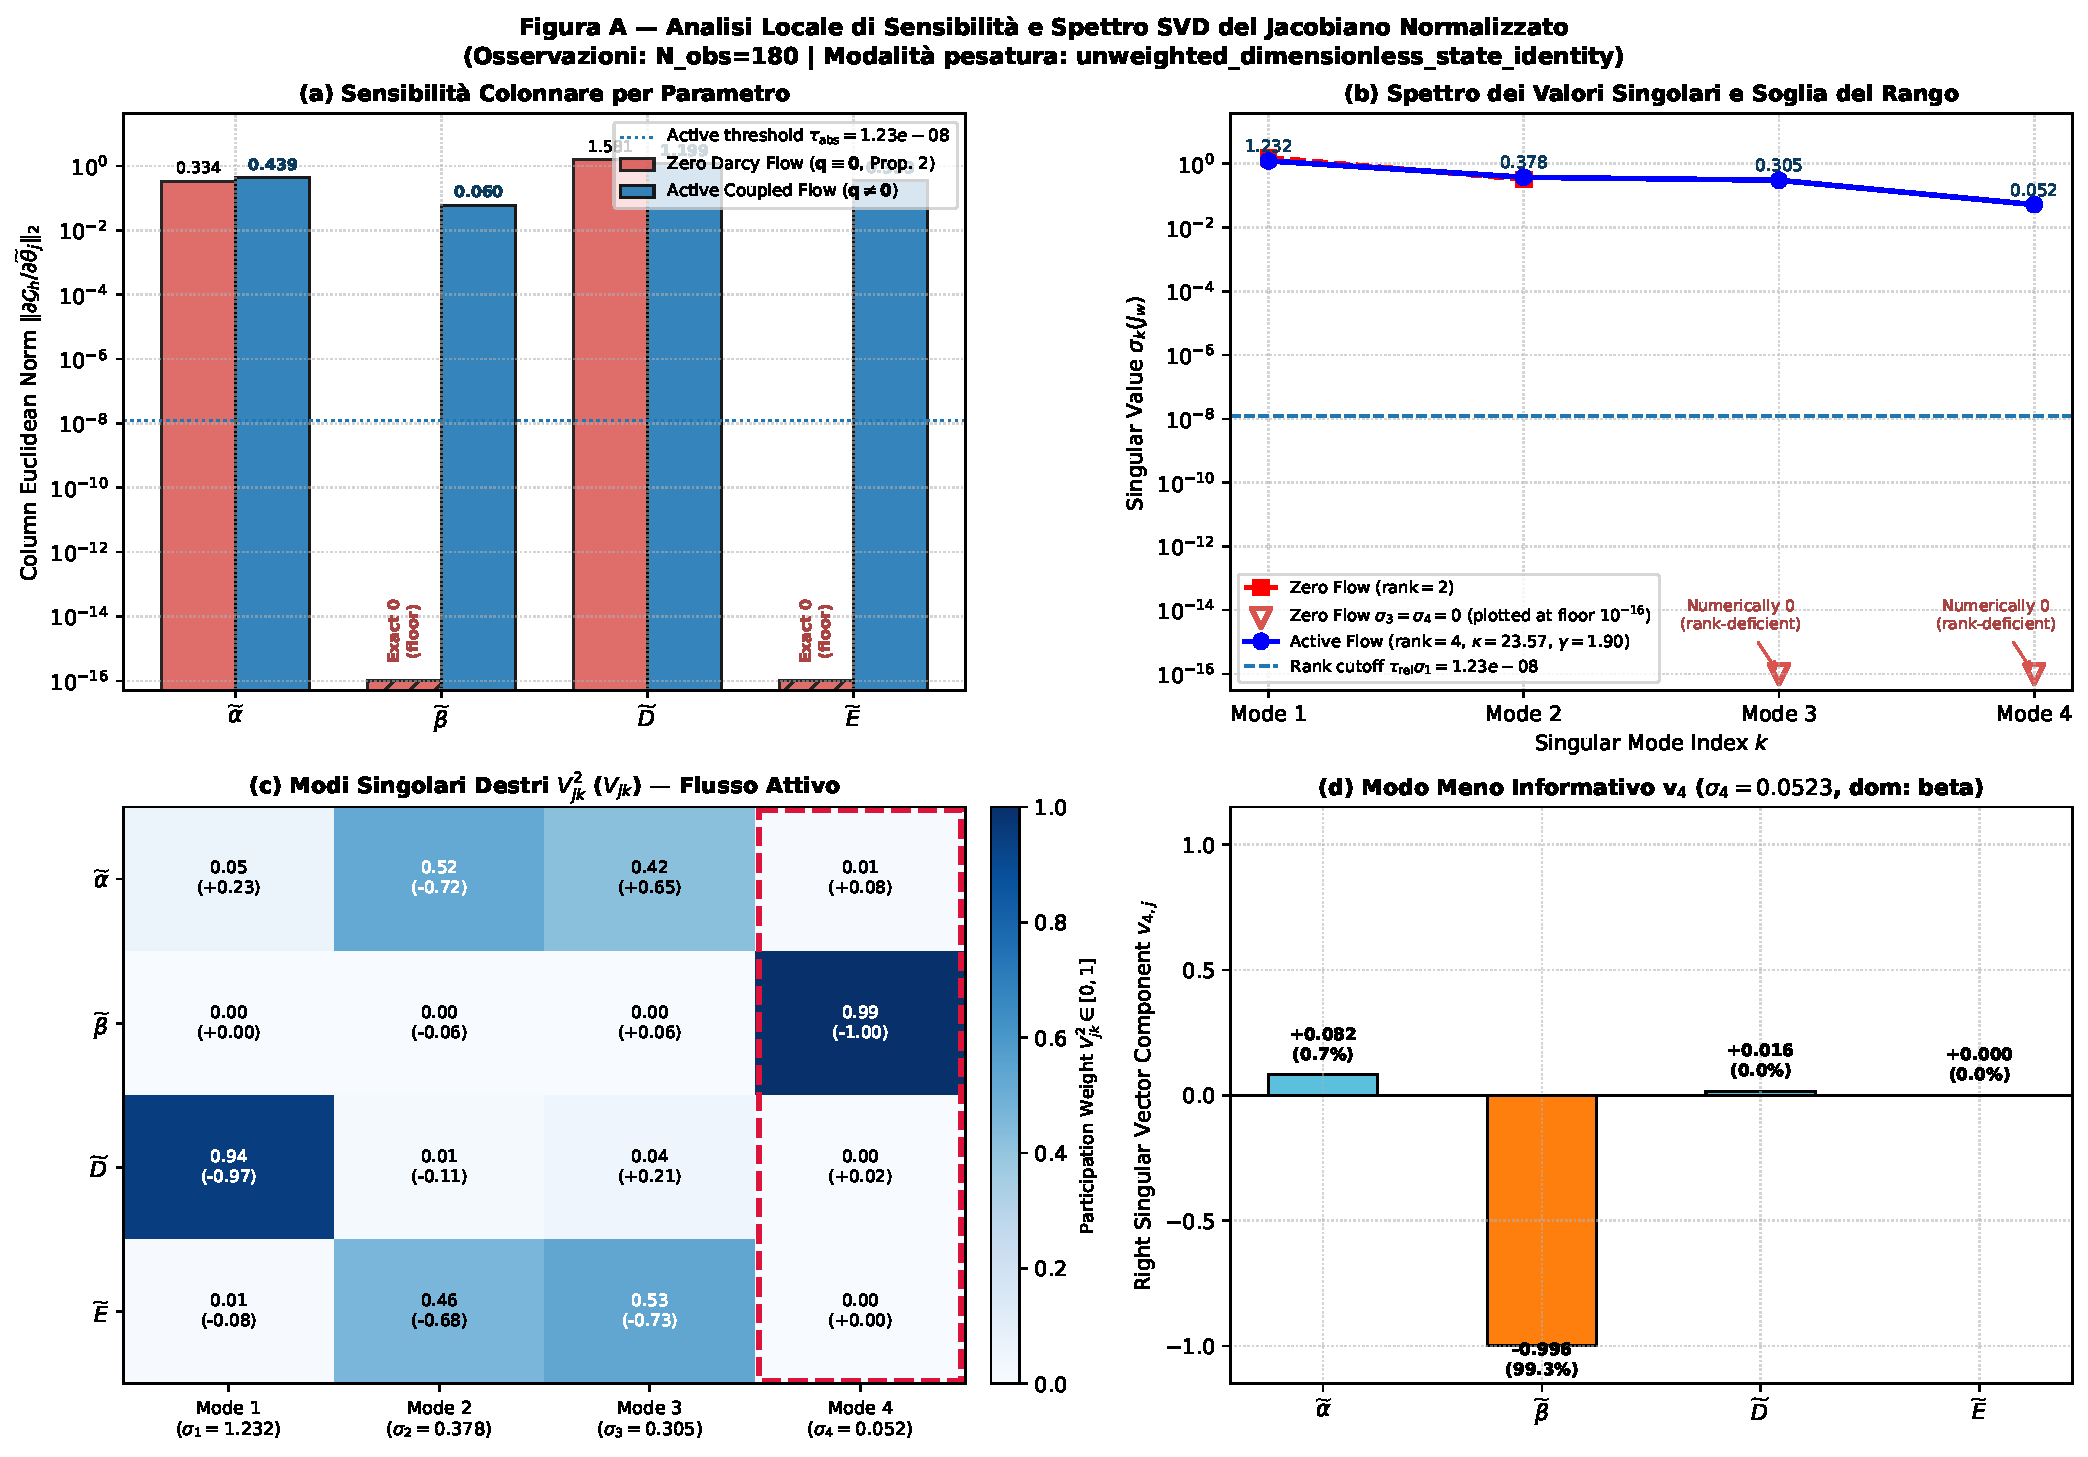
\includegraphics[width=0.94\textwidth]{paper/fig06_sensitivity_and_svd.pdf}
\caption{Diagnostica del Jacobiano osservativo normalizzato: degenerazione esatta nel protocollo a flusso nullo e rango pieno nel protocollo con flusso attivo. L'analisi è locale e non pesata da una covarianza clinica empirica.}
\label{fig:identifiability}
\end{figure*}

Le curve one-at-a-time, che variano un parametro alla volta mantenendo gli altri a $\tht^\dagger$, non includono il compensarsi simultaneo dei parametri. I profili ottimizzati, invece, riottimizzano gli altri parametri ma sono scansioni numeriche del funzionale sintetico e non profili di verosimiglianza statistici. I dettagli sono nell'Appendice C.

\subsection{Profili ottimizzati rispetto a \texorpdfstring{$\beta$}{beta} e sensibilità alla discretizzazione}

Per distinguere la sensibilità del termine dati dall'effetto della penalizzazione, sono stati calcolati due profili numerici bidirezionali su 15 valori di $\beta\in[0.15,0.90]$: $\Phi_{\rm data}(\beta)=\min_{\alpha,D,E}J_{\rm data}$ e $\Phi_{\lambda}(\beta)=\min_{\alpha,D,E}J_{\rm total}$. La scansione è stata eseguita sulla discretizzazione inversa $N=16$, $M=80$, mantenendo fisso il target sintetico e senza utilizzare $\boldsymbol\theta^\dagger$ nell'ottimizzazione. Il minimo campionato di $\Phi_{\rm data}$ si trova in $\beta=0.4500$; quello di $\Phi_{\lambda}$ in $\beta=0.479143$. Le regioni campionate entro il 25\% del minimo sono rispettivamente $[0.425,0.450]$ e $[0.425,0.525]$. La maggiore ampiezza del secondo intervallo è coerente con l'interazione tra il termine dati e la regolarizzazione: il prior normalizzato $\widetilde\beta_0=0.5$ corrisponde a $\beta=0.525$ nei limiti fisici adottati e contribuisce quindi a spostare il minimo del funzionale totale.

\begin{table*}[t]
\centering
\caption{Sintesi dei profili ottimizzati campionati rispetto a $\beta$ sulla discretizzazione inversa $N=16$, $M=80$. Gli intervalli sono insiemi di punti della griglia entro la soglia indicata; non sono intervalli di confidenza statistici.}
\label{tab:beta-profiles}
\small
\begin{tabular}{lcccc}
\toprule
Profilo & $\beta$ al minimo campionato & Valore minimo & Regione entro $+10\%$ & Regione entro $+25\%$\\
\midrule
$\Phi_{\rm data}$ & $0.450000$ & $3.4581\times10^{-7}$ & $[0.450,0.450]$ & $[0.425,0.450]$\\
$\Phi_{\lambda}$ & $0.479143$ & $4.4657\times10^{-6}$ & $[0.450,0.500]$ & $[0.425,0.525]$\\
\bottomrule
\end{tabular}
\end{table*}

Le scansioni forward e backward individuano lo stesso valore campionato di $\beta$ per entrambi i profili. Tuttavia, alcuni punti della griglia hanno esaurito il budget interno per direzione: 13/15 punti backward convergono per il profilo dati e 14/15 per ciascuna direzione del profilo regolarizzato. La concordanza dei minimi campionati è dunque una verifica di consistenza numerica, non una dimostrazione di ottimalità globale. Inoltre, $\Phi_{\rm data}$ e $\Phi_{\lambda}$ sono profili del funzionale deterministico usato nell'esperimento, non profili di verosimiglianza statistici.

La sensibilità alla discretizzazione inversa è stata verificata riutilizzando lo stesso target sintetico $N=32$, $M=160$ e confrontando $N=16$, $M=80$ con $N=24$, $M=120$. Sulla griglia locale comune di $\beta$, il minimo campionato del profilo dati si sposta da $0.4500$ a $0.4375$; le stime dei parametri di disturbo $(\alpha,D,E)$ al minimo restano vicine. Il costo al parametro vero diminuisce di un fattore 2.22 e il minimo del profilo campionato di un fattore 3.53 passando alla discretizzazione più fine. Questa variazione documenta la sensibilità del funzionale all'errore di discretizzazione; non è, da sola, una prova di convergenza del problema inverso.

\begin{table*}[t]
\centering
\caption{Sensibilità del profilo dati alla discretizzazione inversa. I minimi sono minimi campionati sulla griglia locale comune, non minimi globali certificati.}
\label{tab:beta-mesh-sensitivity}
\small
\begin{tabular}{lccccc}
\toprule
Griglia inversa & $J_{\rm data}(\boldsymbol\theta^\dagger)$ & Residuo rel. & $\beta_{\min}$ & $\min\Phi_{\rm data}$ & $(\widehat\alpha,\widehat D,\widehat E)$\\
\midrule
$(16,80)$ & $6.2194\times10^{-7}$ & $1.9373\times10^{-3}$ & $0.4500$ & $3.4581\times10^{-7}$ & $(0.7003,0.07932,2.4878)$\\
$(24,120)$ & $2.8055\times10^{-7}$ & $1.3012\times10^{-3}$ & $0.4375$ & $9.8005\times10^{-8}$ & $(0.7007,0.07937,2.5097)$\\
\bottomrule
\end{tabular}
\end{table*}

\subsection{Twin experiments senza rumore: budget esteso}

La campagna senza rumore comprende tre run CPSO con budget pianificato di 600 valutazioni FEM, selezionate dagli artefatti preesistenti senza rieseguire l'ottimizzazione. La soluzione con il valore più basso osservato di $J_{\rm total}$ è la run con seed 20261018, che restituisce $\widehat{\boldsymbol\theta}=(0.6956,0.4791,0.07892,2.4805)$ e residuo relativo rispetto al target pulito pari allo $0.192\%$. Le altre due run mostrano una stima di $\beta$ più distante dal valore vero, pur recuperando $\alpha$, $D$ ed $E$ con errori generalmente inferiori a pochi punti percentuali.

\begin{table*}[t]
\centering
\caption{Tre run CPSO senza rumore con budget pianificato di 600 valutazioni FEM. La run selezionata è quella con il valore minimo osservato di $J_{\rm total}$; nessuna run è certificata convergente.}
\label{tab:baseline-600}
\small
\begin{tabular}{rcrrrrrc}
\toprule
Seed CPSO & Selezionata & $\widehat\alpha$ & $\widehat\beta$ & $\widehat D$ & $\widehat E$ & $J_{\rm total}$ & Residuo pulito [\%]\\
\midrule
20261017 & No & 0.7033 & 0.3880 & 0.07952 & 2.4788 & $6.3224\times10^{-6}$ & 0.2118\\
20261018 & Sì & 0.6956 & 0.4791 & 0.07892 & 2.4805 & $4.4668\times10^{-6}$ & 0.1918\\
20261019 & No & 0.6838 & 0.6033 & 0.07755 & 2.4870 & $8.9289\times10^{-6}$ & 0.5524\\
\bottomrule
\end{tabular}
\end{table*}

Tutte le tre run hanno terminato per esaurimento del budget, non per un criterio di convergenza. La dispersione di $\widehat\beta$ (da 0.3880 a 0.6033) è considerevole rispetto a quella degli altri parametri e concorda con la struttura dei profili: nell'intervallo centrale, differenti combinazioni parametriche possono produrre valori del termine dati dello stesso ordine. Il minimo osservato di $J_{\rm total}$ identifica il miglior candidato trovato nella campagna, non dimostra un minimo globale e non quantifica da solo l'incertezza statistica.

\subsection{Robustezza al rumore: dieci realizzazioni sintetiche}

La campagna rumorosa comprende cinque realizzazioni indipendenti a ciascun livello nominale $\eta=0.05$ e $\eta=0.10$, con seed CPSO mantenuto fisso e seed del rumore distinti. Il livello nominale è definito attraverso la scala $L^\infty$ del target, mentre la tabella riporta separatamente il rapporto realizzato $\|\boldsymbol\epsilon\|_2/\|\mathbf y_{\rm clean}\|_2$: quest'ultimo varia dall'8.41\% al 9.49\% per $\eta=0.05$ e dal 15.96\% al 17.95\% per $\eta=0.10$.

\begin{table*}[t]
\centering
\caption{Recupero parametrico nella campagna rumorosa finale. Sono riportate mediana, minimo e massimo empirici su cinque realizzazioni per livello. Con $n=5$, questi riepiloghi descrivono il campione e non costituiscono intervalli di confidenza.}
\label{tab:noisy-median-summary}
\small
\begin{tabular}{cccrcc}
\toprule
$\eta$ nominale & $n$ & Parametro & Valore vero & Stima mediana [min, max] & Errore relativo mediano [min, max] [\%]\\
\midrule
0.05 & 5 & $\alpha$ & 0.70 & $0.7027\ [0.6447,0.7301]$ & $3.94\ [0.38,7.90]$\\
0.05 & 5 & $\beta$ & 0.45 & $0.4020\ [0.3562,0.5192]$ & $15.37\ [8.47,20.85]$\\
0.05 & 5 & $D$ & 0.08 & $0.08064\ [0.07603,0.08758]$ & $4.71\ [0.79,9.47]$\\
0.05 & 5 & $E$ & 2.50 & $2.6127\ [2.2431,3.1846]$ & $10.28\ [0.99,27.38]$\\
\midrule
0.10 & 5 & $\alpha$ & 0.70 & $0.6847\ [0.6272,0.7478]$ & $4.48\ [2.16,10.40]$\\
0.10 & 5 & $\beta$ & 0.45 & $0.4234\ [0.3476,0.4754]$ & $5.91\ [1.23,22.76]$\\
0.10 & 5 & $D$ & 0.08 & $0.07587\ [0.06897,0.08816]$ & $5.95\ [3.15,13.79]$\\
0.10 & 5 & $E$ & 2.50 & $2.2282\ [1.6559,2.7267]$ & $10.87\ [1.53,33.76]$\\
\bottomrule
\end{tabular}
\end{table*}

La Figura~\ref{fig:cpso-final-convergence} mostra la cronologia del miglior costo osservato nelle tre run senza rumore e nelle dieci run rumorose. Gli errori non seguono un andamento monotono rispetto a $\eta$: ad esempio, l'errore mediano di $\beta$ è maggiore nel campione a $\eta=0.05$ rispetto a quello a $\eta=0.10$. Questo comportamento, insieme all'ampiezza degli intervalli min--max di $E$ e $\beta$, impedisce di sostenere che il recupero peggiori in modo regolare con il rumore o che il metodo sia robusto in senso generale. Inoltre, il seed dell'ottimizzatore è fisso nella campagna rumorosa: per separare la variabilità dovuta al rumore da quella intrinseca al CPSO occorrerebbe un disegno fattoriale con più seed dell'ottimizzatore per ciascuna realizzazione.

Tutte le dieci run rumorose hanno esaurito il budget pianificato di 600 valutazioni FEM e nessuna ha ottenuto un certificato di convergenza. La funzione obiettivo usa la covarianza inversa esatta e $\lambda_B=7.2$ calibrato alla scala di riferimento $\eta_{\rm ref}=0.05$. Il bilanciamento fra dati e penalizzazione dipende però dal livello $\eta$: con le normalizzazioni dichiarate nell'Equazione~\ref{eq:weight-ratios}, il valore equivalente è $\lambda_B^{\rm eq}(\eta)=N_{\rm obs}\lambda_A/\eta^2$, quindi $7.2$ per $\eta=0.05$ e $1.8$ per $\eta=0.10$. Il protocollo eseguito mantiene invece $\lambda_B=7.2$ in entrambi i gruppi; rispetto al bilanciamento equivalente, la penalizzazione ha quindi peso relativo quattro volte maggiore nel gruppo $\eta=0.10$. I risultati descrivono pertanto la campagna effettivamente eseguita, nella quale cambiano sia il rumore sia il rapporto fra termine dati e regolarizzazione, e non isolano l'effetto del rumore. I valori grezzi di $J_{\rm data}$ ai due livelli non vanno confrontati come se fossero sulla stessa scala. I dettagli per run e l'audit del funzionale sono riportati nelle Appendici~\ref{app:noise} e~\ref{app:objective}.

\begin{figure*}[!t]
\centering
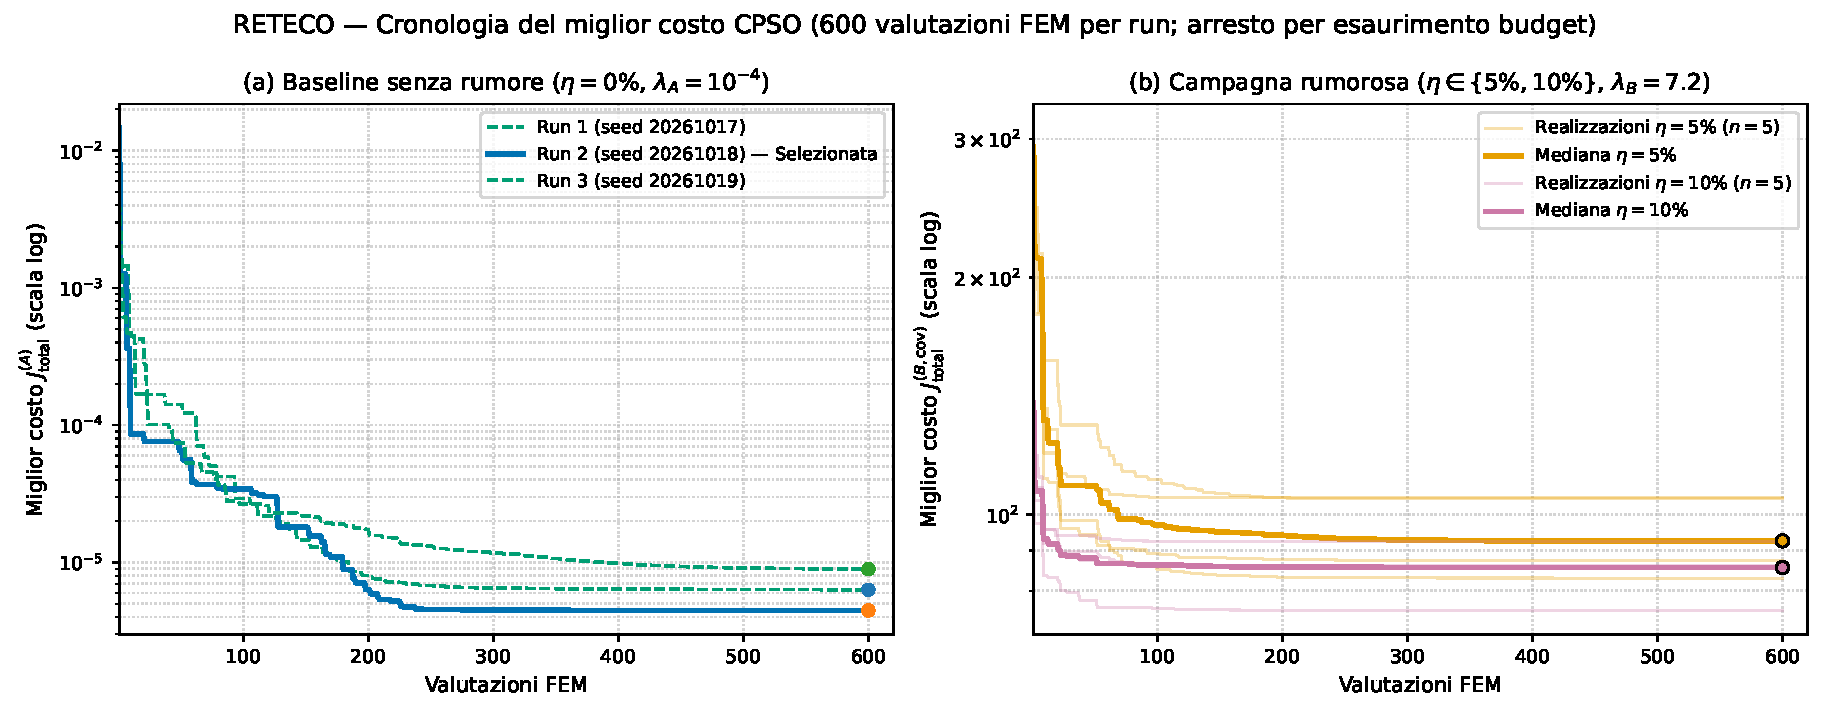
\includegraphics[width=0.98\textwidth,trim=0pt 0pt 0pt 25pt,clip]{paper/fig07_final_cpso_convergence.pdf}
\caption{Cronologia del miglior valore osservato del funzionale obiettivo durante le valutazioni FEM. Il pannello (a) mostra le tre run della baseline senza rumore con pesatura deterministica (Mode A); il pannello (b) mostra le dieci run rumorose con pesatura a covarianza inversa (Mode B covariance), insieme alle mediane empiriche per livello. Le ordinate hanno scale distinte e rappresentano funzionali pesati diversi: i valori assoluti tra pannelli e tra livelli di rumore non sono direttamente confrontabili. Tutte le run terminano per esaurimento del budget; un plateau della curva non costituisce, da solo, una certificazione di convergenza. Il ritaglio LaTeX rimuove soltanto l'intestazione interna con il nome del progetto; il PDF sorgente non è stato modificato.}
\label{fig:cpso-final-convergence}
\end{figure*}
\FloatBarrier

\subsection{Interpretazione della pesatura e limiti della campagna}

La diagnostica dei modi di pesatura conferma che la normalizzazione del termine dati interagisce con $\lambda$. Per il parametro vero sintetico e il livello nominale del 10\%, il termine $J_{\rm data}$ vale $4.119\times10^{-3}$ con la pesatura deterministica, $0.4119$ con la pesatura noise-weighted mean e $74.144$ con la covarianza inversa esatta. Questi valori sono una verifica di scala del funzionale, non una comparazione di prestazioni dell'ottimizzatore. Non è stata eseguita una campagna comparativa a budget equivalente con altri algoritmi; il manoscritto non rivendica quindi superiorità del CPSO.

\FloatBarrier

\section{Conclusioni}
\label{sec:conclusions}
Il lavoro ha formulato e implementato un modello ridotto Biot--Darcy con una legge di Kelvin--Voigt frazionaria per la matrice e un tracciante passivo con accumulo frazionario. Le verifiche MMS mostrano errori decrescenti e ordini spaziali osservati prossimi a quelli attesi per lo spostamento in $L^2$ e per pressione e concentrazione; tuttavia, la serie coordinata non isola completamente l'errore spaziale del tracciante e non sostituisce un'analisi teorica completa dell'errore né una verifica inf--sup. I test di massa raggiungono drift dell'ordine della precisione macchina, mentre l'identità algebrica passo-passo e il residuo energetico cumulativo sono stati trattati come controlli distinti.

La mesh quadrilatera derivata da una sezione BraTS 2020 riproduce con elevata sovrapposizione la maschera adottata, ma il dominio è un proxy del parenchima, non una segmentazione tissutale specifica della sostanza bianca. Le sorgenti e i campi temporali della dimostrazione anatomica sono sintetici; non sono disponibili osservazioni cliniche longitudinali che consentano di validare le traiettorie o di interpretare le stime come parametri fisiologici.

L'analisi del Jacobiano discreto conferma la degenerazione prevista quando il flusso è nullo e mostra rango pieno locale nel protocollo attivo. I profili ottimizzati indicano che il valore preferito di $\beta$ dipende dalla componente del funzionale considerata: il minimo campionato del termine dati è in $0.45$, mentre quello del funzionale regolarizzato è in circa $0.479$. Il profilo dati è inoltre sensibile alla discretizzazione inversa: passando da $(N,M)=(16,80)$ a $(24,120)$ il minimo campionato si sposta a $0.4375$ e il valore minimo del profilo diminuisce. Queste osservazioni sono coerenti con una valle di costo piatta e con un effetto non trascurabile del prior, ma non dimostrano da sole non-identificabilità strutturale di $\beta$ nel protocollo attivo.

La campagna finale comprende tre run senza rumore e dieci run rumorose con budget pianificato di 600 valutazioni FEM. La dispersione delle stime è contenuta per alcuni parametri nei campioni osservati, ma resta marcata per $\beta$ ed $E$; gli errori non variano monotonicamente con il livello nominale di rumore. Tutte le esecuzioni hanno esaurito il budget senza certificare convergenza, e le dieci run rumorose condividono lo stesso seed CPSO. I dati supportano quindi una caratterizzazione controllata del problema inverso sintetico, non una dimostrazione generale di robustezza dell'algoritmo.

Prima della sottomissione occorre completare almeno quattro verifiche: (i) estendere la sensibilità della discretizzazione e del passo temporale, separando gli errori del forward solver da quelli di ottimizzazione; (ii) aumentare le repliche e incrociare seed del rumore e seed CPSO per quantificare entrambe le fonti di variabilità; (iii) confrontare eventuali ottimizzatori alternativi a parità di funzione obiettivo, discretizzazione e budget, se si intendono formulare affermazioni comparative; (iv) depositare un archivio versionato che permetta di rigenerare ogni tabella e figura. Un'applicazione clinica alla sostanza bianca richiederebbe inoltre una segmentazione tissutale indipendente e osservazioni adeguate per la validazione. In assenza di tali dati, la conclusione appropriata è quella di una verifica numerica e metodologica preliminare, con limiti esplicitati.


\FloatBarrier
\section*{Disponibilità di dati e codice}
Il codice del solutore e le configurazioni dei protocolli sono conservati nel repository \href{https://github.com/GiovanniIacuzzo/Fractional-Poro-Viscoelastic}{\texttt{Fractional-Poro-Viscoelastic}}. La revisione del codice consultata per questo articolo e gli identificativi degli esperimenti sono riportati in Appendice~\ref{app:repro}. Le immagini MRI e le annotazioni del caso BraTS provengono dalla distribuzione BraTS 2020~\citep{brats2020protocol}. Le osservazioni longitudinali del tracciante sono sintetiche. Le tabelle riportano le stime e le numerosità delle campagne analizzate.

\bibliographystyle{unsrtnat}
\bibliography{references}
\clearpage
\onecolumn
\appendix
\renewcommand{\thefigure}{\thesection.\arabic{figure}}
\renewcommand{\thetable}{\thesection.\arabic{table}}
\renewcommand{\theequation}{\thesection.\arabic{equation}}
\renewcommand{\theHfigure}{app.\thesection.\arabic{figure}}
\renewcommand{\theHtable}{app.\thesection.\arabic{table}}
\renewcommand{\theHequation}{app.\thesection.\arabic{equation}}
\section{Tabelle complete di convergenza e diagnostiche MMS}
\label{app:mms}

\subsection{Raffinamento spaziale}

La Tabella~\ref{tab:spatial-full} riporta gli errori $L^2$ e $H^1$ della serie coordinata. Lo spostamento è approssimato con elementi quadratici, mentre pressione e tracciante usano elementi lineari. Il tasso $H^1$ del tracciante non risulta ancora stabilizzato; inoltre, il raffinamento temporale coordinato con quello spaziale implica che gli EOC osservati non isolano completamente l'errore spaziale.

\begin{table*}[!t]
\centering
\caption{Errori MMS spaziali completi. Gli EOC sono calcolati tra livelli consecutivi; $h=1/N$ indica la larghezza della cella quadrata.}
\label{tab:spatial-full}
\scriptsize
\begin{tabular}{c|cc|cc|cc}
\toprule
$h=1/N$ & $\|e_d\|_{L^2}$ & $\|e_d\|_{H^1}$ & $\|e_p\|_{L^2}$ & $\|e_p\|_{H^1}$ & $\|e_c\|_{L^2}$ & $\|e_c\|_{H^1}$\\
\midrule
0.2500 & $2.6870\cdot10^{-3}$ & $7.2341\cdot10^{-2}$ & $5.4526\cdot10^{-3}$ & $1.2690\cdot10^{-1}$ & $2.4562\cdot10^{-2}$ & $1.2535\cdot10^{-1}$\\
0.1250 & $3.5294\cdot10^{-4}$ & $1.8383\cdot10^{-2}$ & $1.3055\cdot10^{-3}$ & $6.3093\cdot10^{-2}$ & $6.3959\cdot10^{-3}$ & $3.8283\cdot10^{-2}$\\
0.0625 & $4.4932\cdot10^{-5}$ & $4.6130\cdot10^{-3}$ & $3.2286\cdot10^{-4}$ & $3.1496\cdot10^{-2}$ & $1.6164\cdot10^{-3}$ & $1.4518\cdot10^{-2}$\\
\midrule
EOC $0.25\to0.125$ & 2.93 & 1.98 & 2.06 & 1.01 & 1.94 & 1.71\\
EOC $0.125\to0.0625$ & 2.97 & 1.99 & 2.02 & 1.00 & 1.98 & 1.40\\
\bottomrule
\end{tabular}
\end{table*}
\FloatBarrier

\subsection{Raffinamento temporale e bilanci}

\begin{table*}[!t]
\centering
\caption{Errori $L^2$ e tassi temporali osservati con spazio FEM fissato $Q_2/Q_2/Q_2$.}
\label{tab:temporal-full}
\small
\begin{tabular}{c|cc|cc|cc}
\toprule
$\Delta t_{\max}$ & $\|e_d\|_{L^2}$ & EOC$_t$ & $\|e_p\|_{L^2}$ & EOC$_t$ & $\|e_c\|_{L^2}$ & EOC$_t$\\
\midrule
0.05000 & $1.3569\cdot10^{-3}$ & -- & $2.7205\cdot10^{-2}$ & -- & $1.3713\cdot10^{-1}$ & --\\
0.02500 & $6.3341\cdot10^{-4}$ & 1.10 & $1.3843\cdot10^{-2}$ & 0.97 & $7.0004\cdot10^{-2}$ & 0.97\\
0.01250 & $3.0010\cdot10^{-4}$ & 1.08 & $6.9863\cdot10^{-3}$ & 0.99 & $3.5421\cdot10^{-2}$ & 0.98\\
0.00625 & $1.4436\cdot10^{-4}$ & 1.06 & $3.5106\cdot10^{-3}$ & 0.99 & $1.7835\cdot10^{-2}$ & 0.99\\
\bottomrule
\end{tabular}
\end{table*}
\FloatBarrier

\begin{table}[!htbp]
\centering
\caption{Residuo energetico cumulativo finale al variare del passo massimo sul dominio unitario.}
\label{tab:energy-dt}
\small
\begin{tabular}{cc}
\toprule
$\Delta t$ & $|R_N|$\\
\midrule
0.040 & $2.0739\cdot10^{-3}$\\
0.020 & $1.1042\cdot10^{-3}$\\
0.010 & $5.7074\cdot10^{-4}$\\
0.005 & $2.9028\cdot10^{-4}$\\
\bottomrule
\end{tabular}
\end{table}
\FloatBarrier

La massa passa da $M(0)=0.1628317137332642$ a $M(T)=0.1628317137332636$, con drift relativo $3.92\times10^{-15}$. Il residuo di compatibilità iniziale è $5.45\times10^{-16}$ e l'errore massimo dell'identità algebrica al passo è $4.78\times10^{-17}$. Tali valori descrivono i casi eseguiti e non costituiscono una dimostrazione generale della stabilità energetica dello schema discreto.

\begin{figure*}[!t]
\centering
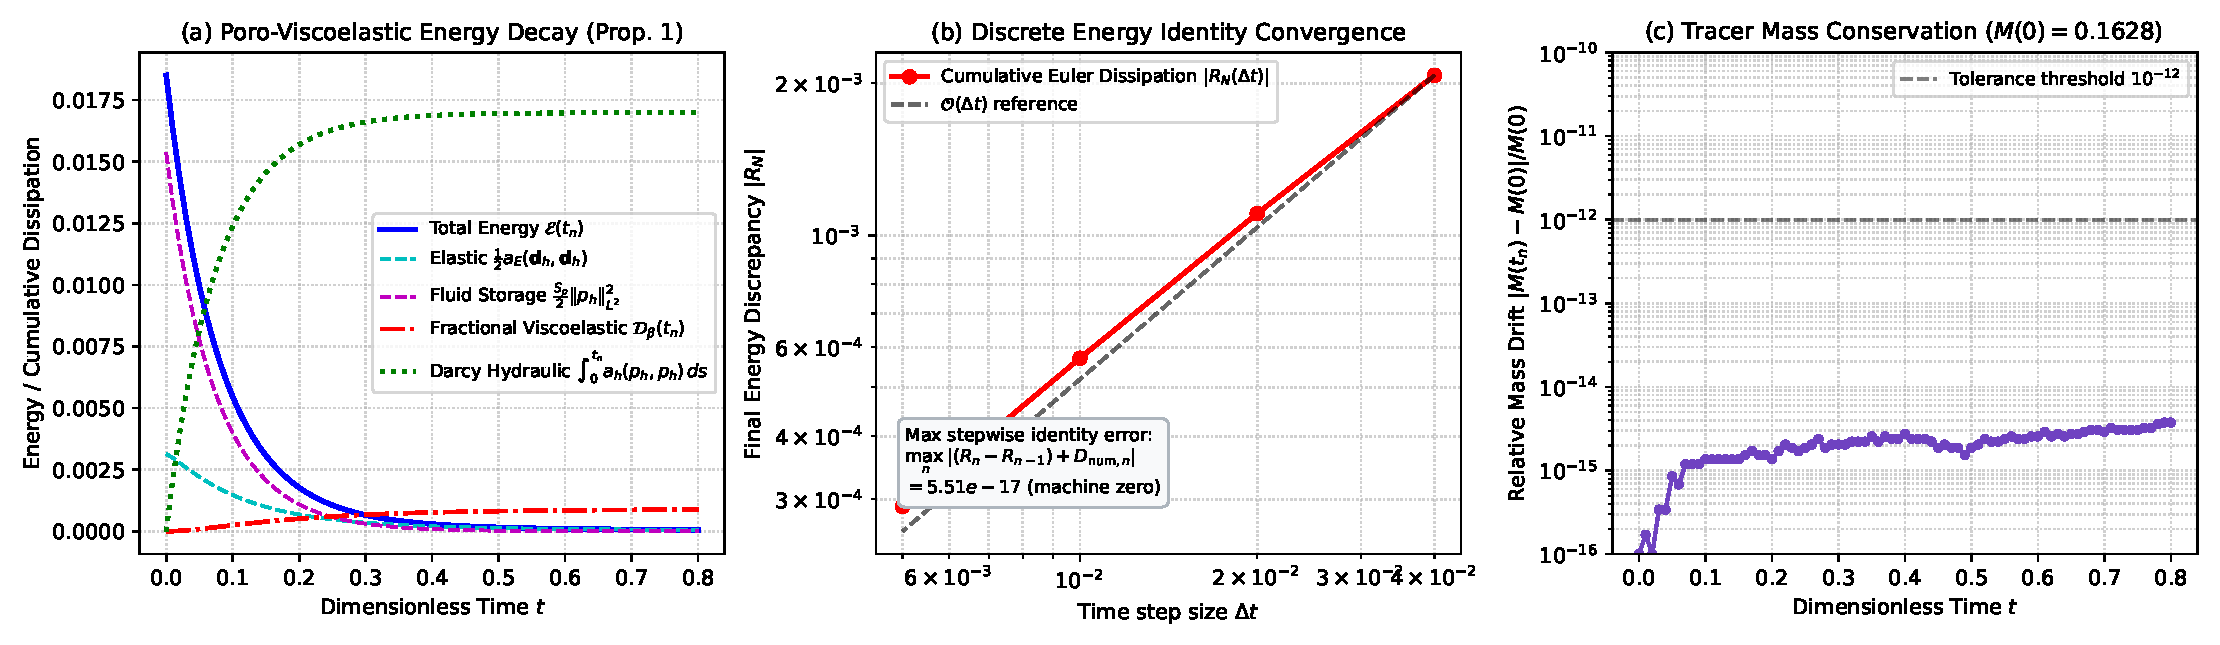
\includegraphics[width=0.78\textwidth]{appendices/figs_01_energy_and_mass_conservation.pdf}
\caption{Diagnostiche di energia e massa sul dominio MMS unitario. Questa prova è distinta dal caso anatomico forzato.}
\label{fig:app-mms-energy}
\end{figure*}

\begin{figure*}[!t]
\centering
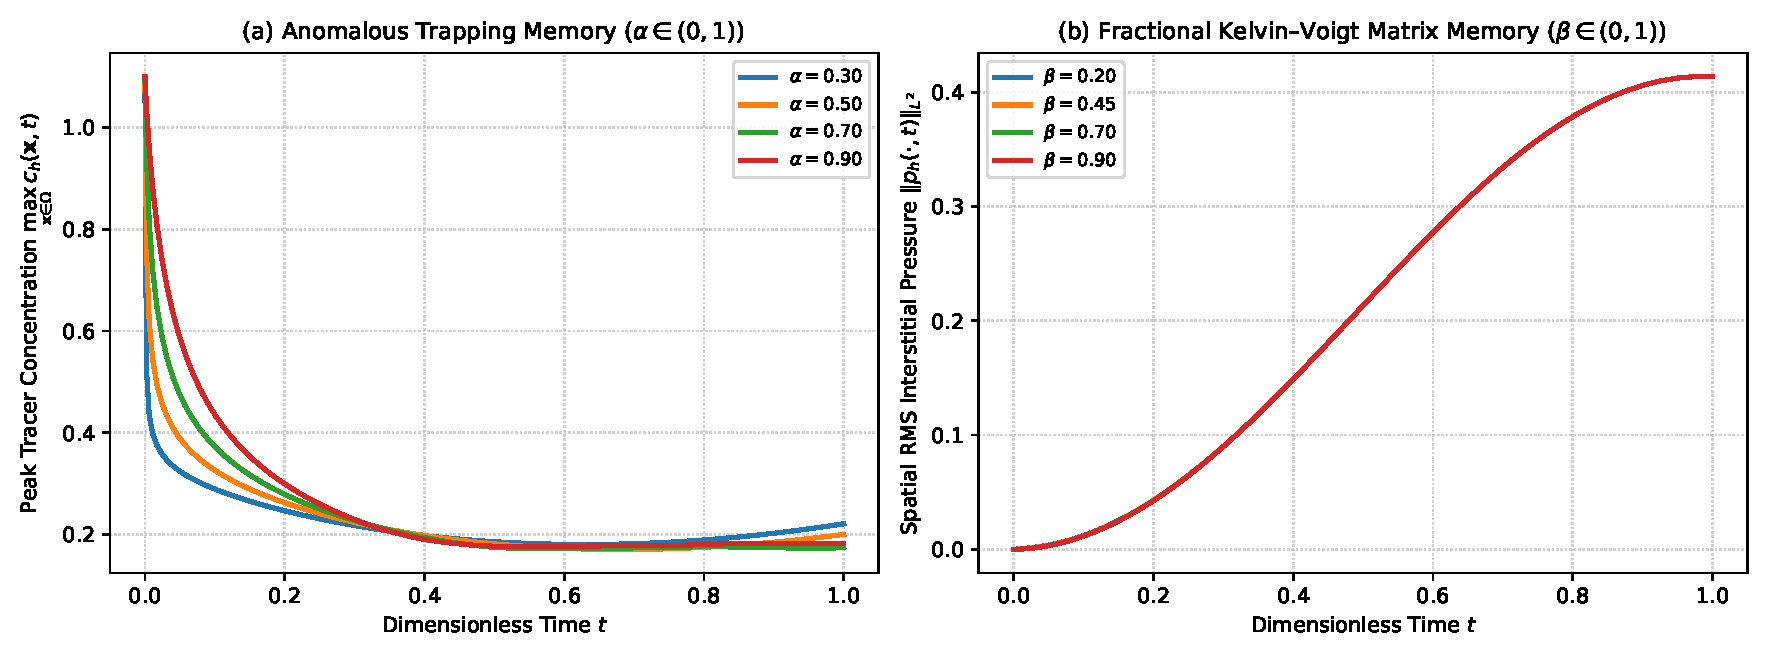
\includegraphics[width=0.78\textwidth]{appendices/figs_02_fractional_orders_physics_sensitivity.pdf}
\caption{Sensibilità delle traiettorie agli ordini frazionari sul dominio unitario. Il grafico è diagnostico e non dimostra, da solo, identificabilità dei parametri.}
\label{fig:app-mms-fractional}
\end{figure*}

\FloatBarrier
\section{Geometria anatomica e sensibilità della simulazione}
\label{app:anatomy}

La geometria deriva dalla sezione assiale $k=67$ del soggetto \texttt{BraTS20\_Training\_001}. I volumi sono orientati in RAS+ con spacing isotropo di 1 mm; il report registra 202 facce di bordo, area della maschera pari a $17069\,\mathrm{mm}^2$, area della mesh pari a $17068.288\,\mathrm{mm}^2$, Dice 0.998155 e IoU 0.996317. La maschera è un proxy del parenchima: le label BraTS descrivono sottoregioni tumorali e non forniscono una segmentazione della sostanza bianca.

\subsection{Evoluzione temporale e sensibilità alla discretizzazione}

\begin{figure*}[!t]
\centering
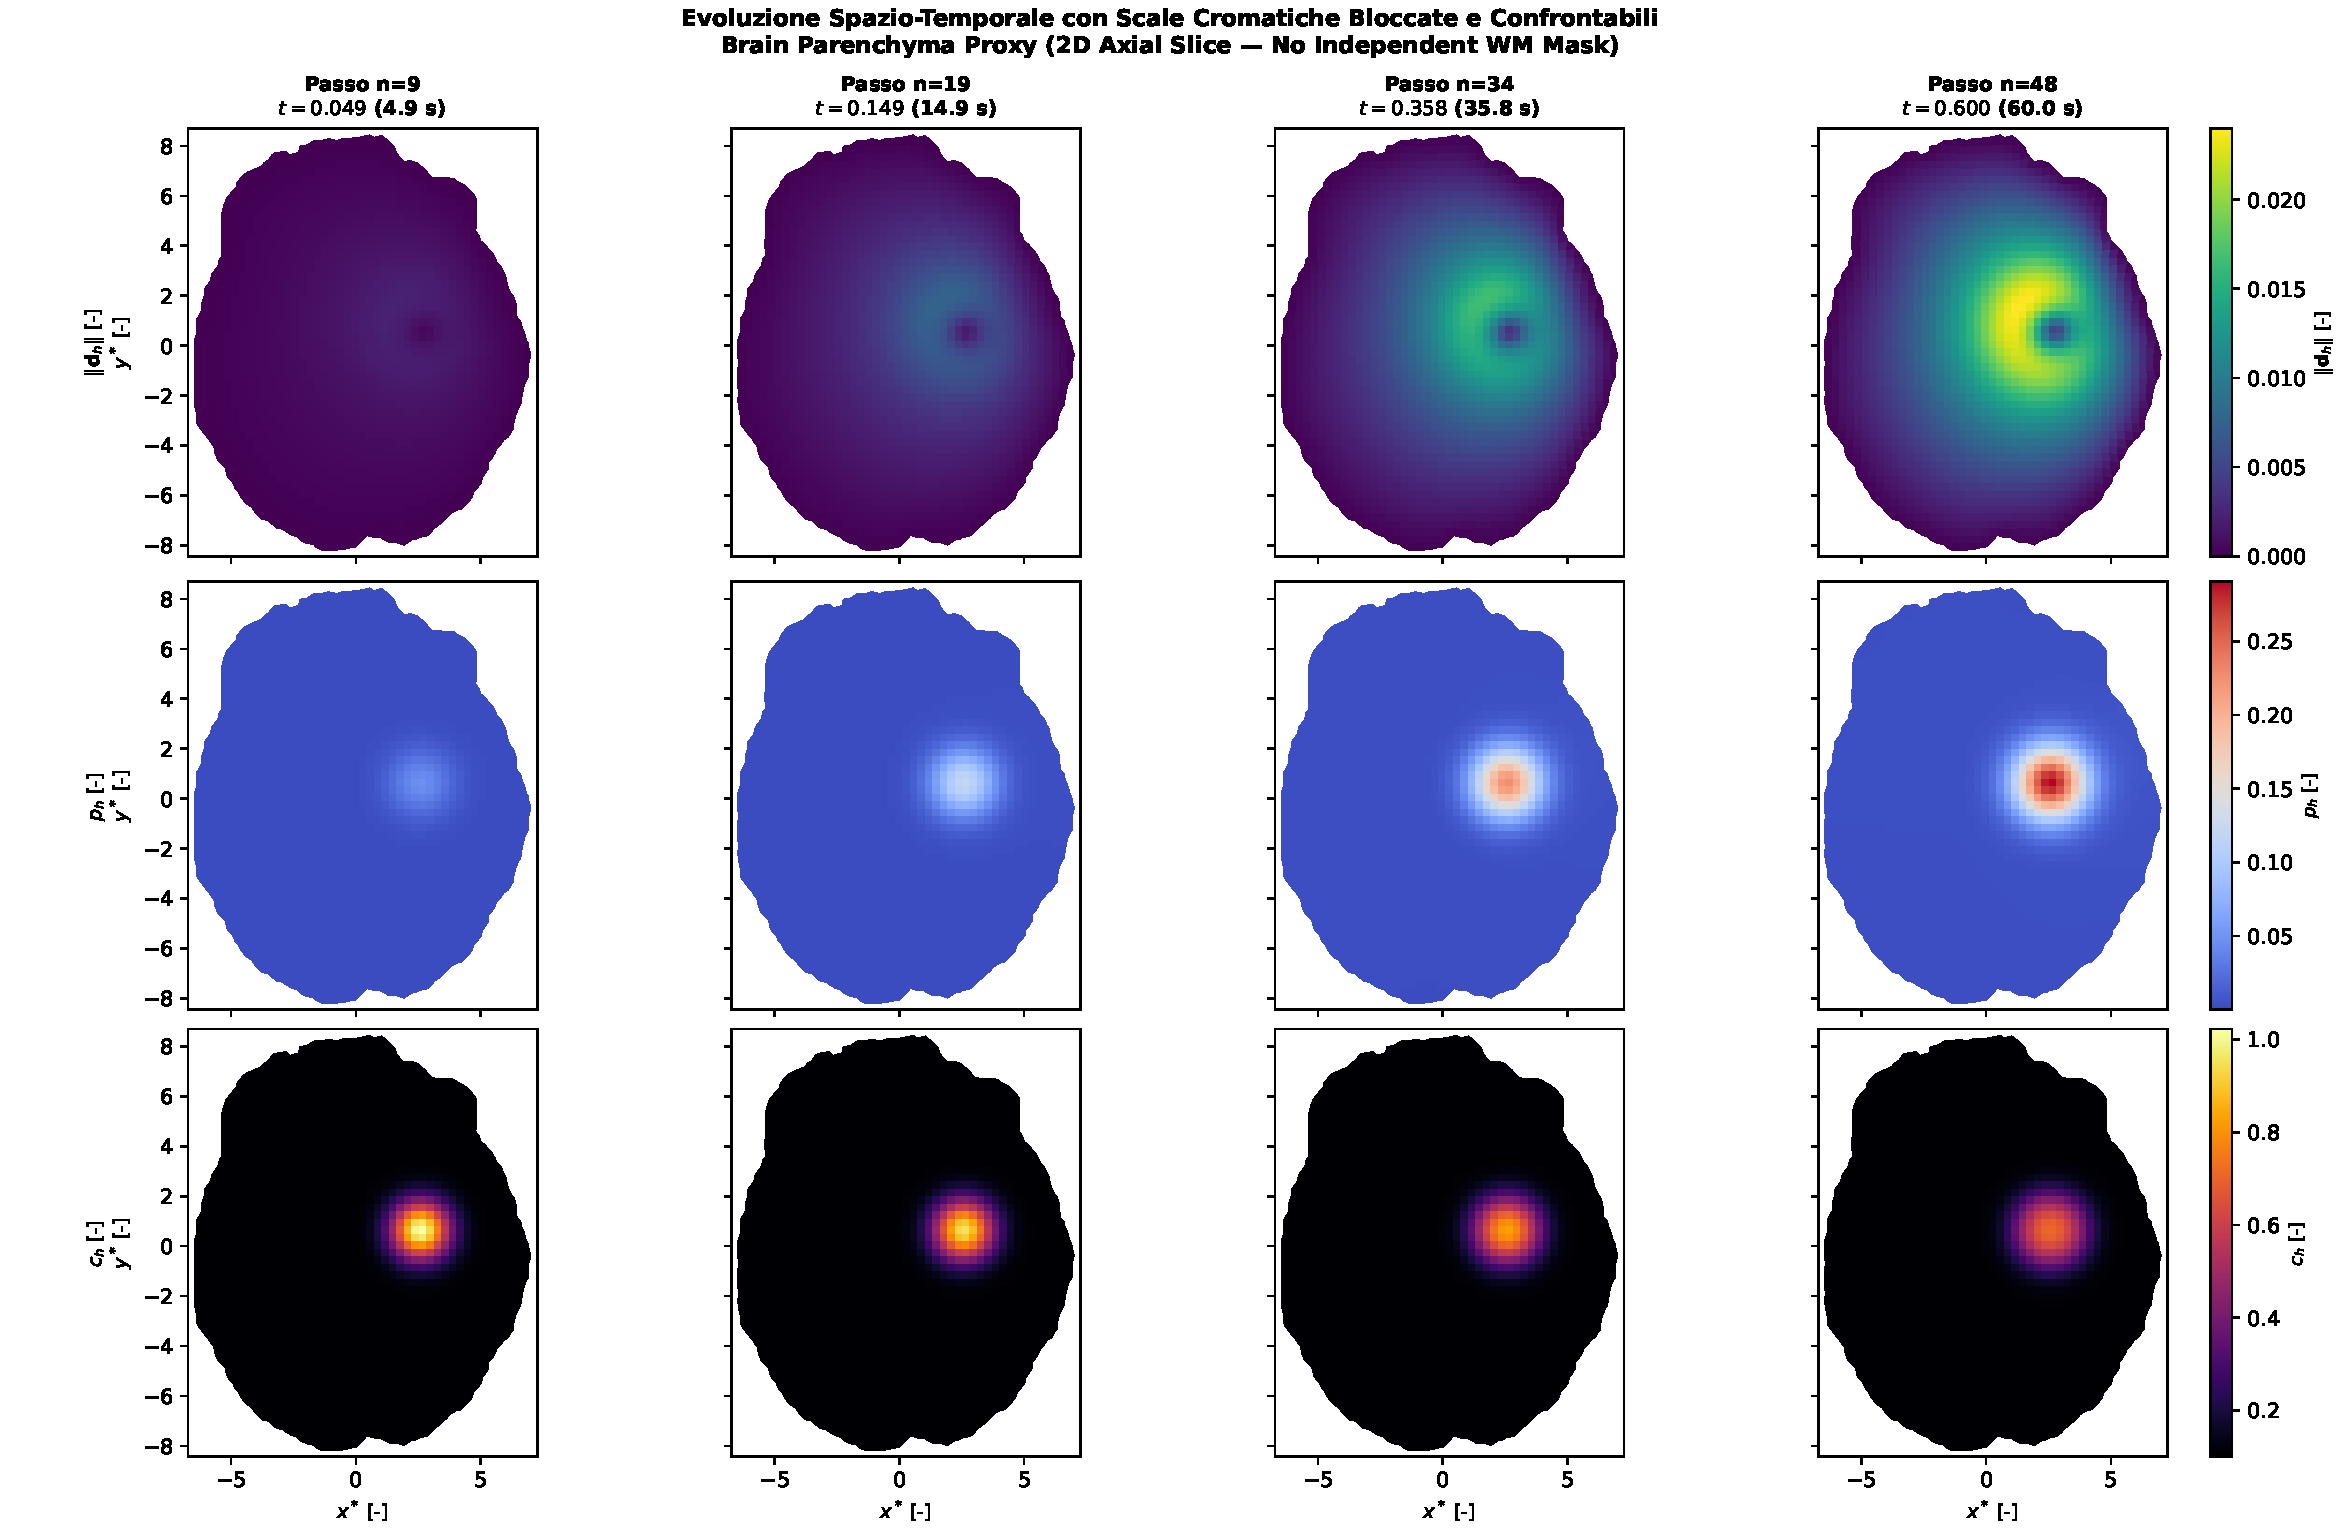
\includegraphics[width=\textwidth]{appendices/figs_07_temporal_evolution_comparable_scales.pdf}
\caption{Evoluzione temporale dei campi sul dominio anatomico. Gli stati sono simulati e dipendono dalle forzanti sintetiche specificate nel testo.}
\label{fig:app-anatomical-time}
\end{figure*}

\begin{figure*}[!t]
\centering
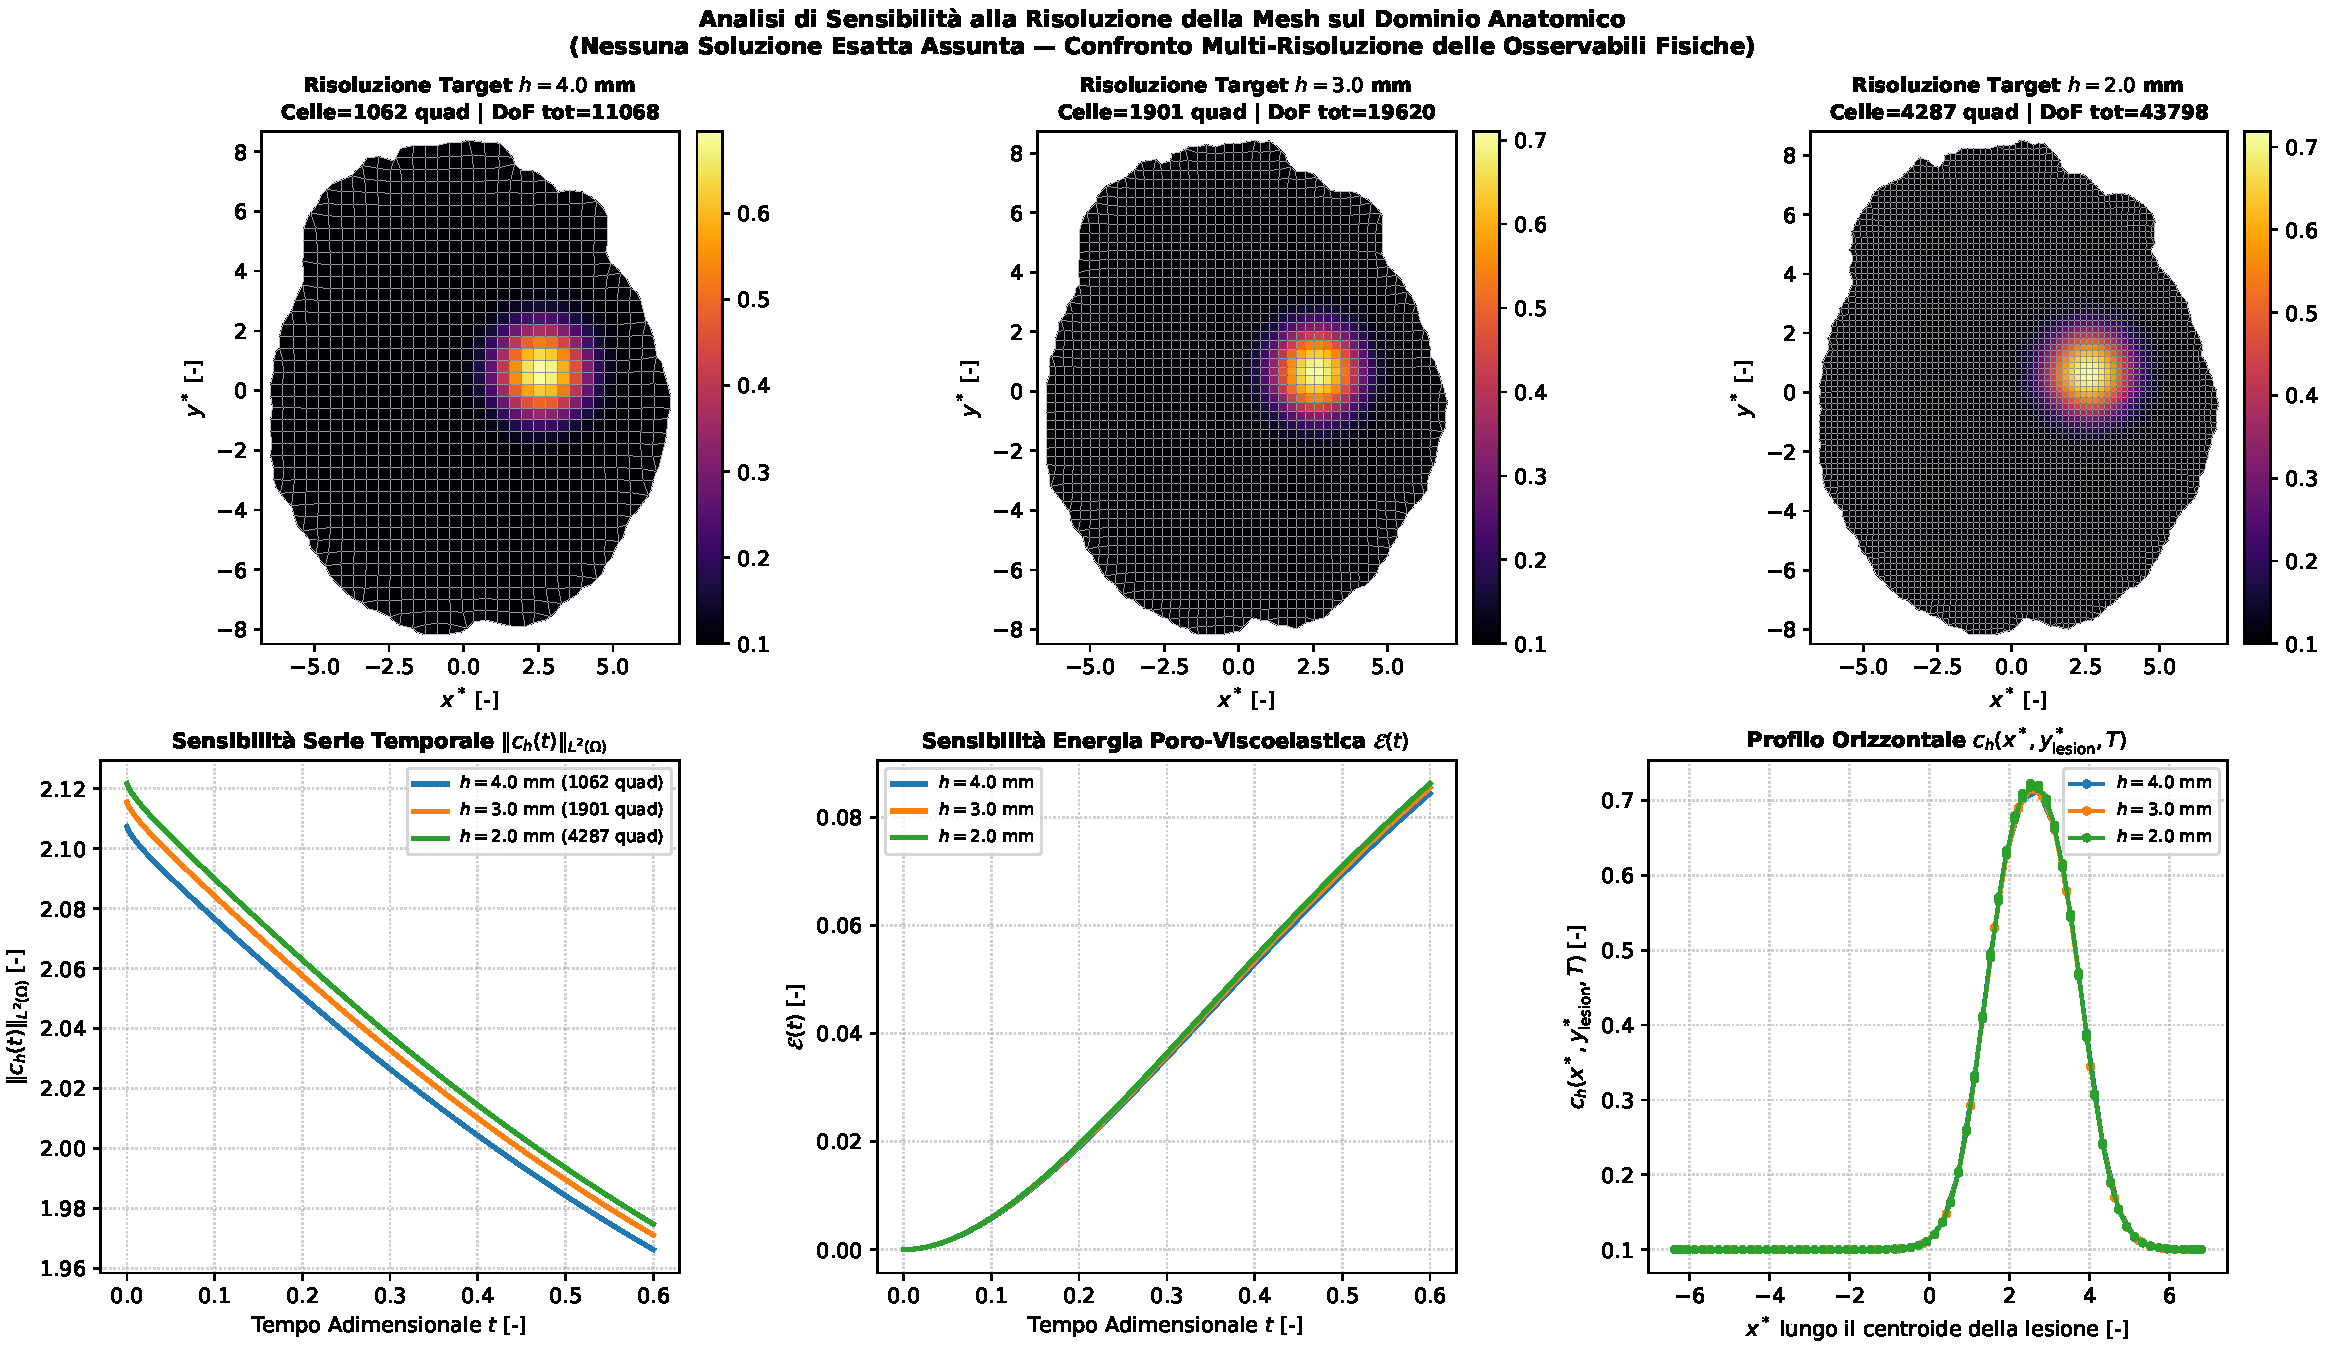
\includegraphics[width=\textwidth]{appendices/figs_08_mesh_resolution_sensitivity.pdf}
\caption{Confronto delle mesh con lati obiettivo pari a 4, 3 e 2 mm. Le differenze rispetto alla mesh più fine sono indicatori di sensibilità alla discretizzazione, non ordini asintotici.}
\label{fig:app-mesh-sensitivity}
\end{figure*}
\FloatBarrier

\subsection{Sensibilità agli ordini frazionari}

\begin{figure*}[!t]
\centering
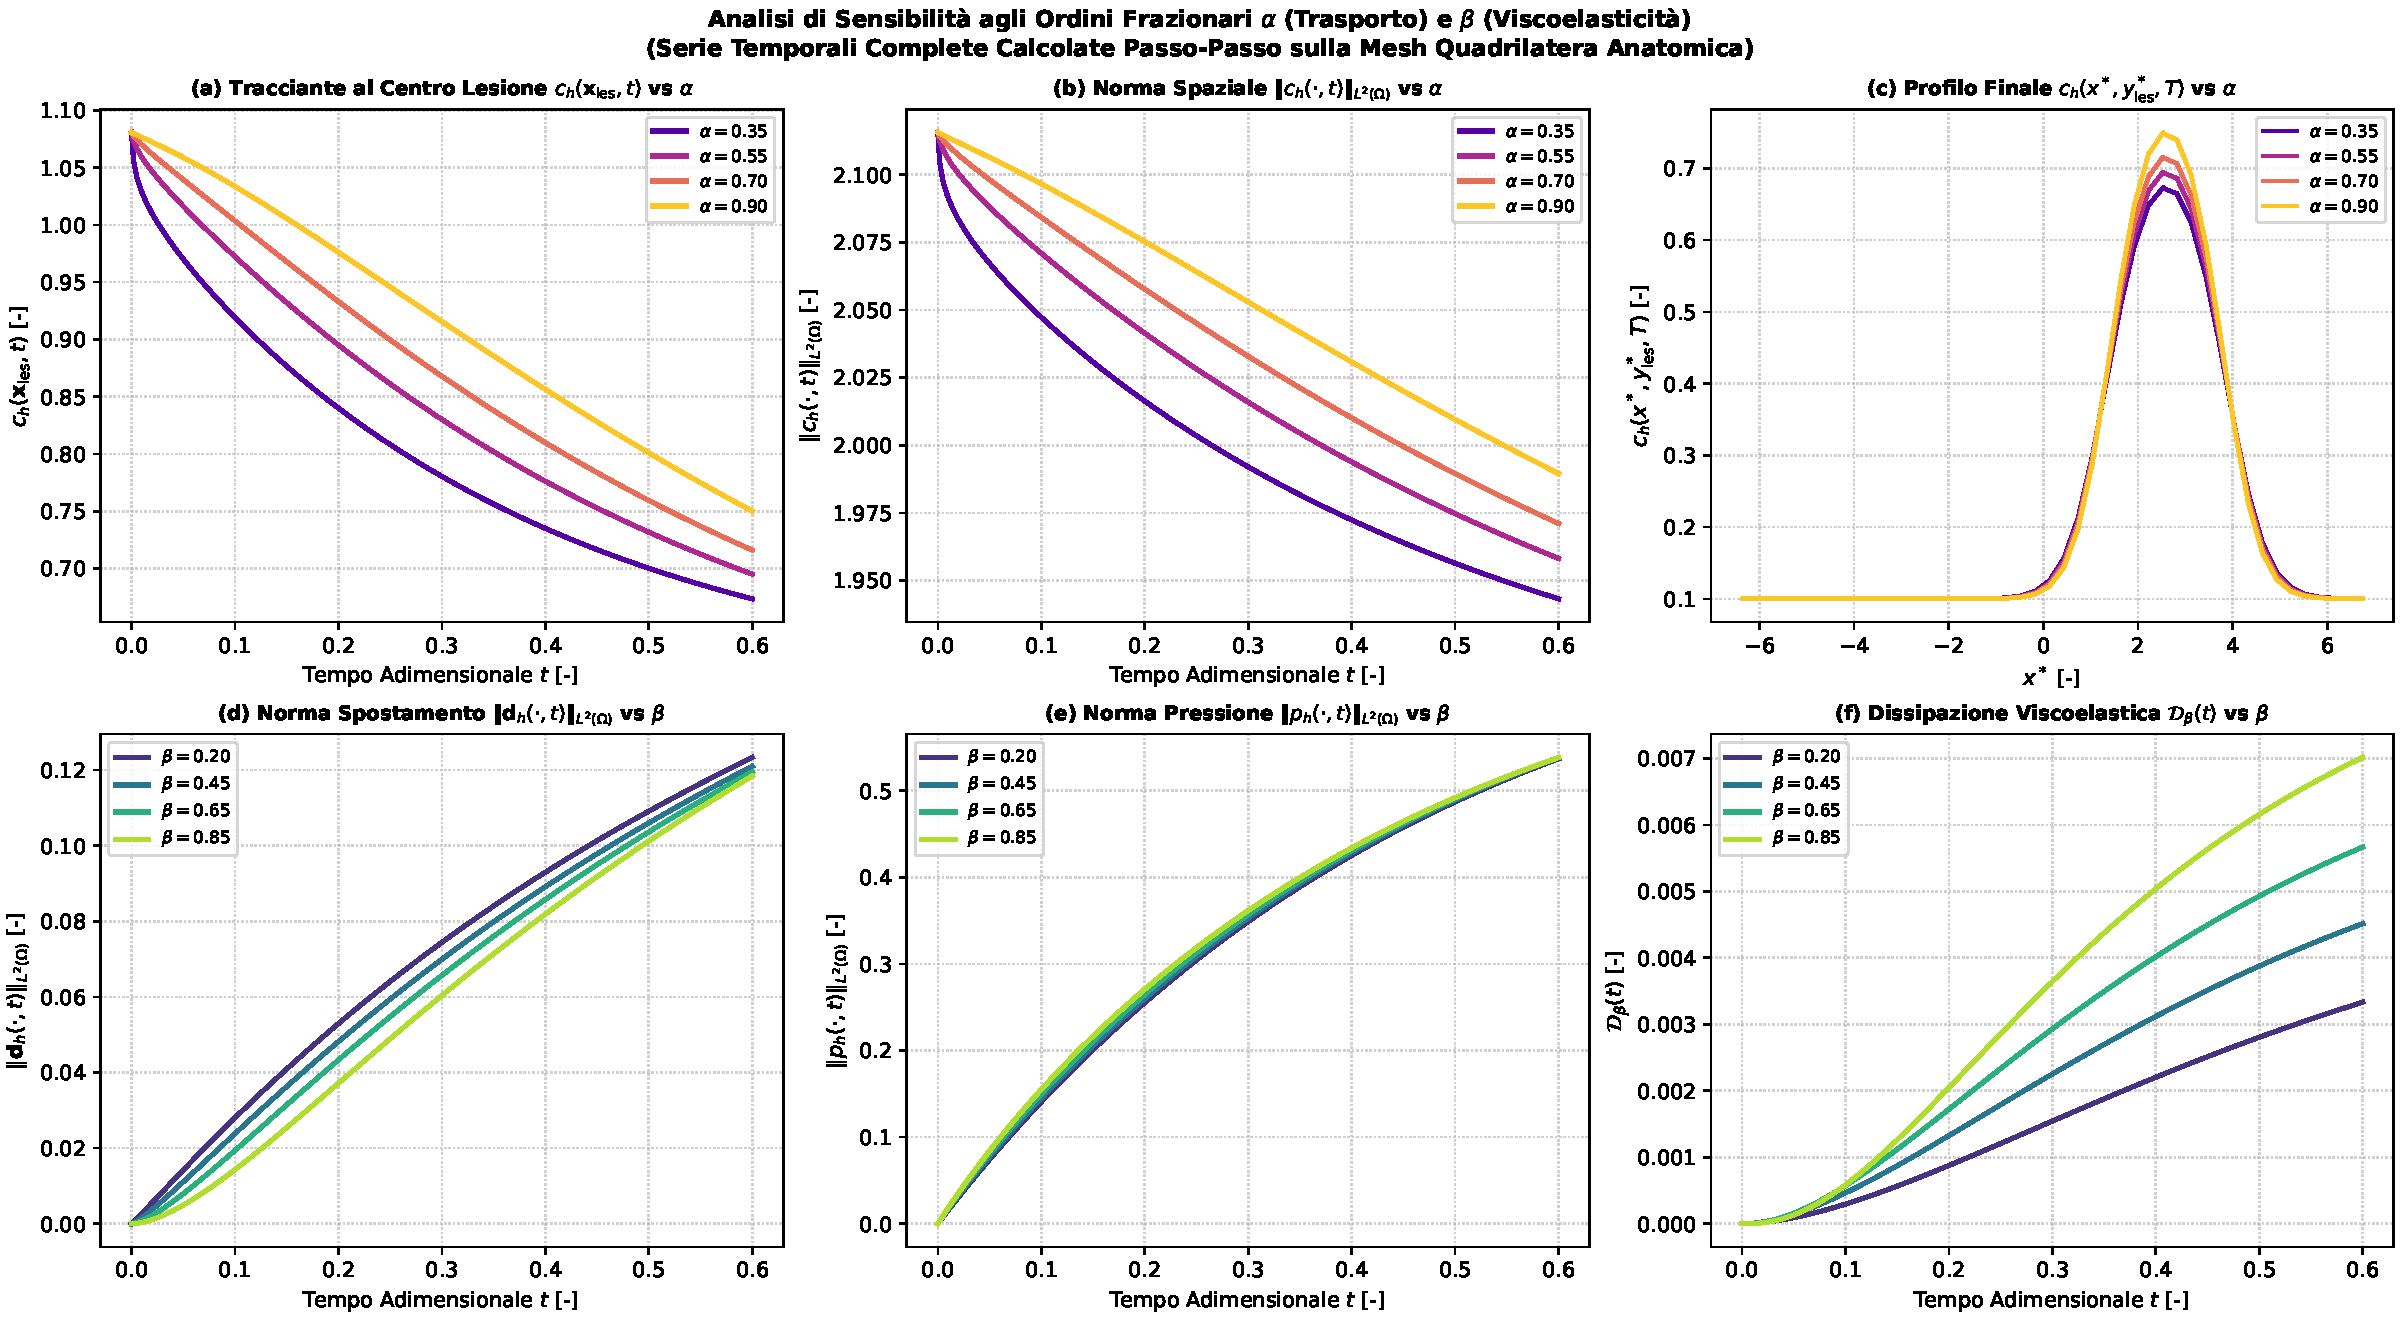
\includegraphics[width=\textwidth]{appendices/figs_09_fractional_parameters_sensitivity.pdf}
\caption{Sensibilità delle quantità di stato a $\alpha$ e $\beta$ nel protocollo anatomico sintetico. Le curve descrivono la risposta del forward model e non costituiscono una prova autonoma di identificabilità.}
\label{fig:app-anatomical-fractional}
\end{figure*}

\FloatBarrier
\section{Identificabilità locale e geometria del funzionale}
\label{app:identifiability}
\setcounter{figure}{0}
\setcounter{table}{0}
\setcounter{equation}{0}

L'operatore osservativo impiegato nelle campagne inverse campiona la sola concentrazione in $36$ sensori a cinque istanti, per un totale di $180$ osservazioni adimensionali. In questa diagnostica si usano pesi identità, che definiscono una metrica geometrica sulle osservazioni.

\subsection{Confronto del Jacobiano tra flusso nullo e attivo}

La Tabella~\ref{tab:app-jacobian} sintetizza le diagnostiche spettrali del Jacobiano discreto della mappa osservativa rispetto ai parametri normalizzati $\widetilde{\boldsymbol{\theta}}=(\widetilde{\alpha},\widetilde{\beta},\widetilde{D},\widetilde{E})$ nei regimi a flusso di Darcy nullo e attivo. La Figura~\ref{fig:app-flow-svd-comparison} visualizza il confronto tra sensibilità e spettro singolare; la Figura~\ref{fig:app-local-geometry} descrive invece la geometria locale delle correlazioni e delle similarità tra colonne.

\begin{table}[H]
\centering
\caption{Diagnostiche locali del Jacobiano discreto della mappa osservativa rispetto a $(\alpha,\beta,D,E)$ nelle coordinate normalizzate. Il rango e il numero di condizionamento sono riferiti al punto di linearizzazione e alla soglia numerica adottata.}
\label{tab:app-jacobian}
\small
\setlength{\tabcolsep}{8pt}
\begin{tabular}{@{}p{0.32\textwidth}p{0.28\textwidth}p{0.32\textwidth}@{}}
\toprule
Diagnostica & Flusso nullo ($\mathbf{q} \equiv \mathbf{0}$) & Flusso attivo ($\mathbf{q} \neq \mathbf{0}$) \\
\midrule
Rango numerico                        & $2$ su $4$                     & $4$ su $4$ \\
Valori singolari                      & $(1.5833,\,0.3222,\,0,\,0)$    & $(1.2261,\,0.3619,\,0.2924,\,0.04949)$ \\
Colonne identicamente nulle           & $\widetilde{\beta}$ ed $\widetilde{E}$ & nessuna nel punto testato \\
Numero di condizionamento             & non definito (rango deficitario) & $24.78$ \\
Massimo flusso di Darcy al riferimento & $0$                            & $0.05737$ \\
Schema alle differenze finite centrate & passo $10^{-4}$                & passo $10^{-4}$ \\
\bottomrule
\end{tabular}
\end{table}

Nel regime a flusso nullo, nove traiettorie di verifica hanno restituito campi meccanici e idraulici nulli entro la tolleranza numerica; la concentrazione risulta indipendente da $E$ e $\beta$ come previsto dall'equazione del tracciante. Per il protocollo attivo di riferimento, il Jacobiano ha spettro $(1.2261,0.3619,0.2924,0.04949)$ e numero di condizionamento $24.78$. La scansione della sottosezione seguente mostra come il valore singolare minimo e il condizionamento variano quando il livello di eccitazione viene modificato.

\begin{figure*}[t]
\centering
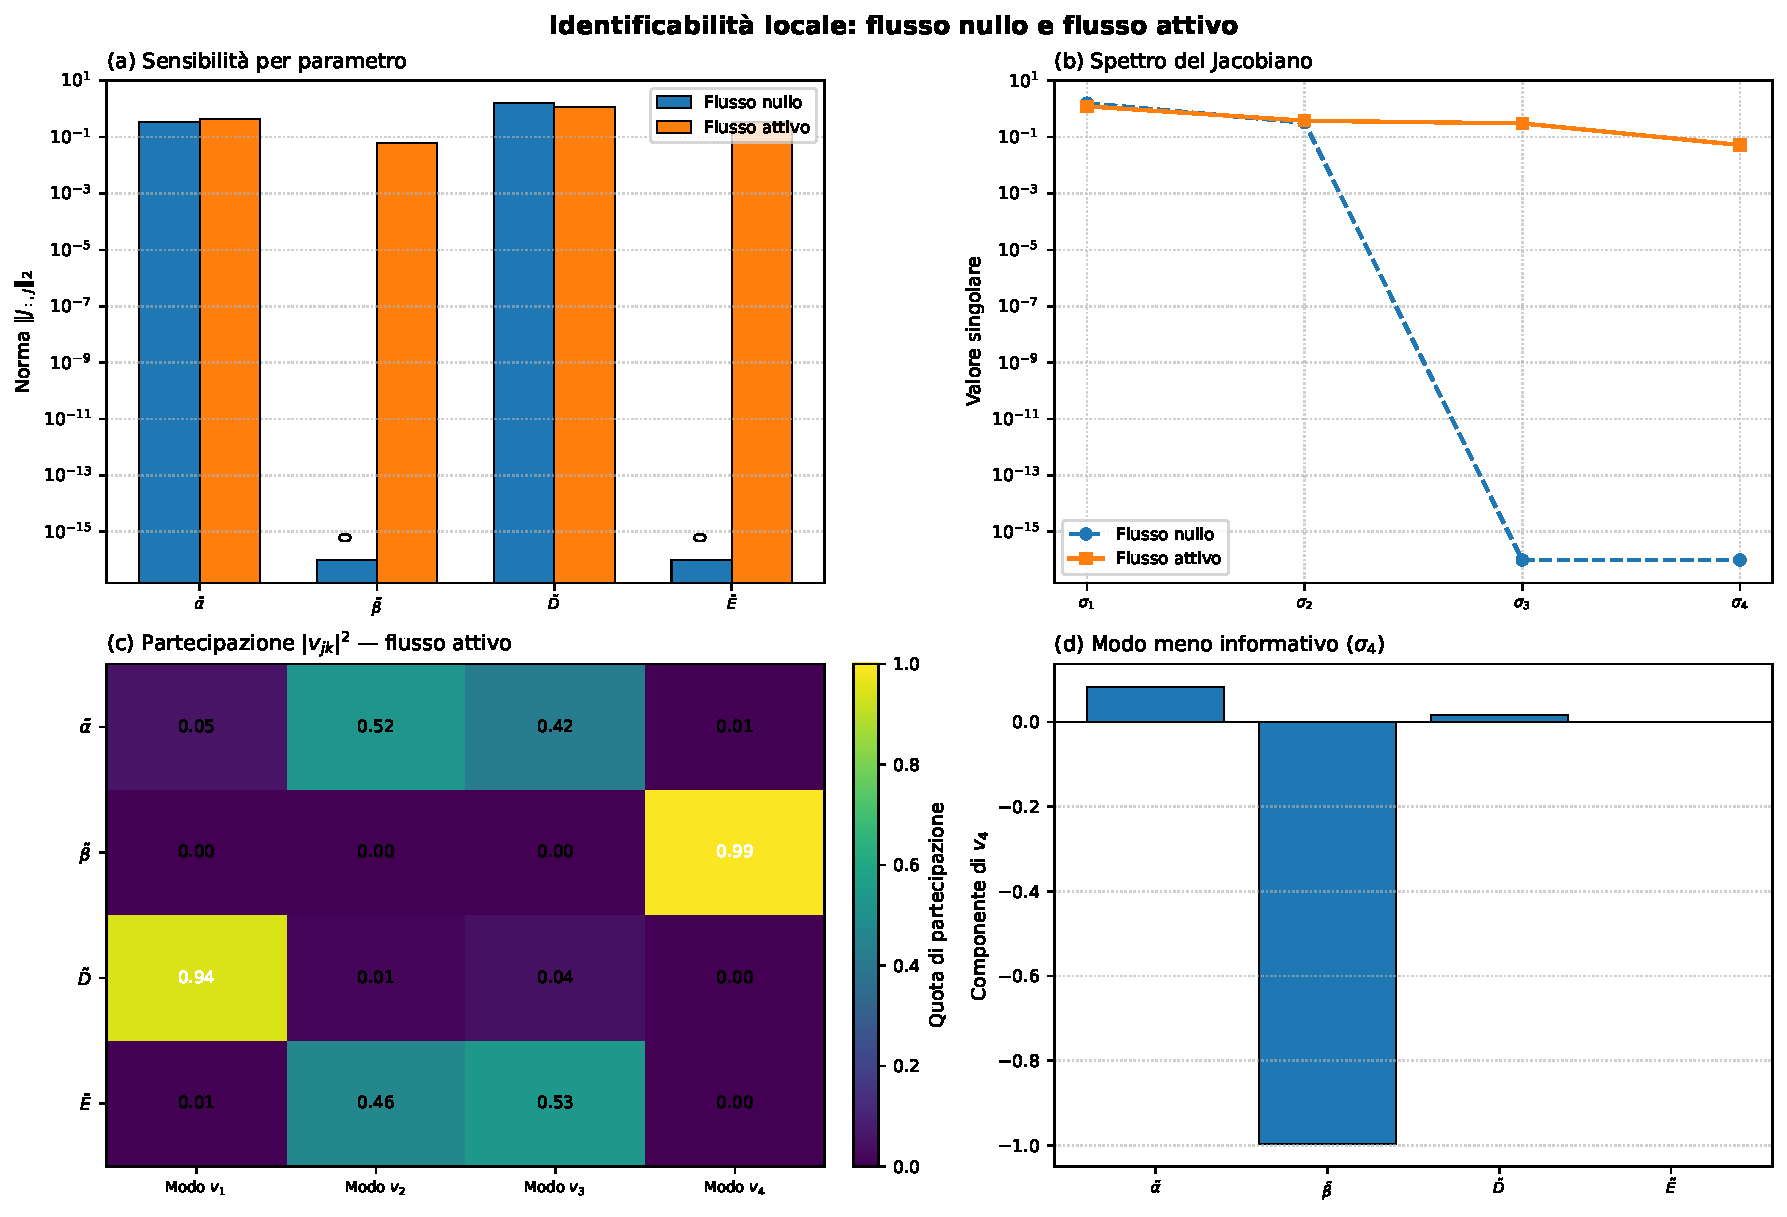
\includegraphics[width=0.85\textwidth]{appendices/figs_C01_local_svd_flow_comparison.pdf}
\caption{Confronto del Jacobiano osservativo a flusso nullo e attivo sul quadrato unitario. Il flusso nullo produce due colonne nulle ($\widetilde\beta$ e $\widetilde E$) e due valori singolari nulli; nel caso attivo, il modo singolare meno informativo resta dominato da $\widetilde\beta$. I pesi sono identità sulle osservazioni adimensionali.}
\label{fig:app-flow-svd-comparison}
\end{figure*}

\begin{figure}[H]
\centering
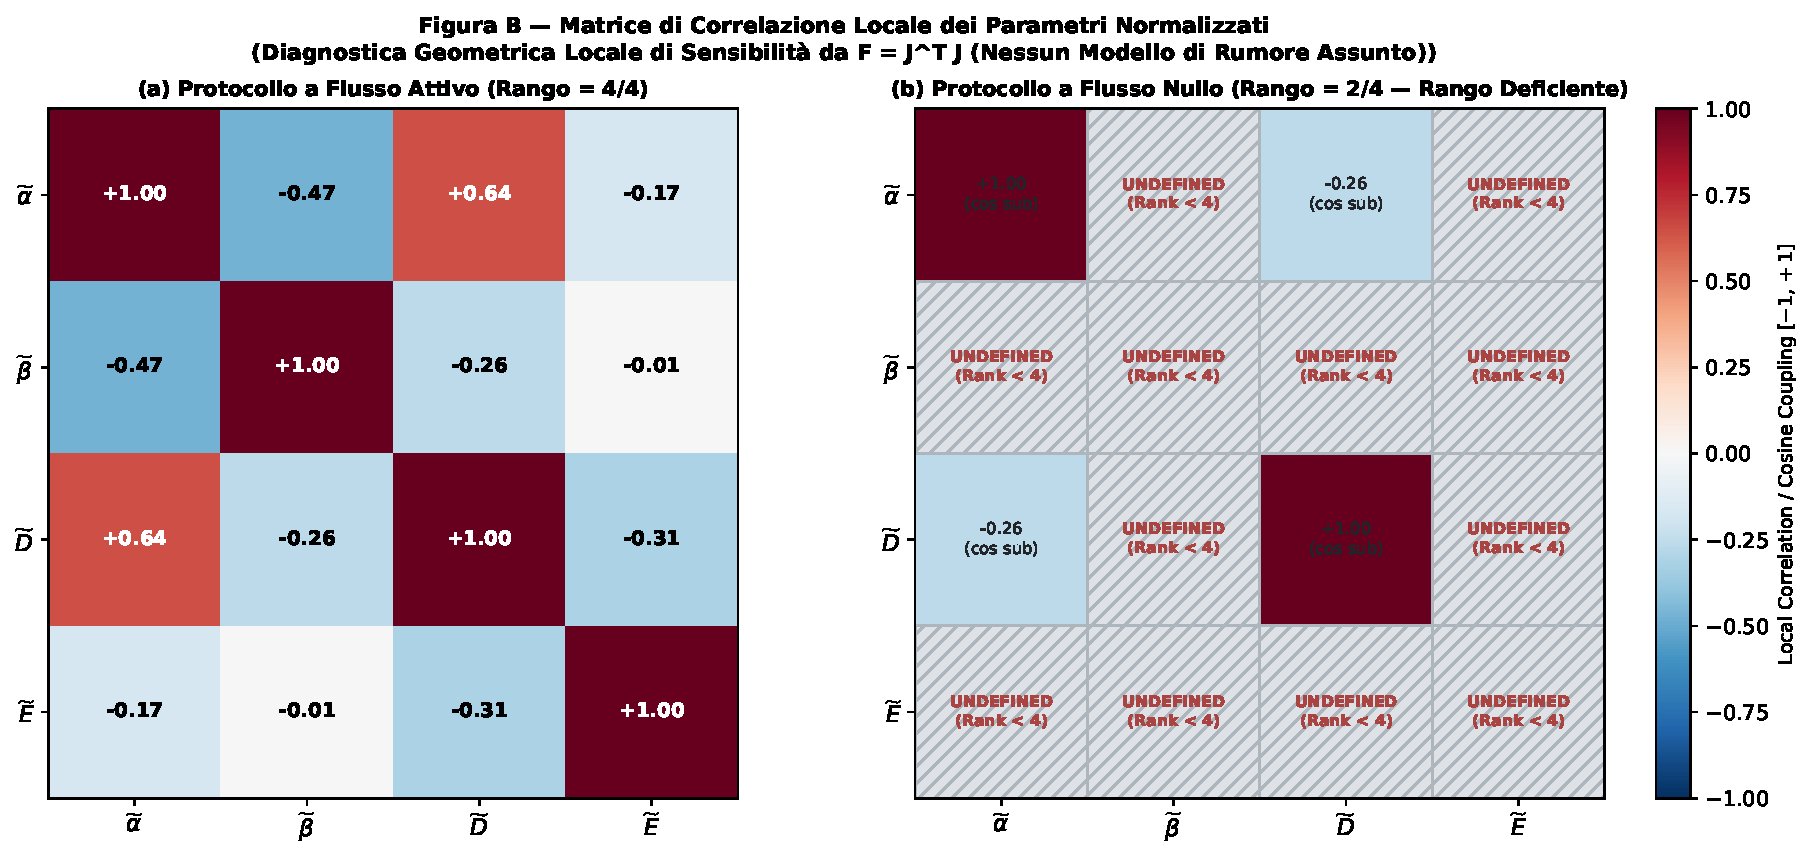
\includegraphics[width=0.85\linewidth]{appendices/figs_C01_local_correlation.pdf}
\caption{Il pannello (a) mostra la matrice di correlazione geometrica locale nel protocollo a flusso attivo; il pannello (b) mostra le similarità coseno tra le sole colonne non nulle nel protocollo a flusso nullo. Le celle tratteggiate indicano quantità non definite perché associate a colonne nulle del Jacobiano. La figura descrive la geometria locale della linearizzazione con pesi identità e non rappresenta correlazioni statistiche posteriori né ellissi di confidenza.}
\label{fig:app-local-geometry}
\end{figure}

\subsection{Transizione di sensibilità rispetto all'eccitazione}
\label{app:flow-transition}

La Tabella~\ref{tab:app-flow-sweep} riporta l'intera scansione del fattore $\kappa_q$. La soglia relativa del rango è $10^{-8}$; il numero di Péclet globale è definito dalla (\ref{eq:peclet-global}).

\begin{table}[H]
\centering
\caption{Scansione completa del Jacobiano sul quadrato unitario al variare del fattore comune di forzamento $\kappa_q$. Le ultime due colonne sono rispettivamente il valore singolare minimo e il numero di condizionamento completo.}
\label{tab:app-flow-sweep}
\small
\begin{tabular}{@{}rrrrrrr@{}}
\toprule
$\kappa_q$ & $\mathrm{Pe}_{\rm glob}$ & Rango & $\sigma_1$ & $\sigma_2$ & $\sigma_3$ & $\sigma_4$\\
\midrule
$0$ & $0$ & $2$ & $1.5833$ & $0.3222$ & $0$ & $0$\\
$10^{-3}$ & $0.003585$ & $4$ & $1.5827$ & $0.3223$ & $3.423\times10^{-4}$ & $5.957\times10^{-5}$\\
$10^{-2}$ & $0.03585$ & $4$ & $1.5775$ & $0.3224$ & $3.422\times10^{-3}$ & $5.954\times10^{-4}$\\
$0.05$ & $0.1793$ & $4$ & $1.5547$ & $0.3232$ & $1.7077\times10^{-2}$ & $2.970\times10^{-3}$\\
$0.10$ & $0.3585$ & $4$ & $1.5271$ & $0.3243$ & $3.4073\times10^{-2}$ & $5.917\times10^{-3}$\\
$0.25$ & $0.8964$ & $4$ & $1.4506$ & $0.3276$ & $8.451\times10^{-2}$ & $1.456\times10^{-2}$\\
$0.50$ & $1.7927$ & $4$ & $1.3457$ & $0.3331$ & $1.661\times10^{-1}$ & $2.801\times10^{-2}$\\
$1$ & $3.5854$ & $4$ & $1.2261$ & $0.3619$ & $2.924\times10^{-1}$ & $4.949\times10^{-2}$\\
$2$ & $7.1708$ & $4$ & $1.2924$ & $0.6129$ & $2.993\times10^{-1}$ & $6.045\times10^{-2}$\\
\bottomrule
\end{tabular}
\end{table}

\begin{table}[H]
\centering
\caption{Numero di condizionamento completo durante la scansione di eccitazione.}
\label{tab:app-flow-conditioning}
\small
\begin{tabular}{@{}rr@{}}
\toprule
$\mathrm{Pe}_{\rm glob}$ & $\kappa(J)$\\
\midrule
$0$ & indefinito ($\operatorname{rank}=2$)\\
$0.003585$ & $26571.23$\\
$0.03585$ & $2649.63$\\
$0.1793$ & $523.54$\\
$0.3585$ & $258.09$\\
$0.8964$ & $99.61$\\
$1.7927$ & $48.03$\\
$3.5854$ & $24.78$\\
$7.1708$ & $21.38$\\
\bottomrule
\end{tabular}
\end{table}

Il rango numerico pieno emerge già quando le colonne meccaniche sono piccole: la scala di $\sigma_4$ e il condizionamento sono quindi più informativi del solo rango.

\subsection{Identificabilità sulla mesh anatomica}
\label{app:anatomical-identifiability}

Sulla mesh BraTS da $3$ mm ($1901$ quadrilateri), con 180 osservazioni della concentrazione e valutazione $Q_1$ diretta, il caso a flusso nullo restituisce rango $2$ e spettro $(0.84817,0.08059,0,0)$. Con forzanti attive lo spettro è $(0.84027,0.05944,0.03197,0.001484)$, il rango è $4$ e $\kappa(J)=566.14$. La componente di $\widetilde\beta$ nel modo singolare meno informativo è $0.9983$. La griglia sensoriale è centrata sul centroide della lesione e ha semi-estensione di $25$ mm in entrambe le direzioni. Il protocollo costituisce una diagnostica locale su un caso anatomico sintetico.

\subsection{Sezioni unidimensionali e scansioni condizionali}

La distinzione interpretativa tra le diverse esplorazioni del paesaggio di costo è essenziale: una sezione unidimensionale (\emph{one-at-a-time}, Figura~\ref{fig:app-oat-slices}) valuta la variazione del funzionale mantenendo rigidi gli altri parametri al valore di riferimento, mentre una scansione condizionale (Figura~\ref{fig:app-beta-conditional}) esplora la dipendenza da $\beta$ fissando gli altri parametri alle stime ottenute da specifiche esecuzioni dell'ottimizzatore. Un profilo ottimizzato consente invece ai parametri di disturbo di compensare la variazione imposta su $\beta$. Per il protocollo considerato, il Jacobiano e i profili sono letti congiuntamente: la stabilità numerica delle derivate non elimina la debole informazione associata alla direzione meno sensibile.

\begin{figure}[htbp]
\centering
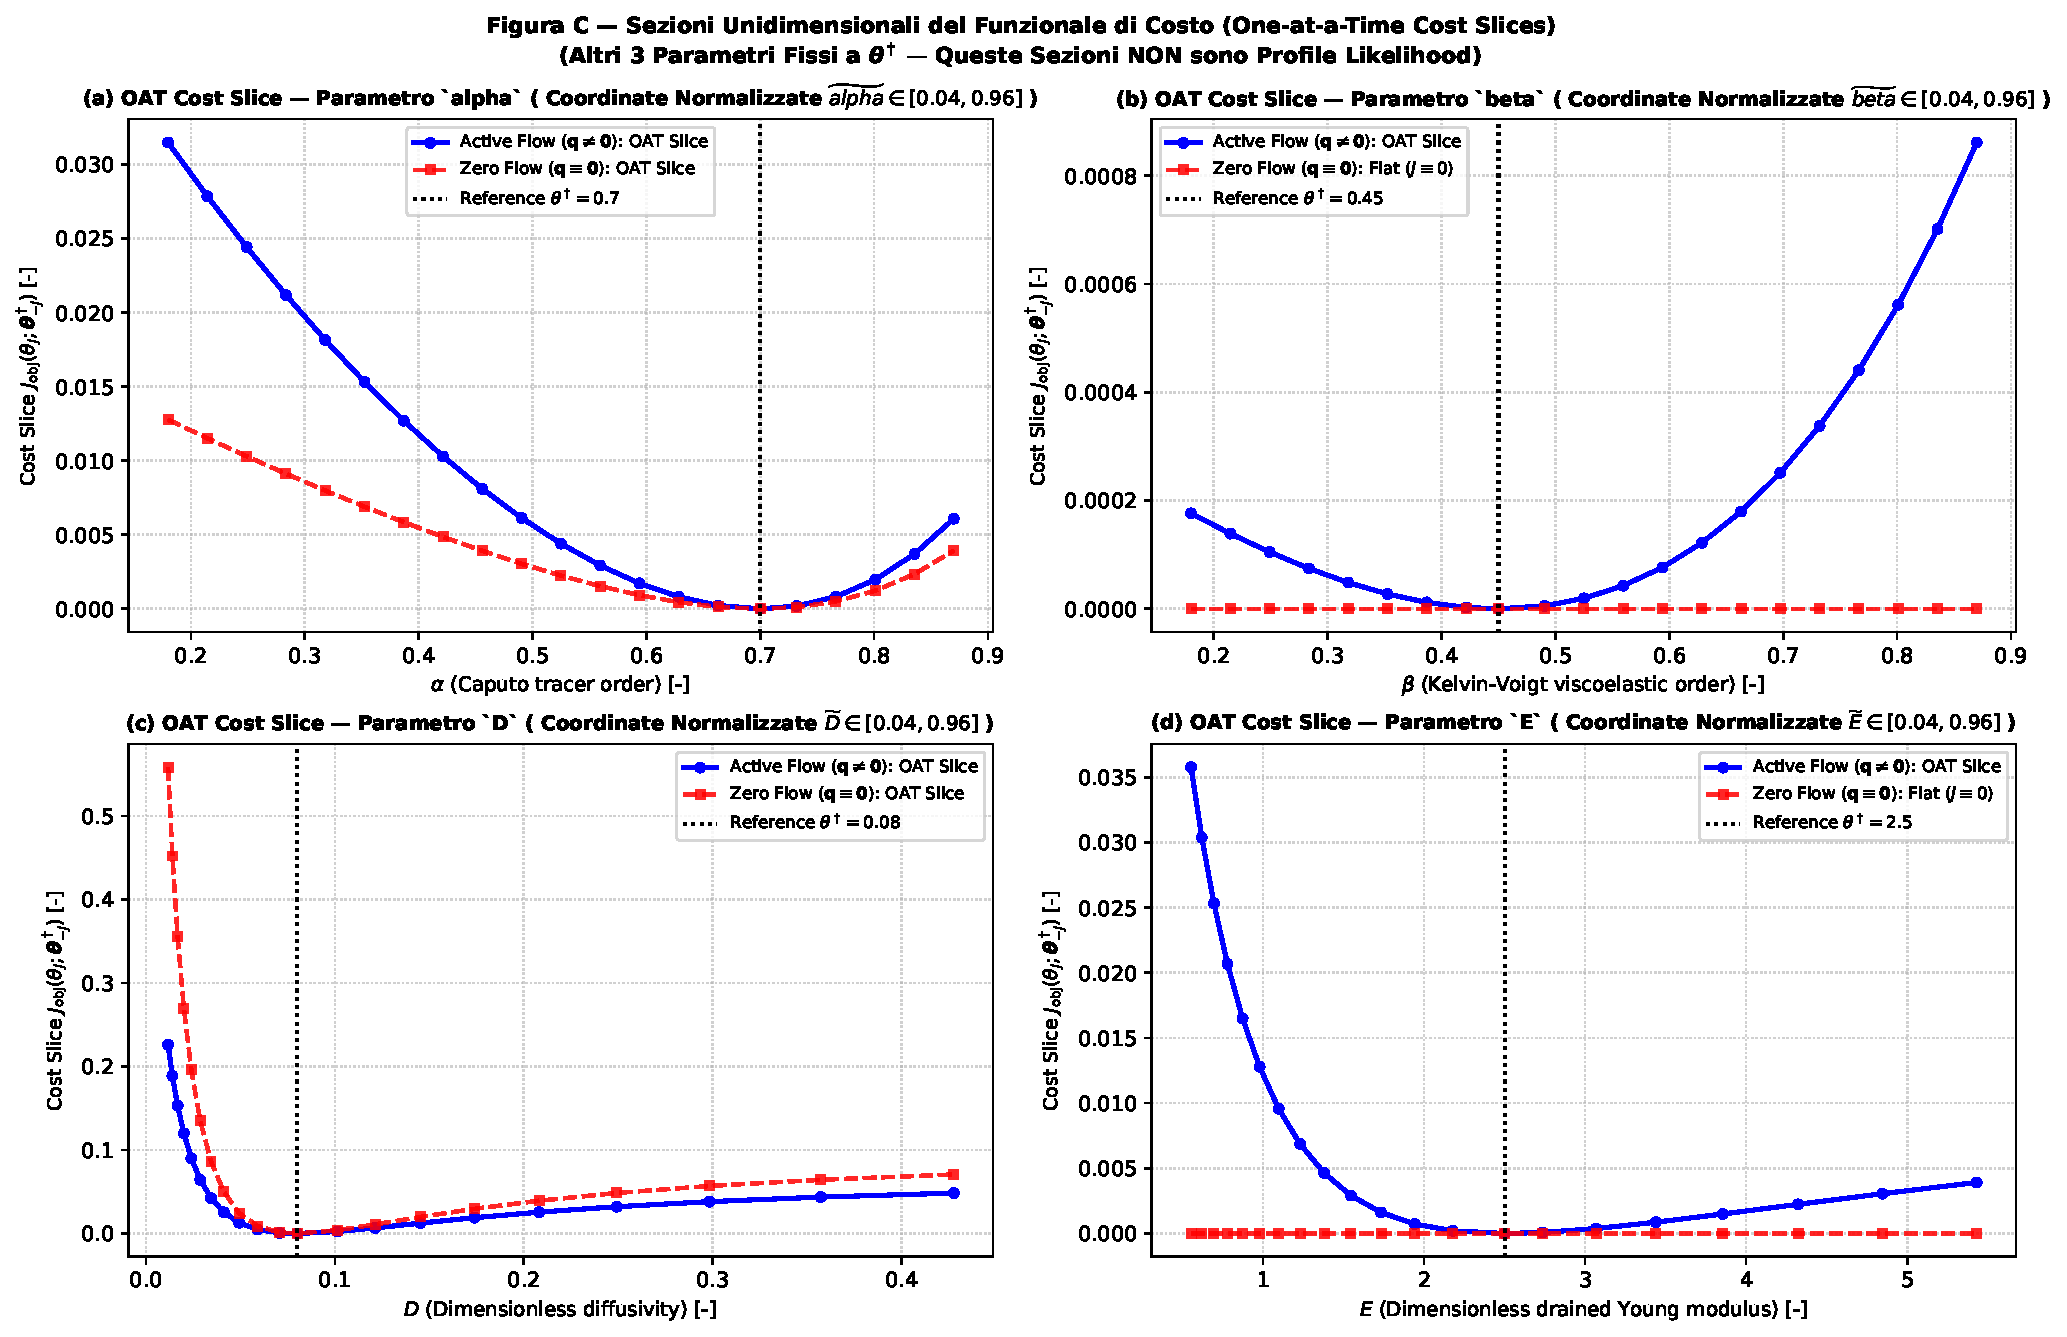
\includegraphics[width=0.8\textwidth]{appendices/figs_C02_one_at_a_time_cost_slices.pdf}
\caption{Sezioni unidimensionali (\emph{one-at-a-time}) del funzionale obiettivo: ciascun parametro varia singolarmente mentre i restanti sono mantenuti fissi al riferimento nominale. I profili piatti a flusso nullo per $\beta$ ed $E$ riflettono la degenerazione strutturale del modello; gli altri parametri sono mantenuti fissi.}
\label{fig:app-oat-slices}
\end{figure}

\begin{figure}[H]
\centering
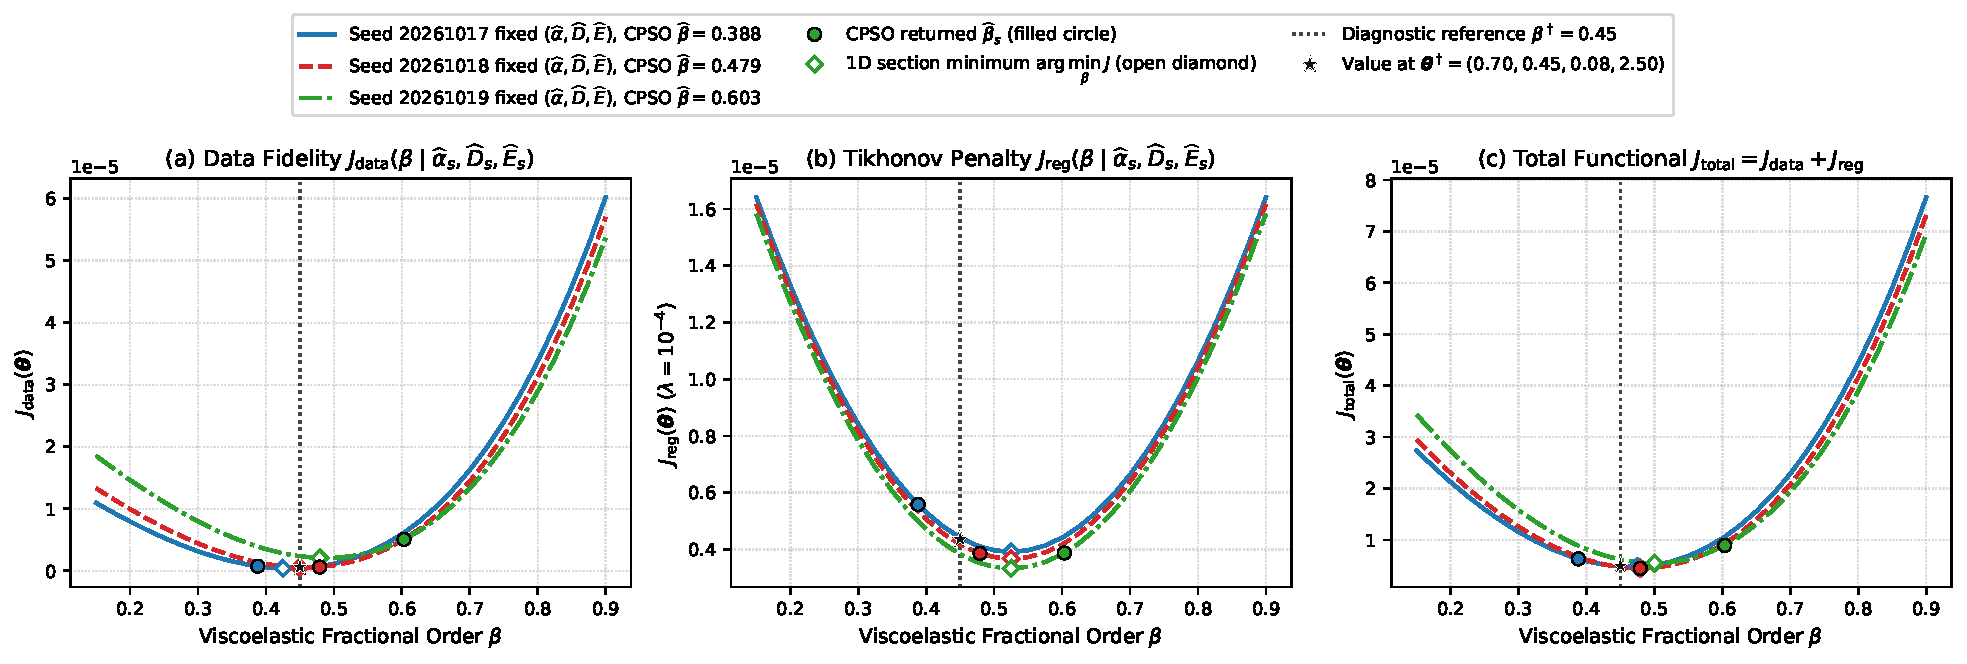
\includegraphics[width=0.8\linewidth]{appendices/figs_C03_beta_conditional_landscape.pdf}
\caption{Sezioni condizionali rispetto a $\beta$ ottenute fissando i parametri complementari ai valori finali delle tre esecuzioni CPSO senza rumore. La figura evidenzia la sensibilità del minimo apparente unidimensionale rispetto al contesto parametrico fissato e non sostituisce il profilo ottimizzato bidirezionale mostrato nella Figura~\ref{fig:beta-profiles}, nel quale i parametri di disturbo vengono ricalibrati ad ogni nodo.}
\label{fig:app-beta-conditional}
\end{figure}
\FloatBarrier
\section{Discretizzazione inversa e benchmark degli ottimizzatori}
\label{app:optimizer}
\setcounter{figure}{0}
\setcounter{table}{0}
\setcounter{equation}{0}

\subsection{Sensibilità del profilo di \texorpdfstring{$\beta$}{beta} alla griglia inversa}

Il target sintetico è stato mantenuto fisso a $(N,M)=(32,160)$, mentre la discretizzazione inversa è stata raffinata da $(16,80)$ a $(24,120)$. Il minimo campionato del profilo dati si sposta da $\beta=0.4500$ a $\beta=0.4375$. I parametri di disturbo $(\alpha,D,E)$ restano vicini tra le due risoluzioni; il termine dati al parametro vero diminuisce di un fattore $2.22$ e il minimo campionato del profilo di un fattore $3.53$ sulla griglia inversa più fine. Il confronto quantifica la sensibilità dei profili alla discretizzazione inversa. Le scansioni forward e backward sono procedure numeriche distinte; i valori riportati nel testo non vengono quindi interpretati come un’unica curva continua o come una prova di convergenza asintotica del problema inverso.


\subsection{Risultati per singola esecuzione}

Il benchmark comparativo impiega il medesimo target pulito congelato, la formulazione deterministica normalizzata (Modalità~A) con parametro di regolarizzazione $\lambda_A=10^{-4}$, centro a priori normalizzato $(0.5,0.5,0.5,0.5)$ e un budget massimo rigoroso di $600$ valutazioni effettive del solutore FEM per ciascuna esecuzione. Le tre esecuzioni CPSO provengono dalla campagna multi-seed precedente; hash del target, discretizzazioni e decomposizione del funzionale sono stati verificati rispetto ai relativi artefatti. Come dettagliato nella Tabella~\ref{tab:app-optimizer-runs}, una run di Differential Evolution si è arrestata a $588$ valutazioni per la tolleranza sulla dispersione della popolazione.

\begin{table}[H]
\centering
\caption{Risultati completi delle nove esecuzioni del benchmark a budget equivalente, con stime dei quattro parametri, costo totale finale e residuo osservativo relativo rispetto al target pulito. Il residuo è espresso in percentuale; la colonna delle valutazioni riporta il conteggio effettivo sul budget massimo pianificato.}
\label{tab:app-optimizer-runs}
\small
\setlength{\tabcolsep}{6.5pt}
\begin{tabular}{@{}lrrrrrrrr@{}}
\toprule
Metodo & Seed & Eval./600 & $\hat{\alpha}$ & $\hat{\beta}$ & $\hat{D}$ & $\hat{E}$ & $J_{\mathrm{total}}$ & $r_{\mathrm{clean}}$ [\%] \\
\midrule
CPSO                   & 20261017   & 600/600 & 0.7033 & 0.3880 & 0.07952 & 2.4788 & $6.3224\times10^{-6}$ & 0.2118 \\
CPSO                   & 20261018   & 600/600 & 0.6956 & 0.4791 & 0.07892 & 2.4805 & $4.4668\times10^{-6}$ & 0.1918 \\
CPSO                   & 20261019   & 600/600 & 0.6838 & 0.6033 & 0.07755 & 2.4870 & $8.9289\times10^{-6}$ & 0.5524 \\
\midrule
Differential Evolution & 2026120101 & 588/600 & 0.6964 & 0.4774 & 0.07901 & 2.4793 & $4.4626\times10^{-6}$ & 0.1851 \\
Differential Evolution & 2026120102 & 600/600 & 0.6964 & 0.4774 & 0.07901 & 2.4792 & $4.4626\times10^{-6}$ & 0.1851 \\
Differential Evolution & 2026120103 & 600/600 & 0.6964 & 0.4772 & 0.07901 & 2.4790 & $4.4627\times10^{-6}$ & 0.1848 \\
\midrule
Powell                 & 2026120201 & 600/600 & 0.6964 & 0.4774 & 0.07901 & 2.4794 & $4.4626\times10^{-6}$ & 0.1850 \\
Powell                 & 2026120202 & 600/600 & 0.6965 & 0.4773 & 0.07902 & 2.4791 & $4.4627\times10^{-6}$ & 0.1845 \\
Powell                 & 2026120203 & 600/600 & 0.6964 & 0.4774 & 0.07901 & 2.4793 & $4.4626\times10^{-6}$ & 0.1851 \\
\bottomrule
\end{tabular}
\end{table}

\subsection{Andamenti di convergenza e dispersione tra seed}

La storia di convergenza disponibile per la campagna multi-seed senza rumore è riportata nella Figura~\ref{fig:app-cpso-convergence-final}. Per i dieci twin experiments rumorosi sono disponibili riepiloghi finali e stime parametriche, ma non una cronologia completa verificabile del miglior candidato a ogni valutazione; non viene quindi rappresentata una traiettoria di convergenza per tali run. Il confronto diretto tra CPSO, Differential Evolution e il metodo di Powell basato su direzioni in termini di costo finale, residuo osservativo, recupero parametrico e traiettorie di discesa è illustrato nelle Figure~\ref{fig:app-optimizer-cost} e~\ref{fig:app-optimizer-convergence}.

La migliore esecuzione CPSO ($J_{\mathrm{total}}=4.4668\times10^{-6}$) raggiunge un costo vicino a quelli di Differential Evolution e Powell; la mediana CPSO è però più elevata e la dispersione tra inizializzazioni è maggiore, soprattutto per $\beta$. Il confronto descrive il comportamento dei metodi sul problema e sul budget considerati.

\begin{figure}[H]
\centering
\includegraphics[width=\linewidth]{03a_twin_noise_free_multistart/fig_multistart_convergence_v2.pdf}
\caption{Cronologia del miglior costo osservato nelle tre esecuzioni CPSO senza rumore. Tutte le run raggiungono il budget assegnato di 600 valutazioni; il grafico descrive la convergenza empirica di queste tre inizializzazioni e non certifica l’ottimalità globale.}
\label{fig:app-cpso-convergence-final}
\end{figure}

\begin{figure}[H]
\centering
\includegraphics[width=\linewidth]{12_optimizer_benchmark/fig_optimizer_benchmark_cost_and_errors.pdf}
\caption{Confronto descrittivo tra CPSO, Differential Evolution e Powell sul target sintetico congelato: costo finale e errori parametrici nel benchmark a tre repliche per metodo. Le differenze vanno interpretate nel quadro del budget e delle impostazioni riportati nel testo.}
\label{fig:app-optimizer-cost}
\end{figure}

\begin{figure}[H]
\centering
\includegraphics[width=\textwidth]{12_optimizer_benchmark/fig_optimizer_benchmark_convergence.pdf}
\caption{Traiettorie di convergenza delle nove esecuzioni del benchmark in funzione del numero di valutazioni effettive del solutore FEM. In questa campagna i valori finali raggiunti da Differential Evolution e Powell risultano più uniformi rispetto a CPSO; il risultato si riferisce al problema e alle impostazioni confrontate.}
\label{fig:app-optimizer-convergence}
\end{figure}
\FloatBarrier
\section{Rumore osservativo e risultati per realizzazione}
\label{app:noise}
\setcounter{figure}{0}\setcounter{table}{0}\setcounter{equation}{0}

\subsection{Twin cartesiani e controlli appaiati}
Il livello cartesiano nominale $\eta_{\infty}$ usa $\sigma=\eta_{\infty}\|\mathbf y^\dagger\|_\infty$; non va identificato con il livello anatomico $\eta_{\rm RMS}$ riferito al segnale bilanciato. Per ogni vettore di rumore la Tabella~\ref{tab:app-noisy-runs} riporta il rapporto realizzato $\eta_{\rm eff}=100\|\boldsymbol\epsilon\|_2/\|\mathbf y^\dagger\|_2$ e il residuo rispetto al target pulito. Il seed CPSO è $20261017$, la penalizzazione è $\lambda_B=7.2$ e tutte le esecuzioni raggiungono 600 valutazioni FEM. La mediana degli errori si ottiene calcolando prima, su ciascuna riga, $100|\widehat u-u^\dagger|/|u^\dagger|$.

\begin{table}[H]
\centering
\caption{Dieci inversioni cartesiane con seed dell'ottimizzatore fissato. $\eta_{\rm eff}$ e $r_{\rm clean}$ sono percentuali.}
\label{tab:app-noisy-runs}
\small
\setlength{\tabcolsep}{7pt}
\begin{tabular}{@{}cccrrrrr@{}}
\toprule
$\eta_{\mathrm{nom}}$ & Seed dati & $\eta_{\mathrm{eff}}$ [\%] & $\hat{\alpha}$ & $\hat{\beta}$ & $\hat{D}$ & $\hat{E}$ & $r_{\mathrm{clean}}$ [\%] \\
\midrule
$0.05$ & 2026110501 & $9.47$  & $0.6447$ & $0.3562$ & $0.07603$ & $2.5247$ & $1.326$ \\
$0.05$ & 2026110502 & $8.60$  & $0.6799$ & $0.4020$ & $0.07797$ & $2.2431$ & $0.886$ \\
$0.05$ & 2026110503 & $8.85$  & $0.7027$ & $0.5192$ & $0.08064$ & $2.9619$ & $1.075$ \\
$0.05$ & 2026110504 & $8.41$  & $0.7301$ & $0.4119$ & $0.08758$ & $2.6127$ & $1.156$ \\
$0.05$ & 2026110505 & $9.49$  & $0.7275$ & $0.3782$ & $0.08377$ & $3.1846$ & $1.587$ \\
\midrule
$0.10$ & 2026111001 & $17.95$ & $0.6272$ & $0.4754$ & $0.06897$ & $1.6559$ & $3.607$ \\
$0.10$ & 2026111002 & $15.96$ & $0.7151$ & $0.4555$ & $0.07524$ & $2.2282$ & $1.320$ \\
$0.10$ & 2026111003 & $16.92$ & $0.6686$ & $0.4234$ & $0.07587$ & $2.4618$ & $0.737$ \\
$0.10$ & 2026111004 & $16.94$ & $0.7478$ & $0.3476$ & $0.08816$ & $2.7267$ & $1.347$ \\
$0.10$ & 2026111005 & $17.00$ & $0.6847$ & $0.3811$ & $0.07748$ & $2.1509$ & $1.118$ \\
\bottomrule
\end{tabular}
\end{table}

\paragraph{Controlli a dati identici.}\label{app:noise-controls}
Per i cinque vettori al $10\%$ si ripete l'inversione con $\lambda_B=1.8$ e seed CPSO $20261017$ e $20261018$. Sul dato $2026111003$ si ottengono $(\widehat\beta,\Jfun)=(0.4058,85.4902)$ e $(0.8598,84.3620)$. La variazione del seed riguarda soltanto l'inizializzazione dello sciame. Powell riutilizza i cinque campioni di ciascun livello con $(\eta,\lambda_B)=(0.05,7.2)$ e $(0.10,1.8)$. Le mediane per metodo e i relativi estremi sono nella Tabella~\ref{tab:noisy-controls-beta}.

\subsection{Repliche anatomiche nel modello tangentale}
Per il disegno $d$ si costruiscono dati $\mathbf y_d^\dagger+\sigma_\eta\xi^{(r)}$, con $\xi^{(r)}\sim\mathcal N(0,I_{80})$ e $\sigma_\eta=\eta\,\mathrm{RMS}(\mathbf y^\dagger_{\rm bil})$. Il problema a sei incognite usa il Jacobiano grezzo congelato e il vincolo $\mathbf0\leq\mathbf z\leq\mathbf1$. A ogni livello si riutilizzano i 50 vettori standard generati con seed $20261111$. La tabella seguente esprime i risultati come conteggi espliciti. Per entrambi i disegni la Tabella~\ref{tab:pv-noise-linear} contiene anche i MAE e le deviazioni standard locali non vincolate.

\begin{table}[H]\centering\small
\caption{Repliche tangentali a sei parametri. Una stima è classificata al bordo se $z_\beta$ dista meno di $10^{-5}$ da uno dei due estremi.}
\label{tab:app-tangent-counts}
\begin{tabular}{@{}lrrrr@{}}\toprule
Sensori & $0.1\%$ RMS & $0.5\%$ RMS & $1\%$ RMS & $5\%$ RMS\\\midrule
Bilanciati & 0/50 & 0/50 & 8/50 & 37/50\\
Nell'edema & 0/50 & 17/50 & 26/50 & 39/50\\\bottomrule
\end{tabular}
\end{table}

\subsection{Pilota non lineare a quattro parametri}
Ogni replica del pilota usa i sensori bilanciati e richiede nuove valutazioni FEM. La Tabella~\ref{tab:app-fem-cases} identifica i denominatori dei risultati \emph{già consolidati al momento della stesura}: otto repliche della campagna estesa allo $0.1\%$ e due casi della campagna separata di validazione ad alto rumore al $5\%$. Le due righe al $5\%$ non sono state conteggiate come parte delle otto repliche previste nella campagna estesa. A ogni livello, due partenze sullo stesso dato contribuiscono a una sola stima. I costi sono $J_{\rm data}=\|\mathbf r\|_2^2/(2\sigma_\eta^2)$.

\begin{table}[H]\centering\small
\caption{Esiti documentati del pilota FEM. La prima riga aggrega otto repliche. Le successive riportano separatamente le due repliche convergenti al livello più alto.}
\label{tab:app-fem-cases}
\begin{tabular}{@{}lrlrr@{}}\toprule
Livello & $n$ & Stime di $\beta$ & $J_{\rm data}(\theta^\dagger)$ & $J_{\rm data}(\widehat\theta)$\\\midrule
$0.1\%$ & 8 & media $0.4427$, estremi $[0.3878,0.5018]$ & --- & ---\\
$5\%$ & 1 & $0.9000$ & 31.24 & 30.30\\
$5\%$ & 1 & $0.1500$ & 38.06 & 37.37\\\bottomrule
\end{tabular}
\end{table}

Gli errori assoluti delle due repliche al $5\%$ sono $0.4500$ e $0.3000$. La loro media è $0.3750$, a fronte di $0.0259$ nelle otto repliche allo $0.1\%$. Il denominatore disponibile al $5\%$ in questa versione è quello dei due casi convergenti documentati \emph{nella validazione separata}: non autorizza a dedurre una probabilità di saturazione. Per $0.5\%$ e $1\%$, i risultati definitivi qui riportati appartengono esclusivamente alla campagna tangentale a sei parametri. I nuovi risultati della campagna FEM estesa vanno inseriti qui e nella Tabella~\ref{tab:pv-noise-fem} solo dopo il controllo di completezza, degli arresti e delle stime ai vincoli.

\FloatBarrier
\section{Diagnostica della pesatura e della regolarizzazione}
\label{app:objective}

Sono stati confrontati tre modi di pesatura. Per la campagna sintetica, $s_{\rm ref}=\|\mathbf y_{\rm clean}\|_\infty$ e, per $\eta>0$, $\sigma=\eta s_{\rm ref}$. Le matrici di peso sono $W_A=I/(\sqrt{N_{\rm obs}}s_{\rm ref})$, $W_{B,\rm mean}=I/(\sqrt{N_{\rm obs}}\sigma)$ e $W_{B,\rm cov}=I/\sigma$. Di conseguenza, a parità di residuo, $J_{\rm data}^{B,\rm mean}/J_{\rm data}^{A}=\eta^{-2}$ e $J_{\rm data}^{B,\rm cov}/J_{\rm data}^{A}=N_{\rm obs}/\eta^2$. Nel modo covariance, $W^\mathsf TW=\Sigma^{-1}$ per $\Sigma=\sigma^2I$. Quando $\eta=0$, la covarianza non è invertibile e si usa soltanto la normalizzazione deterministica.

\begin{table}[H]
\centering
\caption{Confronto del termine dati per $\theta^\dagger$ al livello nominale di rumore 10\%, con $\lambda=10^{-4}$.}
\label{tab:weights}
\small
\begin{tabular}{lrr}
\toprule
Modo & $J_{\rm data}$ & $J_{\rm reg}$\\
\midrule
Deterministico $L^\infty$ & $4.119\cdot10^{-3}$ & $4.363\cdot10^{-6}$\\
Noise-weighted mean & $4.119\cdot10^{-1}$ & $4.363\cdot10^{-6}$\\
Noise-weighted covariance & $7.4144\cdot10^{1}$ & $4.363\cdot10^{-6}$\\
\bottomrule
\end{tabular}
\end{table}

La griglia di sensibilità a $\lambda$ comprende otto valori ($0$, $10^{-7}$, $10^{-6}$, $10^{-5}$, $10^{-4}$, $10^{-3}$, $10^{-2}$, $10^{-1}$), due convenzioni di pesatura (deterministica e noise-weighted mean), tre livelli di rumore ($\eta=0$, $0.01$, $0.05$) e sette candidati fissati. Le 336 righe sono valutazioni del funzionale su candidati preesistenti, non 336 ottimizzazioni. La convenzione noise-weighted covariance è analizzata nella tabella precedente, ma non è inclusa nella griglia di sensibilità a $\lambda$. L'esperimento non calibra automaticamente $\lambda$ e non deve usare la conoscenza di $\theta^\dagger$ per selezionare il parametro di regolarizzazione.

\begin{figure}[H]
\centering
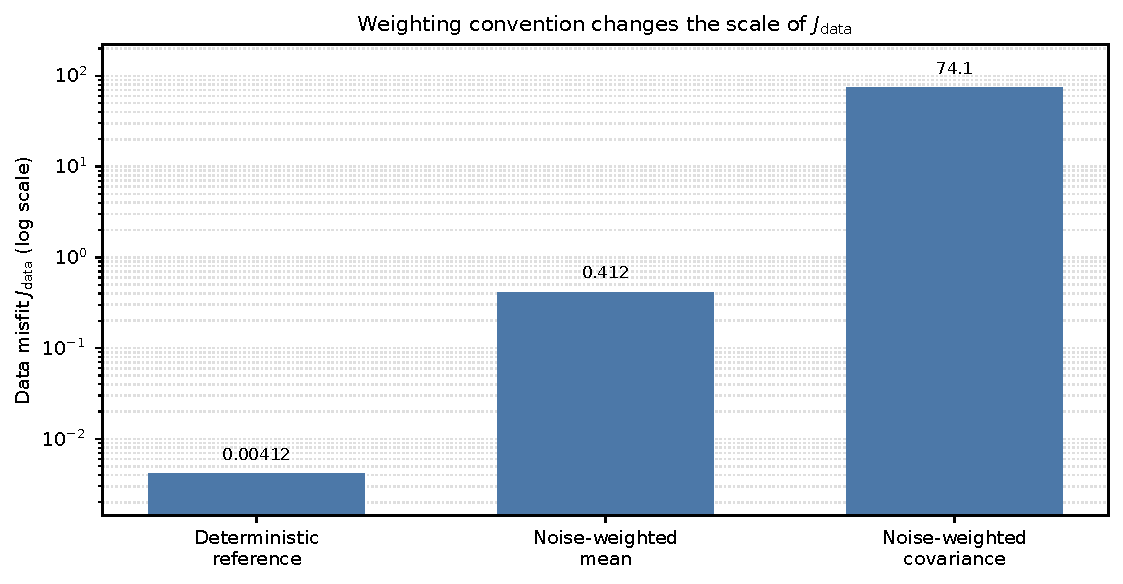
\includegraphics[width=0.47\textwidth]{appendices/figs_016_objective_weight_modes.pdf}
\caption{Effetto della convenzione di pesatura sul termine dati $J_{\rm data}$ per il parametro vero sintetico $\theta^\dagger$, rumore nominale $\eta=10\%$ e $\lambda=10^{-4}$. I valori sono $4.119\times10^{-3}$ (riferimento deterministico), $0.4119$ (noise-weighted mean) e $74.144$ (covarianza inversa esatta). Il termine di regolarizzazione resta $4.363\times10^{-6}$; le scale del costo dati, e quindi il compromesso con la penalizzazione, dipendono dalla convenzione.}
\end{figure}
\begin{figure*}[t]
\centering
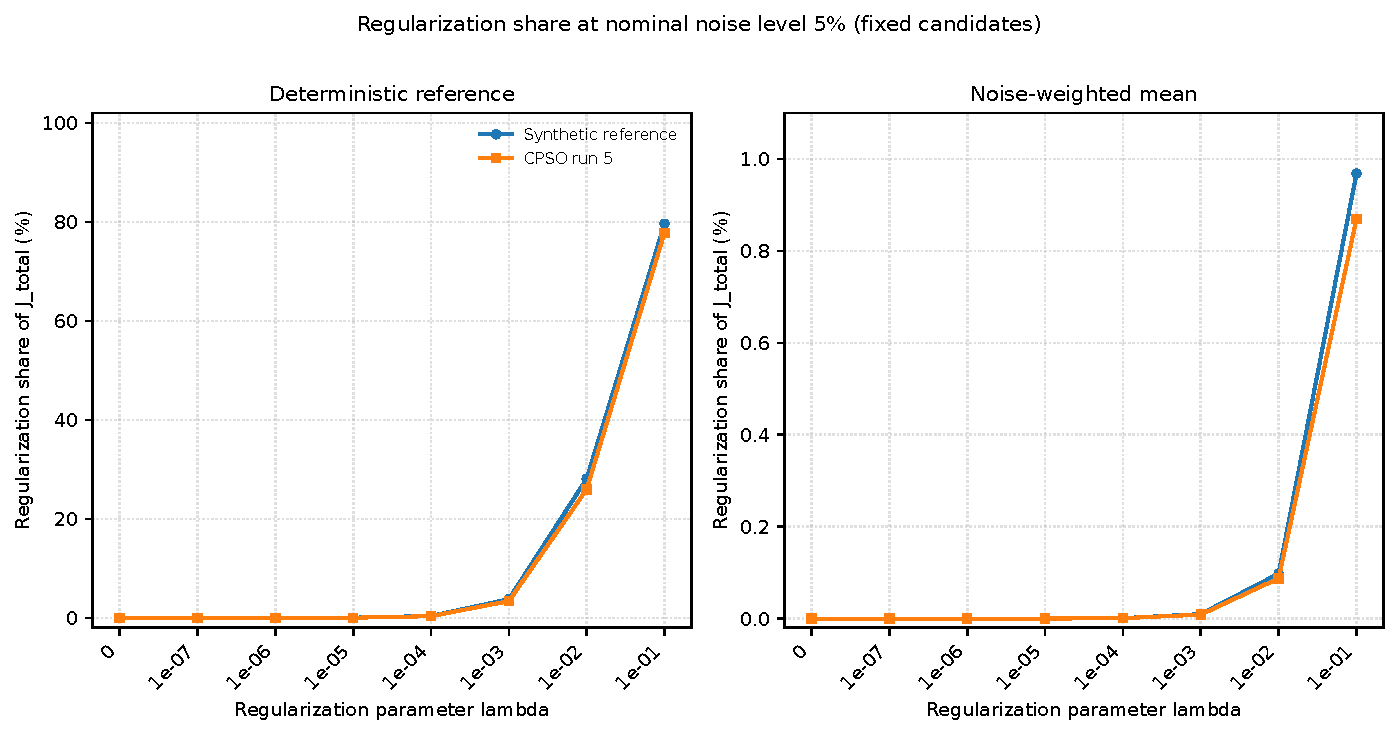
\includegraphics[width=0.94\textwidth]{appendices/figs_017_lambda_grid.pdf}
\caption{Quota del termine di regolarizzazione nel costo totale in funzione di $\lambda$, al livello nominale di rumore del 5\%, per due candidati fissati. I pannelli usano scale verticali distinte per rendere leggibili entrambe le convenzioni: i valori non vanno confrontati come se condividessero la stessa scala. La figura è una valutazione diagnostica del funzionale, non una curva di ottimizzazione.}
\end{figure*}

\subsection{Verifica della conversione di scala usata nella campagna finale}

Nella campagna finale rumorosa si impiega Mode B covariance, cioè $W^{\mathsf T}W=\Sigma^{-1}=\sigma^{-2}I$, con $N_{\rm obs}=180$ e scala di riferimento $\eta_{\rm ref}=0.05$. Il valore di conversione equivalente a un dato livello $\eta$ è
\[
\lambda_B^{\rm eq}(\eta)=\frac{N_{\rm obs}}{\eta^2}\lambda_A.
\]
Pertanto, con $\lambda_A=10^{-4}$, si ottiene $\lambda_B^{\rm eq}(0.05)=7.2$, mentre $\lambda_B^{\rm eq}(0.10)=1.8$. Nel protocollo congelato è stato mantenuto $\lambda_B=7.2$ per entrambe le classi rumorose. Questa scelta conserva l'equivalenza di scala soltanto a $\eta=0.05$; a $\eta=0.10$ la regolarizzazione ha peso relativo quattro volte maggiore rispetto a quello del protocollo equivalente. Non è quindi corretto attribuire le differenze osservate tra i due gruppi esclusivamente all'aumento del rumore. Il contratto numerico è stato testato prima di eseguire le run rumorose.

\begin{table}[H]
\centering
\caption{Audit numerico della conversione di scala nella campagna finale, valutato sul medesimo residuo di prova.}
\label{tab:normalization-contract}
\small
\begin{tabular}{lr}
\toprule
Controllo & Valore osservato\\
\midrule
Fattore atteso $N_{\rm obs}/\eta_{\rm ref}^2$ & $72000$\\
Rapporto $J_{\rm data}^{B}/J_{\rm data}^{A}$ & $72000$\\
Rapporto $J_{\rm reg}^{B}/J_{\rm reg}^{A}$ & $72000$\\
Rapporto $J_{\rm total}^{B}/J_{\rm total}^{A}$ & $72000$\\
Isolamento del target pulito & verificato\\
Decomposizione $J_{\rm total}=J_{\rm data}+J_{\rm reg}$ & verificata\\
\bottomrule
\end{tabular}
\end{table}

La conversione rende equivalente il rapporto fra termine dati e regolarizzazione al livello di riferimento $\eta_{\rm ref}=0.05$ per il residuo usato nel controllo. La stessa costante $\lambda_B$ è stata poi mantenuta per entrambe le classi rumorose; poiché $\sigma$ dipende dal livello $\eta$, il bilanciamento relativo non è esattamente invariato tra $\eta=0.05$ e $\eta=0.10$. Questa scelta è da documentare e non deve essere descritta come una calibrazione automatica ottimale della regolarizzazione.

\FloatBarrier
\section{Riproducibilità computazionale e provenienza}
\label{app:repro}

\subsection{Provenienza della campagna finale di twin experiments}

Il target sintetico finale è stato riutilizzato senza rigenerazione e verificato tramite SHA-256 \texttt{1bca9e29\allowbreak{}c60d77c1\allowbreak{}450fd2fc\allowbreak{}ea845d23\allowbreak{}20c9e449\allowbreak{}45dd7d3c\allowbreak{}cda52aa3\allowbreak{}3ef261af}. La discretizzazione target è $(N,M)=(32,160)$, quella inversa principale $(N,M)=(16,80)$ e il numero di osservazioni è 180. La baseline senza rumore riutilizza tre run con seed CPSO 20261017, 20261018 e 20261019. La campagna rumorosa usa il seed CPSO 20261017 e i seed dati $(2026110501,\ldots,2026110505)$ per $\eta=0.05$ e $(2026111001,\ldots,2026111005)$ per $\eta=0.10$. Il protocollo pianifica 600 valutazioni FEM per run; gli artefatti JSON registrano la storia completa, il costo migliore, la condizione di arresto e i controlli di integrità.

Il test di integrità della campagna finale non sostituisce una validazione indipendente del modello fisico né una verifica di convergenza dell'ottimizzatore. Prima della sottomissione, l'archivio pubblico versionato dovrà contenere i sorgenti effettivamente usati, le configurazioni, le dipendenze, gli artefatti JSON/CSV e i log necessari per riprodurre i numeri inclusi nel manoscritto.

\subsection{Ambiente software e suite di test}

Il report di provenienza archiviato per il commit \texttt{2c10b387833dd81fbae3654597bdcad823cacfeb} registra 37 test superati in 57.66 s nell'ambiente dichiarato: macOS 26.5.1 su arm64, Python 3.11.17 e deal.II indicato nel file di ambiente. Questo conteggio va associato alla specifica snapshot documentata dal report; prima della sottomissione, la suite deve essere rieseguita sul commit esatto destinato al rilascio. Il file \texttt{environment\_provenance.json}, il lock Conda, i report JSON, le matrici Jacobiane, le tabelle CSV, le mesh e i log originali sono inclusi nell'archivio sorgente consegnato con il manoscritto.

I test elencati nel report comprendono formule e limiti dell'operatore L1, compatibilità iniziale, identità energetica e massa discreta, MMS accoppiato, non-identificabilità a flusso nullo, controlli della pipeline anatomica, integrazione di mesh quadrilatere, retrocompatibilità MMS, norma vettoriale $L^2$ ed entry point CLI. Il passaggio dei test supporta la riproducibilità del comportamento verificato nei casi coperti, ma non dimostra da solo correttezza fisica generale o validità clinica.

\subsection{Provenienza del caso anatomico}

I report della geometria contengono SHA-256 e percorsi degli input MRI effettivamente usati. L'identità dei file e la griglia NIfTI vengono quindi tracciate nel bundle; la provenienza ufficiale del dataset deve essere attestata tramite la fonte BraTS e le condizioni di accesso, non dal solo hash. Il soggetto è un singolo caso del benchmark. Le forzanti, i campi temporali e i dati per i twin experiments sono sintetici.

\FloatBarrier

\end{document}